\documentclass[]{thesis}
\usepackage{thesis}
\usepackage{parskip}
\usepackage{hepnames}
\usepackage[printonlyused]{acronym}
\usepackage{ptdr-definitions}
\usepackage{LC-shortcuts}
\usepackage{slashed}
\usepackage{multirow}
\usepackage{multicol}
\usepackage{amssymb}
\usepackage{import}
\usepackage{colortbl}
\usepackage{hhline}
\usepackage{feynmp}


%% You can set the line spacing this way
%\setallspacing{double}
%% or a section at a time like this
%\setfrontmatterspacing{double}


%% Define a few useful shorthands
\newcommand{\emu}{\Pe\Pgm}
\newcommand{\ee}{\Pe\Pe}
\newcommand{\mumu}{\Pgm\Pgm}
\newcommand{\mutau}{\Pgm\Pgth}
\newcommand{\etau}{\Pe\Pgth}
\newcommand{\tautau}{\Pgth\Pgth}

\newcommand{\WJets}{\ensuremath{\PW}{+}\text{jets}\xspace}
\newcommand{\mhmax}{\ensuremath{m_{\Ph}^{\text{max}}}\xspace}
\newcommand{\ttbar}{\ensuremath{\Pqt\Paqt}\xspace}
\newcommand{\ZToTauTau}{\ensuremath{\PZ\to\Pgt\Pgt}\xspace}
\newcommand{\HToTauTau}{\ensuremath{\PH\to\Pgt\Pgt}\xspace}

\renewcommand{\listfigurename}{List of figures}
\renewcommand{\listtablename}{List of tables}


\DeclareGraphicsRule{.1}{mps}{*}{}
\DeclareGraphicsRule{.2}{mps}{*}{}
\DeclareGraphicsRule{.3}{mps}{*}{}
\DeclareGraphicsRule{.4}{mps}{*}{}
\DeclareGraphicsRule{.5}{mps}{*}{}
\DeclareGraphicsRule{.6}{mps}{*}{}
\DeclareGraphicsRule{.7}{mps}{*}{}
\DeclareGraphicsRule{.8}{mps}{*}{}
\DeclareGraphicsRule{.9}{mps}{*}{}
\DeclareGraphicsRule{.10}{mps}{*}{}
\DeclareGraphicsRule{.11}{mps}{*}{}
\DeclareGraphicsRule{.12}{mps}{*}{}
\DeclareGraphicsRule{.13}{mps}{*}{}
\DeclareGraphicsRule{.14}{mps}{*}{}


%% PDF metadata
\makeatletter
\@ifpackageloaded{hyperref}{%
\hypersetup{%
hidelinks=true,
pdftitle = {Observation of the Higgs boson decaying to photons with the CMS detector},
pdfsubject = {Louie Dartmoor Corpe's PhD thesis},
pdfkeywords = {CMS, H, physics, LHC, Higgs},
pdfauthor = {\textcopyright\ Louie Dartmoor Corpe},
linkcolor=black,
colorlinks=false
}
}{}
\makeatother

%% Define the thesis title and author
\title{Observation of the Higgs boson decaying to photons with the CMS detector using p-p collisions at 13 TeV}
\author{Louie Dartmoor Corpe}

%% Start the document
\begin{document}

\begin{fmffile}{thesisfeynmandiags}
%% Define the un-numbered front matter (cover pages, rubrik and table of contents)
\begin{frontmatter}
  %% Title
%??UPDATE THIS
\titlepage[Imperial College London\\Department of Physics]%
{A dissertation submitted to Imperial College London\\
  for the degree of Doctor of Philosophy}
\newpage
The copyright of this thesis rests with the author and is made available under a Creative Commons
Attribution Non-Commercial No Derivatives licence. Researchers are free to copy, distribute or
transmit the thesis on the condition that they attribute it, that they do not use it for commercial
purposes and that they do not alter, transform or build upon it. For any reuse or redistribution,
researchers must make clear to others the licence terms of this work.

%% Abstract
\begin{abstract}%[\smaller \thetitle\\ \vspace*{1cm} \smaller {\theauthor}]
  %\thispagestyle{empty}
A study of \Hgg with \thisanalysislumi\ifb of data from \pp collisions at $\sqrt{s}=13\TeV$ is presented. The data were collected at the start of LHC \RunII by the CMS experiment between April and \finaldatatakingmonth 2016. The result is an new standalone observation of the Higgs boson in the diphoton decay channel.  
The significance of the excess is observed to be $\obsSigAtRunIBF\sigma$ ($\expSigAtRunIBF\sigma$ expected) at the combined \RunI best-fit $\mH=125.09\GeV$. The maximum significance of $\obsSigAtMin\sigma$ ($\expSigAtMin\sigma$ expected) is observed at $\mH=\bestFitGlobalMH\GeV$.
The measured Higgs boson signal strength is $\obsMuBreakdown$. 
The signal strength is measured separately for: fermionic and bosonic production modes, giving $ \obsMuV$ and $\obsMuF$; 
\ifNewAnalysis
and for the ggH, VBF, ttH and VH production modes, giving $\obsMuggH$, $\obsMuVBF$, $\obsMuttH$, and $\obsMuVH$, .
\else
and for the ggH, VBF and ttH production modes, giving $\obsMuggH$, $\obsMuVBF$, and $\obsMuttH$.
\fi
Measurements of the Higgs boson coupling modifiers yield $\obskF$, $\obskV$ for the fermionic and bosonic coupling modifiers and $\obskGlu$, $\obskGlu$ for the effective coupling modifiers.
All measurements are found to be consistent with the theoretical expectation for a SM-like Higgs boson.
\end{abstract}

%% Declaration
\begin{declaration}
The results presented in this thesis are the culmination of work which I certify to be my own, although it is based in part on studies by others. The theory described in \Chap~\ref{chap:theory} has been summarised in my words, but was produced by theorists. The LHC and CMS design and performance detailed in \Chap~\ref{chap:detector} are the result of studies by other experimentalists, although I was involved in the \RunI photon energy resolution measurements (see \Sec~\ref{sec:cms:ecal:overview}) and \RunII ECAL calibration (see \Sec~\ref{sec:cms:ecal:calibration}).
\Chap\s~\ref{chap:reconstruction} and~\ref{chap:categorisation} are the work of various individuals in the CMS collaboration and \Hgg group, of which I am a member. Some of the procedures are therefore the work of my collaborators.

The bulk of my personal work is presented in \Chap\s~\ref{chap:model} and~\ref{chap:statandresults}, which detail the signal and background modelling, handling of systematic uncertainties, statistical interpretation of the data and production of results. Indeed, these were my personal areas of responsibility in the CMS \Hgg group. 
\ifNewAnalysis
I was responsible for these topics for two studies of \Hgg with \RunII data~\cite{CMS-PAS-HIG-15-005,CMS-PAS-HIG-16-020}. The analysis presented here considers substantially more data. It also includes significant developments to the parametric signal modelling techniques with were conceived and implemented by me, and which I used to produce the results, but which do not feature in previous results.  
\else
I was responsible for these topics for two studies of \Hgg with \RunII data~\cite{CMS-PAS-HIG-15-005,CMS-PAS-HIG-16-020}, the latter being the basis for this thesis. These chapters also include significant developments to the parametric signal modelling techniques with were conceived and implemented by me, and which I used to produce the results, but which do not feature in~\cite{CMS-PAS-HIG-16-020}.  
\fi

Where ideas or figures from others are used, appropriate sources are referenced. Figures labelled ``\textbf{CMS}'' are either taken from CMS publications or preliminary public documents, including those produced by me, and are referenced appropriately; or result from the analysis I have performed in this thesis, in which case they have been approved by the CMS collaboration. Figures additionally labelled ``\Hgg'' result from the work of members of the CMS Higgs to diphoton analysis group specifically.
  %\vspace*{0.5cm}
  \begin{flushright}
    Louie Dartmoor Corpe
  \end{flushright}
\end{declaration}


%% Acknowledgements
\begin{acknowledgements}
To be written!\\
- family\\
- supervisors\\
- friends\\
- IC HEP, CMS, Hgg group\\
- STFC\\
- Emma \\
\end{acknowledgements}


%% Preface
%\begin{preface}
%\end{preface}

%% ToC
\tableofcontents

\renewcommand{\listfigurename}{List of figures}
\renewcommand{\listtablename}{List of tables}

\listoffigures
\listoftables

%% Strictly optional!
\frontquote%
{There are more things in heaven and earth, Horatio, \\
Than are dreamt of in your philosophy} 
  {Hamlet (William Shakespeare)}

\end{frontmatter}

%% Start the content body of the thesis
\begin{mainmatter}
  %% Actually, more semantic chapter filenames are better, like "chap-bgtheory.tex"
  \cleardoublepage
  \pagenumbering{arabic}
  \chapter{Introduction and theory}
\label{chap:theory}

\section{The Standard Model of particle physics}
\subsection{Introduction}

The \SM of particle physics was formulated in the second half of the 20$^{\text{th}}$ century. It has been an immensely successful theory, accurately describing all known processes in high energy physics encountered thus far. The \SM is a gauge theory, in particular a \QFT, in which the universe is made up of interacting fields. In this model, the fundamental elements of matter can be represented as relativistic quantum fields, the excitations of which are manifested as particles. Furthermore, the fundamental forces which govern the interactions of matter can be described the exchange of mediator particles. The \SM places the electromagnetic, strong and weak forces into one framework. The only force which is not described not the \SM is gravity, since no viable quantum theory of gravity currently exists. This does not affect the predictive power of the \SM however, since the gravitational force is many orders of magnitude weaker than the other three. The \SM unites the electromagnetic and weak forces into the electroweak force, using the Higgs mechanism to explain the manifest breaking of the underlying symmetry. The Higgs mechanism leads to the prediction of an observable particle, the Higgs boson. All the particles postulated by the \SM have been discovered, capped by the discovery of the Higgs boson in 2012.

%In order to do this, a mechanism ss required to permit the $W^{\pm}$ and $Z$ vector bosons to have mass while allowing the photon to remain masslesss. Such a theory was independently proposed by several theorists~\cite{BroutEnglert,Higgs1,Higgs2,Kibble1,Higgs3,Kibble2}, and is commonly referred to as the Higgs mechanism. In 1964, Higgs postulated that one outcome of this mechanism was that it should yield an observable particle, the Higgs boson~\cite{Higgs2}.

Although the \SM has been very successful as a theory, it falls short of being a “theory of everything", and is clearly incomplete. For instance, it does not accommodate mass terms for neutrinos, which are required to explain the origin of neutrino oscillations observed in many experiments~\cite{SuperK,SNO,DayaBay}. Furthermore, it does not contain a viable candidate for dark matter, which may be needed to explain the mass deficit of the universe~\cite{DM}. Other issues such as the hierarchy problem~\cite{Hierarchy} and the origin of matter-antimatter asymmetry~\cite{Asymmetry} also persist. Clearly, the \SM is incomplete or approximate, and many efforts in modern high energy physics are being made to discover \BSM physics. Many extensions to the  detailed studies of the properties of the Higgs boson could provide valuable insight into the nature or indeed existence of \BSM physics.

%Over the decades, the particles which constitute the SM were discovered: the $\tau$ lepton in 1975~\cite{tauDisc}, the $b$ quark in 1977~\cite{bquarkDisc}, the gluon in 1979~\cite{Gluon1,Gluon2,Gluon3}, the $Z$ and $W^{\pm}$ bosons in 1983~\cite{ZDisc,WDisc}, the $t$ quark in 1995~\cite{tquarkDisc1,tquarkDisc2} and the $\nu_{\tau}$ in 2000~\cite{TauNuDisc}. By the turn of the millennium, all but one particle postulated by the SM had been observed: the Higgs boson, which had proved elusive despite decades of searches. The Higgs search prompted the construction of the Large Hadron Collider (LHC) at CERN, and two multi-purpose detectors, ATLAS and CMS, were designed with the Higgs observation as one of their main physics goals. In 2012, the two experiments jointly announced the observation of a Higgs-like particle of mass $\sim$125 GeV, ending a 50-year interval between postulation and discovery~\cite{CMSHDisc,ATLASHDisc}.


\subsection{Particles and Forces}

 In the \SM, matter is made up a collection of \SpinHalf particles, which are called \emph{fermions}. Fermions come in two types: those wich interact exclusively via the eletroweak force, known as the \emph{leptons} and those which can also interact via the strong nuclear force, known as the \emph{quarks}. The fermions can be arranged into three \emph{generations}, which are identical copies of each other, aside from the masses of the constituent particles. The first generation includes the electron (\Pe), the electron neutrino (\Pnue), the up quark (\Pup) and the down quark (\Pdown). The second generation includes the muon (\Pmu), the muon neutrino (\Pnum), the charm quark (\Pcharm) and the strange quark (\Pstrange). The third and final generation includes the tau (\Ptau), the tau neutrino (\Pnut), the truth or top quark (\Ptop) and the beauty or bottom quark (\Pbottom). Each of the particles mentioned in the list above has a corresponding \emph{antiparticle}, with the same mass and opposite quantum numbers.
The \SM fermions and their properties are displayed in \Tab~\ref{tab:th:fermions}.

\begin{table}[h!]
 \resizebox{\textwidth}{!}{

\begin{tabular}{ |c | c l | c l | c l | }
\hline
type & \multicolumn{2}{|c}{ Generation I} & \multicolumn{2}{|c}{ Generation II} & \multicolumn{2}{|c|}{ Generation III} \\
\hline
  \multirow{4}{*}{leptons} & \multirow{2}{*}{\Large{\Pe}} & $m=0.511\MeV$ & \multirow{2}{*}{\Large{\Pmu}}  &   $m=105\MeV$ &   \multirow{2}{*}{ \Large{\Ptau}}  &   $m=1777\MeV$  \\
                           &                      &   $q=-1$      &   & $q=-1$    &    & $q=-1$   \\ \cline{2-7}
                           & \multirow{2}{*}{\Large{\Pnue}} & $m\sim0\MeV$ & \multirow{2}{*}{\Large{\Pnum}}  &   $m\sim0\MeV$ &   \multirow{2}{*}{ \Large{\Pnut}}  &   $m\sim0\MeV$  \\
                           &                      &   $q=0$      &   & $q=0$    &    & $q=0$   \\
 \hline 
  
  \multirow{4}{*}{quarks} & \multirow{2}{*}{\Large{\Pup}} & $m=2.3\MeV$ & \multirow{2}{*}{\Large{\Pcharm}}  &   $m=1.275\GeV$ &   \multirow{2}{*}{ \Large{\Ptop}}  &   $m=173\GeV$  \\
                           &                      &   $q=+\frac{2}{3}$      &   & $q=+\frac{2}{3}$    &    & $q=+\frac{2}{3}$   \\ \cline{2-7}
                           & \multirow{2}{*}{\Large{\Pdown}} & $m=4.8\MeV$ & \multirow{2}{*}{\Large{\Pstrange}}  &   $m=95\MeV$ &   \multirow{2}{*}{ \Large{\Pbottom}}  &   $m=4.18\GeV$  \\
                           &                      &   $q=-\frac{1}{3}$      &   & $q=-\frac{1}{3}$    &    & $q=-\frac{1}{3}$   \\
 \hline 
  \end{tabular}
}
 \caption{The fundamental \SM particles which constitute all matter in the universe are presented. There are three generations of matter, which are identical copies of each other aside from the mass of the constituent particles. Each generation has two leptons and two quarks. The mass $m$ and electric charge $q$ are indicated for each particle. For every particle in the table, there exists an antiparticle with the same mass but opposite quantum numbers. }
\label{tab:th:fermions}
\end{table}

The fundamental matter particles described above interact via the fundamental forces. There are four known fundamental forces in the universe: the electromagnetic force, the weak nuclear force, the strong nuclear force and the gravitational force. The gravitational force is many orders of magnitude weaker than any of the other forces, and therefore has a negligible effect on the interactions of the \SM particles. Furthermore, no adequate quantum theory of gravity currently exists, therefore it cannot be easily included in the \SM. Therefore, the \SM deals only with the strong, weak and electromagnetic forces.

In the \SM, the fundamental forces, are represented by the exchange of\emph{mediator particles}. In contrast to the \emph{fermions}, the mediators have integer spin. Integer-spin particles are referred to as \emph{bosons}, and in particular the force carriers have spin 1, making them \emph{vector bosons}. 
Each fundamental force is mediated by one or more vector bosons. The electromagnetic force is mediated by the photon (\Pphoton). The weak nuclear force is mediated by the Z-boson (\PZ) and the W-bosons (\PWplus and \PWminus). The strong nuclear force is mediated by the gluons (\Pgluon), of which there are eight, one for each possible colour charge (the strong force equivalent of electric charge).
The forces described by the \SM, along with their mediators, are shown in \Tab~\ref{tab:th:bosons}.

\begin{table}[h!]
 \resizebox{\textwidth}{!}{
\begin{tabular}{ |c | c  | c  | c|  }
\hline
Force &  Indicative Strength & Mediator & Mass  \\
\hline
strong &  $1$ & gluon \Pgluon & 0   \\
\hline
electromagnetic &  $10^{-3}$ & photon \Pphoton & 0   \\
\hline
 \multirow{2}{*}{weak} &  \multirow{2}{*}{$10^{-8}$} & W-boson \PWpm & 80.4 \GeV   \\
                       &                             & Z-boson \PZzero & 91.2 \GeV   \\
\hline
  \end{tabular}
}
 \caption{The three fundamental forces considered by the \SM are presented. For each force, the approximate strength relative to the strong force is shown, assuming two fundamental particles separated by a distance of $10^{-15}\m$. The mediator particle of each force is indicated along with its measured mass.\cite{Thomson:2013zua}}
\label{tab:th:bosons}
  \end{table}

The \Pphoton and \Pgluon are massless, in contrast to the \PWmp and \PZzero, which are massive. This difference is explained via the process of \emph{electroweak symmetry breaking} via the Brout-Englert-Higgs mechanism described in \Sec~\ref{src:th:ewsb}. This mechanism introduces an additional field, which leads to an additional massive observable particle, the Higgs boson. This particle is predicted to be spin-$0$, and therefore it is referred to as a \emph{scalar boson}.

\subsection{Gauge groups of the SM Lagrangian}
\label{sec:th:gauge}

Typically, QFTs are expressed in the Lagrangian formalism. The Lagrangian $\mathcal{L}_{\text{QFT}}$ of a \QFT codifies the dynamics and interactions of its particles. The equations of motion can be extracted using the \ELE. $\mathcal{L}_{\text{QFT}}$ is constructed by considering the nature of the particles involved in the \QFT and imposing the symmetries which the theory ought to display. N\"other's Theorem~\cite{Noether}, one the most important in the study of particle physics, shows a profoudn relationship between the symmetries of a problem and the laws which govern it: for every symmetry in a Lagrangian, there is an associated conservation law. For example, if we impose that our \QFT should be invariant in time or space, this directly implies that the theory respects conservation of energy or momentum respectively. Similarly, if the \QFT is invariant under rotations in space, angular momentum is conserved. These simple examples illustrate that imposing a symmetry in a Lagrangian will place requirements on how the particles in the theory are allowed to propagate and interact. 

A gauge theory is a particular type of \QFT where local gauge transformations are a symmetry of the Lagrangian. Such gauge symmetries are of principal importance in particle physics, as they lead to the introduction of gauge fields, and thus the gauge bosons which are the mediators of a force. The \SM is in fact a collection of gauge theories. In this case a gauge transformation takes the form of shifting the quantum mechanical phase of all wavefunctions. It is reasonable to require such transformations to leave the dynamics of the theory intact, since the phase of a wavefunction is never manifest in a physical observable. Thus the Lagrangian of any realistic theory should be \emph{gauge invariant}, i.e. symmetric under gauge transformation operations.  

A simple example is \QED, where for simplicity we consider a single fermion (others can be trivially added). Fermions are described by the Dirac equation, which, in the Lagrangian formalism, takes the form:

\begin{equation}
\label{eq:th:dirac}
\mathcal{L}_{\textrm{fermion}} = i\overline{\psi} \gamma^{\alpha} \partial_{\alpha} \psi - m\overline{\psi}\psi,
\end{equation}

where i is the imaginary unit, $\psi$ is a Dirac spinor and $\overline{\psi}$ is its adjoint, $m$ is the mass of the fermion, $\gamma^{\alpha}$ represents the Dirac gamma matrices and $\partial_{\alpha}$ is the 4-gradient. 
Requiring \emph{global} gauge invariance means that we require that the Lagrangian is invariant under a global phase transformation $\psi \rightarrow \psi'= \psi e^{i\theta}$, where $\theta$ is constant in time and space. This requirement is trivially satisfied by $\mathcal{L}_{\textrm{fermion}}$ :
$$
\mathcal{L}_{\textrm{fermion}} \rightarrow \mathcal{L}_{\textrm{fermion}}'=i\overline{\psi e^{i\theta}} \gamma^{\alpha} \partial_{\alpha} \psi e^{i\theta} - m\overline{\psi e^{i\theta}}\psi e^{i\theta}  =i \overline{\psi } e^{-i\theta} e^{i\theta}\gamma^{\alpha} \partial_{\alpha} \psi - m\overline{\psi} e^{-i\theta} e^{i\theta}\psi  = \mathcal{L}_{\textrm{fermion}},
$$
where it was possible to move $\psi e^{i\theta}$ from the left to teh right of the 4-gradient because $\theta$ is a constant.However, there is no particular reason to apply the same transformation throughout space and time. Indeed, the theory should also be invariant under \emph{local} phase transformations $\psi \rightarrow \psi'= \psi e^{i\theta(\vec{x},t)}$.


\subsection{Electroweak Symmetry Breaking}
\label{sec:th:ewsb}

\section{The Higgs boson}
According to SM, the Higgs boson's coupling with particles is proportional to their masses. As such, its production modes in the environment of the LHC are dominated by interactions involving the heavier particles of the SM. Typically, the Higgs boson is produced by one of the following mechanisms (Fig. \ref{higgs_prod}, whose cross-sections can be seen in Fig. \ref{H_XS_fig}):

  \begin{figure}[h!]

  \centering
  \subfloat[]{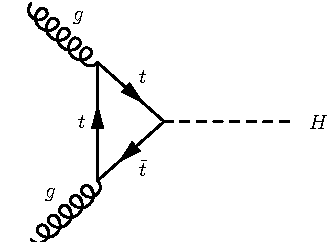
\includegraphics[width=0.3\textwidth]{theoryFigures/ggH.pdf}}
  \subfloat[]{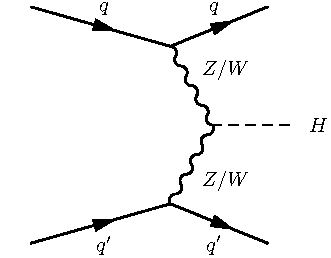
\includegraphics[width=0.3\textwidth]{theoryFigures/vbf.pdf}}\\
  \subfloat[]{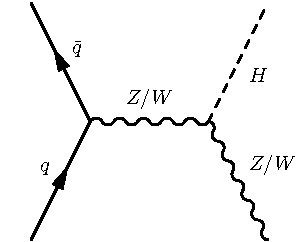
\includegraphics[width=0.3\textwidth]{theoryFigures/wzH.pdf}}
  \subfloat[]{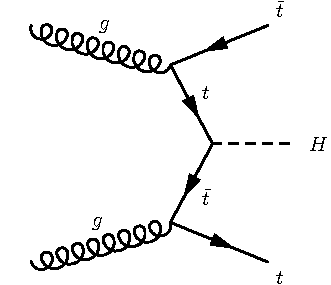
\includegraphics[width=0.3\textwidth]{theoryFigures/ttH.pdf}}
  \caption{Higgs production modes at the LHC: (a) gluon-gluon fusion, via a loop of top quarks, (b) vector boson fusion (VBF), with associated quark production, (c) associated vector boson production and (d) top quark fusion with associated top quark production. }
  \label{fig:theory:higgsproduction}
  \end{figure}

  \newpage
  By the same token, the SM Higgs boson decays to pairs of particles with branching ratios proportional to the square of their mass. The production of a pair of $t$ quarks is not kinematically allowed because their mass is high, so the most likely decay modes are $H \rightarrow ZZ \text{, } W^{\pm}W^{\mp}$, $ b\bar{b}$ and $ \tau^+ \tau^-$. In addition, a small fraction of decays of the Higgs boson ($<1\%$, see Fig. \ref{H_BR_fig}) can occur via a loop diagram to a pair of high-energy photons. The branching fractions and cross sections of these production and decay modes are available in the Handbook of LHC Higgs Cross Sections~\cite{H_XS1,H_XS2}.


  The Higgs boson was discovered in 2012 using data from runs at $\sqrt{s}=7$ and $8$ TeV, and was found to have a mass $m_H \sim 125$ GeV. The signal strengths of the various decay modes at the CMS and ATLAS experiments can be seen in Fig. \ref{sig_strength}. Despite fewer than $1\%$ of Higgs boson decays occurring via $H \rightarrow \gamma \gamma$, this channel played a crucial role in the discovery, and remains one of the two most sensitive methods of studying the Higgs boson. This is in part thanks to the excellent performance of the CMS and ATLAS ECALs, which were able to reach similar sensitivities to the $H\rightarrow \gamma \gamma$ decay mode.

  \subsection{History of Higgs boson searches}
  \subsection{Higgs boson at the LHC}

  \chapter{Overview of the LHC and CMS}
\label{chap:detector}
\section{The Large Hadron Collider (LHC)}
\label{sec:lhc}
%The \LHC~\cite{LHC_machine} is a synchrotron of circumference 27\km, currently the largest and most powerful in the world, installed in the tunnel which previously contained the \LEP~\cite{lepdesign} collider at \CERN. 
The \LHC~\cite{LHC_machine} is currently the largest and most powerful synchrotron in the world, and is installed in the tunnel which previously contained the \LEP~\cite{lepdesign} collider at \CERN. 
The tunnel is located roughly 100\m underground near Geneva, on the border between Switzerland and France. The LHC was designed to perform collisions of two types: \pp (proton-proton) collisions and, less frequently, heavy ion collisions, for example \PbPb (lead-lead). The former is used to search for new particles and perform \SM measurements, such as the ones presented in this thesis. The latter is used, for example, for studies of quark-gluon plasma, and is not discussed in detail here. 

The \LHC is the last stage in a series of machines which form the \CERN accelerator complex, which is illustrated in \Fig~\ref{fig:accelerators}. The procedure by which particles are accelerated using this chain of machines is described in~\cite{LHC_machine}, and is summarised below. In \pp collisions, protons are first obtained from a hydrogen gas, which is stripped of electrons. The particles are then brought up to an energy of 50\MeV using \LINACTWO. The particles coming out of the initial linear accelerator are transfered into the \Booster, which raises the beam energy to 1.4\GeV, before the beams enter the \PS. At this stage, the protons energies are increased to 25\GeV. Once the beams reach the required energy, they are passed into the \SPS, and boosted to 450\GeV. Finally, the beams are injected into the LHC rings, which are two concentric beampipes within the same set of bending magnets. The LHC then brings the beams up to their final energy, which, in the most recent run, was approximately 6.5\TeV, leading to a centre-of-mass collision energy of $\sqrt{s}=13\TeV$. A further increase in the beam energy is foreseen in the \LHC programme, which would bring it up to its design value of 7\TeV per beam, and $\sqrt{s}=14\TeV$.

\begin{figure}[h]
\centering
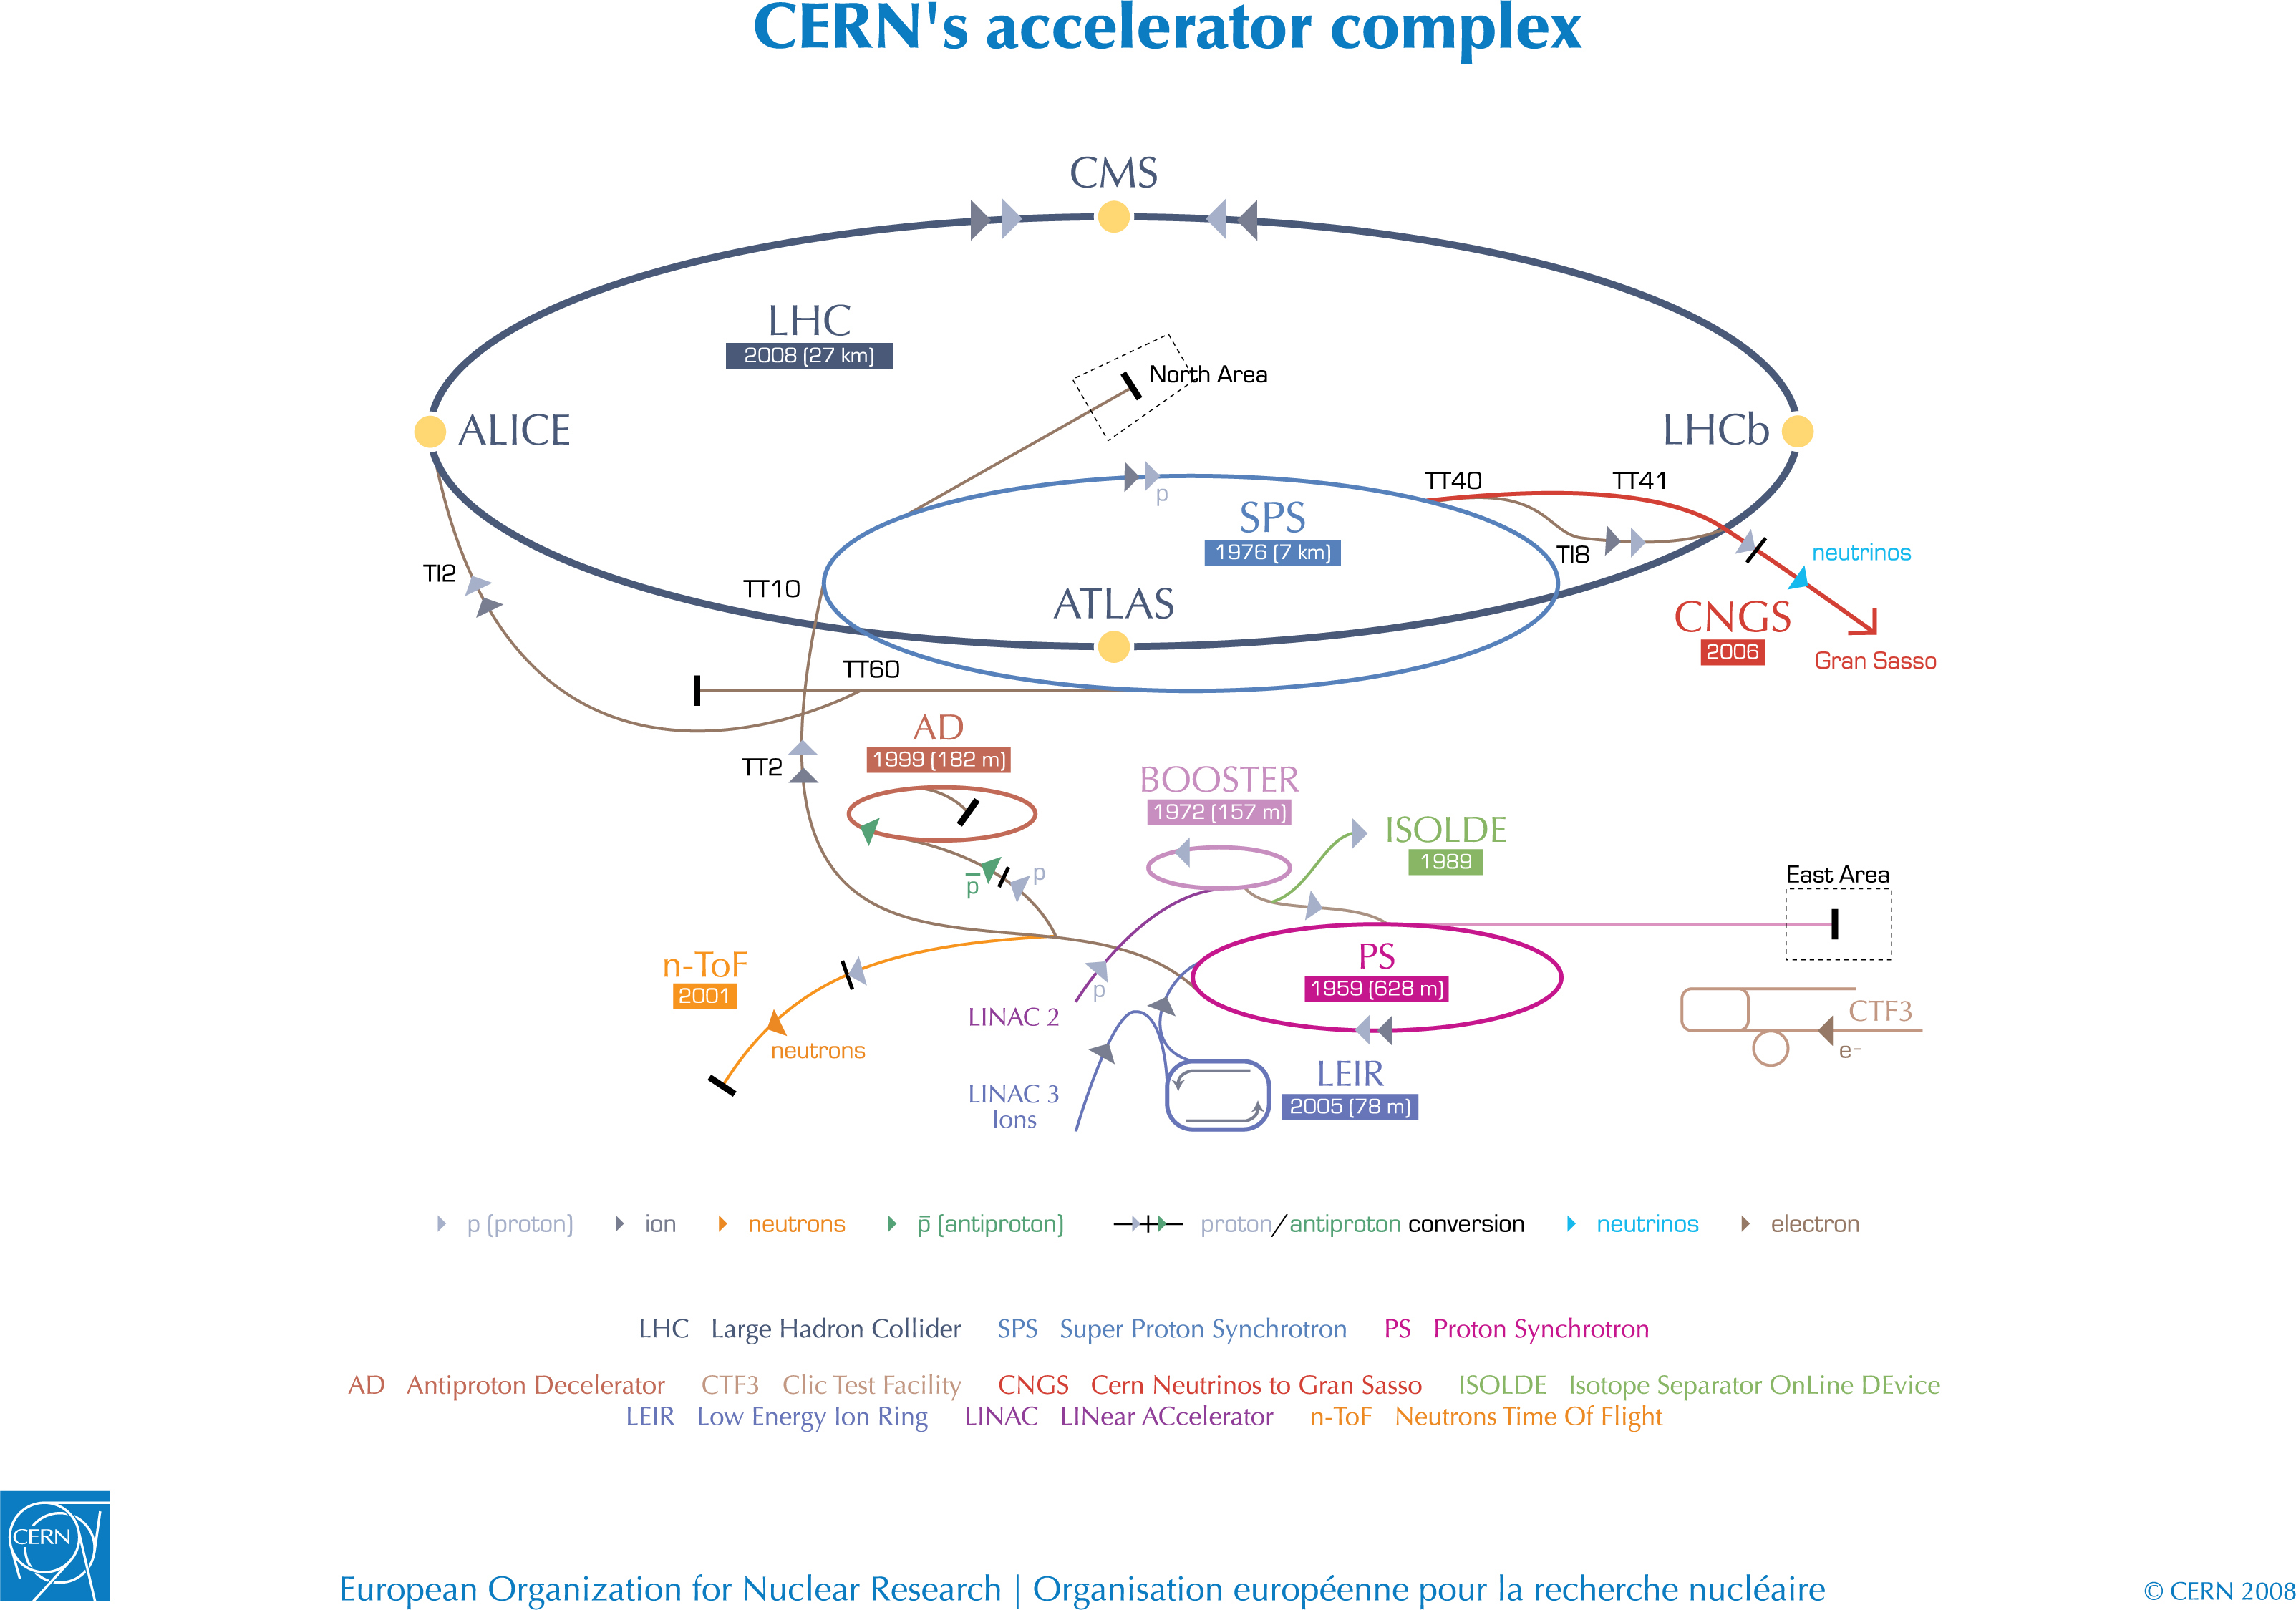
\includegraphics[width=1.0\textwidth]{detectorFigures/accelerators.jpg}
\caption{Schematic view of the CERN accelerator complex, showing the chain of machines which allow the energies of the particles to increase to 6.5\TeV: LINAC2, PS Booster, PS, SPS and finally LHC.~~\cite{Christiane:1260465}}
\label{fig:accelerators}
\end{figure}

The counter-circulating beams in the \LHC are bunched, with each bunch containing several billion protons. The bunch spacing was 50\ns in the initial running of the \LHC, but has now been reduced to its design value of 25\ns, to allow a faster accumulation of data. The average number of times a process occurs in collision experiments ($N_{\text{process}}$) can be obtained from the following relation~\cite{Benedikt:823808}:

\begin{equation}
\label{eq:NeqSigmaL}
N_{\text{process}} = \sigma_{\text{process}}\times \mathcal{L}_{\text{int}},
\end{equation}

where $\sigma_{\text{process}}$ is the \crosssection of the process and $\mathcal{L}_{\text{int}}$ is the integrated luminosity, which is the time integral of the instantaneous luminosity $L$. The luminosity depends only on the machine parameters, and assuming a Gaussian beam distribution, is given by the relation~\cite{Benedikt:823808}:
\begin{equation}
\label{eq:NeqSigmaL}
L = \frac{n_{b} N^{2}_{b} f_{\text{rev}} \gamma_{r}}{4 \pi \epsilon_{n} \beta^{*}} F,
\end{equation}
where $n_{b}$ is the number of bunches in each beam, $N_{b}$ is the number of particles per bunch, $f_{\text{rev}}$ is the revolution frequency, $\gamma_{r}$ is the relativistic gamma factor, $\epsilon_{n}$ is the normalised transverse beam emittance, $\beta^{*}$ is the beta function at the collision point and $F$ is a luminosity reduction factor which takes into account the fact that beams cross at a slight angle. 

The \LHC began operation at $\sqrt{s}=7\TeV$ in 2010, collecting 44\ipb of data in 2010 and 6.1\ifb in 2011. In 2012, the collision energy was successfully increased to $\sqrt{s}=8\TeV$ and 23.3\ifb of data were recorded. This period corresponded to the first physics run of the \LHC (\RunI). After a shutdown period for planned upgrades to the machine, the \LHC began \RunII and raised its collision energy to $\sqrt{s}=13\TeV$, delivering 4.3\ifb in 2015 and \totaldatatwentysixteen\ifb in 2016, as can be seen in \Fig~\ref{fig:totalintlumi}. 
\ifNewAnalysis
The analysis of the full 2016 dataset is presented in this thesis.
\else
The analysis of the first \thisanalysislumi\ifb collected in 2016 is presented in this thesis.
\fi
The peak instantaneous luminosity of the \LHC, achieved at the start of periods of colliding beams, is currently around $1.4 \times 10^{34}$\lumiunits, significantly exceeding the design luminosity of $1 \times 10^{34}$\lumiunits. \RunII is scheduled to continue until 2018 before another shutdown for upgrades is envisaged. 

\begin{figure}[h]
\centering
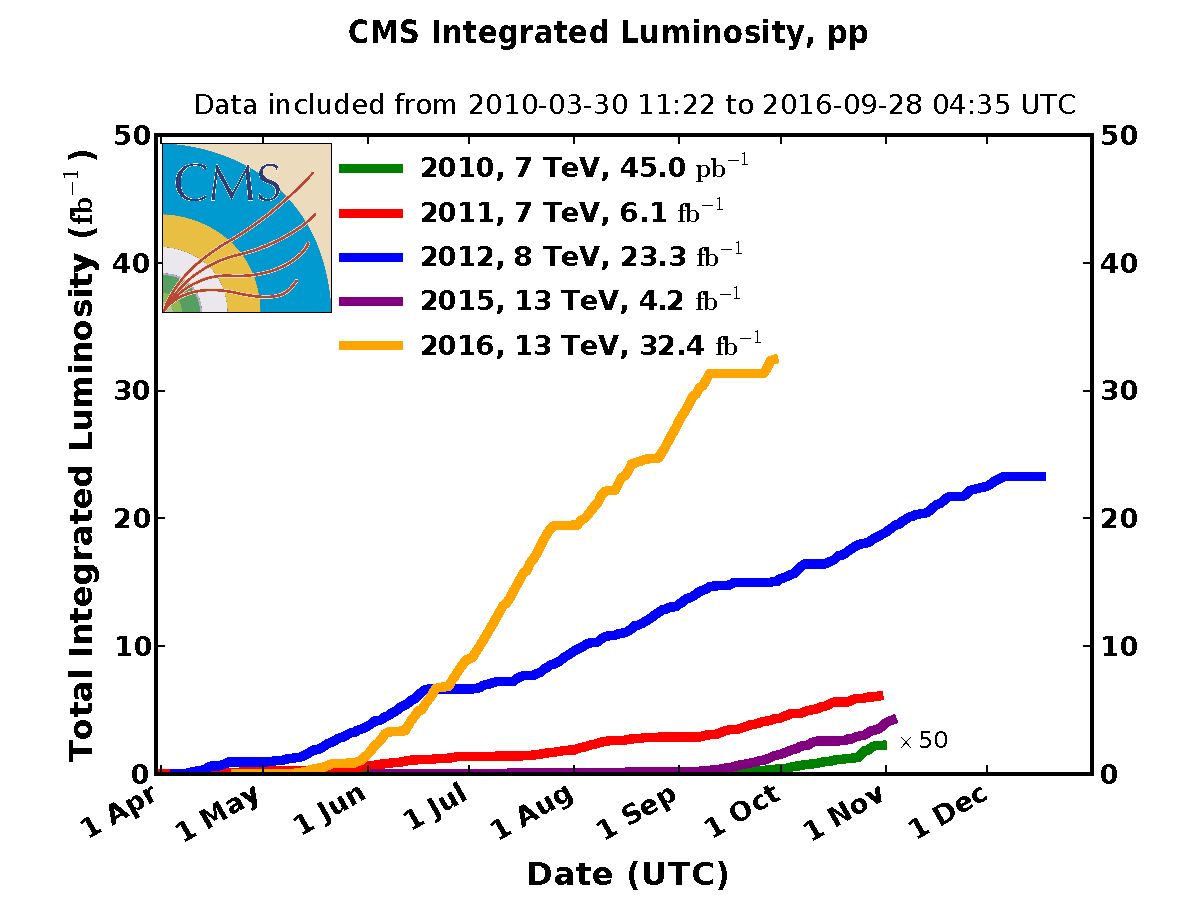
\includegraphics[width=1.0\textwidth]{detectorFigures/int_lumi_cumulative_pp_2_280916.pdf}
\caption{Overview of the integrated luminosity delivered by the LHC throughout its operation until the time of writing, as recorded by CMS.~~\cite{CMSLumiPublic}}
\label{fig:totalintlumi}
\end{figure}

There are eight points along the \LHC ring which are equipped with access shafts, as well as surface and underground structures. Four of these points host \LHC infrastructure elements: the collimators at points 3 and 7, the RF system at point 4 and the beam dump at point 6. The remaining four points house experimental caverns where beams are focused and brought into collision. Two general purpose detectors are located at diametrically opposed sides of the ring: \ATLAS~\cite{AtlasatLHC} at point 1 and \CMS~\cite{CMSatLHC} at point 5. Two additional specialised detectors are located at points 2 and 8, namely \ALICE~\cite{AliceatLHC} (used in the study of heavy ion collisions) and \LHCb~\cite{LHCbatLHC} (specialising in flavour physics) respectively. 



\section{The Compact Muon Solenoid (CMS)}
\label{sec:cms}

\subsection{Overview}
\label{sec:cms:overview}

\CMS is located approximately 100\m underground at access point 5 of the \LHC, near the French village of Cessy. It is over 21\m long and 14\m in diameter, weighing over 12,500 tons. It consists of a superconducting solenoid magnet 13\m long and 5.9\m in diameter, generating a 3.8\T magnetic field, which is embedded within an iron return yoke containing the muon detection system. The other sub-detectors are contained within the solenoid. The layout of the \CMS detector can be seen in \Fig~\ref{fig:cms-exploded}. \CMS is composed of a cylindrical barrel region closed by two endcaps. The tracker (described in \Sec~\ref{sec:cms:tracker}), \ECAL (described in \Sec~\ref{sec:cms:ecal}), and \HCAL (described in \Sec~\ref{sec:cms:hcal}) are housed within the solenoid. Outside of the solenoid, four layers of iron act as a return yoke for the magnet and house muon detector chambers (described in \Sec~\ref{sec:cms:muondetector}). 

The \LHC experiments use a right-handed coordinate system whereby the $x$-axis points towards the centre of the \LHC ring, the $y$-axis points upwards, and the $z$-axis points in the direction of the counter-clockwise beam. A more convenient coordinate system can be defined for physics analyses using the variables $(\eta,\phi,z)$. In this convention, $\eta = -\ln [ \tan(\theta/2)]$ is the pseudorapidity (where $\theta$ is the polar angle relative to the beam axis) and $\phi$ is the angle relative to the $x$-axis in the $(x,y)$ plane. The direction perpendicular to the $z$-axis is referred to as \emph{transverse}, while the direction pointing along it is referred to as \emph{longitudinal}. The transverse components of energy and momentum are denoted by \ET and \pT respectively. 

%Each instance where the data from a bunch crossing are saved by the detector is known as an event. Typically, an event will have a single interaction which is of interest. At 13\TeV the \pp interaction \crosssection is very large, so several interactions per crossing are expected. The physical locations of these interactions are referred to as vertices, with the interaction of interest occurring at the \PV, and other interactions at secondary vertices. The additional interactions in an event, other than the one occurring at the \PV, are collectively referred to as \PU. 

\begin{figure}[h]
\centering
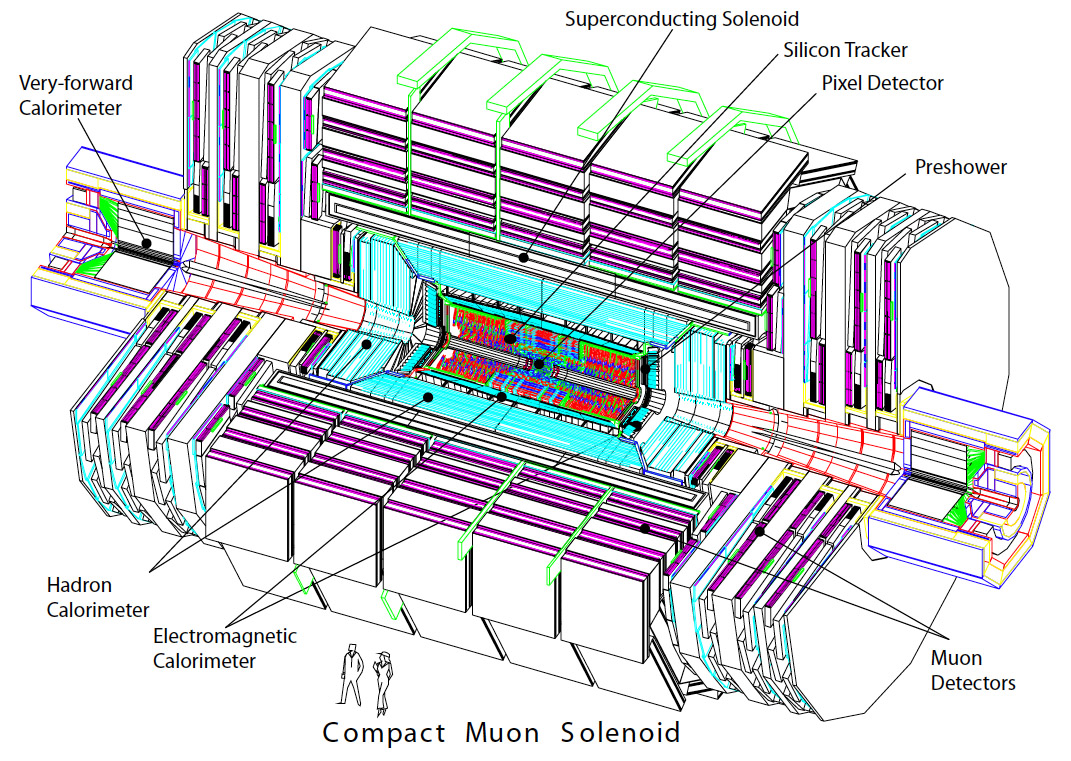
\includegraphics[width=1.0\textwidth]{detectorFigures/cms-perspective.png}
\caption{A cutaway diagram of the CMS detector, showing the main components and subdetectors, which are described in \Sec~\ref{sec:cms}~\cite{CMSTDR}.}
\label{fig:cms-exploded}
\end{figure}

\subsection{Tracker}
\label{sec:cms:tracker}

The closest \subdetector to the beam crossing point is the tracker~\cite{CMSTrackerTDR}, the layout of which can be seen in \Fig~\ref{fig:trk}. This \subdetector, which fits within a cylindrical volume 5.8\m long and 2.5\m in diameter, is used to measure the momenta of charged particles whose tracks are deflected in the 3.8\T magnetic field. 
The short interval between collisions (25\ns) requires the tracker to have a fast response time. Furthermore, the large \pp \crosssection necessitates it to be resistant to radiation. The two requirements are satisfied by silicon-based detectors. Two silicon detector types are used in the \CMS tracker: the pixel layers and the silicon strip layers.

%The barrel section of the tracker comprises three cylindrical layers of silicon pixel detectors close to the interaction region, surrounded by ten layers of silicon strip detectors. The endcaps consist of two discs of silicon pixel detectors and twelve discs of silicon strip detectors. Momenta of charged particles can be determined by measuring the curvature of tracks as they bend in the strong magnetic field. For tracks of \pT of the order of 100\GeV, the \pT resolution of the tracker is between 1.5\% and 2.5\%. %% repeated information


\begin{figure}[h]
\centering
\includegraphics[width=1.0\textwidth]{detectorFigures/trackerSchematic.png}
\caption{A diagram showing the layout of the CMS tracker components: the pixel tracker (labelled PIXEL) is the nearest to the interaction region marked by the black dot. The various sections of the strip tracker (TIB, TID, TOB, TEC$+$ and TEC$-$) are arranged around the pixel tracker. \cite{CMSTDR}}
\label{fig:trk}
\end{figure}

The pixel layers are made up of 66 million 100\um $\times$ 150\um silicon pixels. As can be seen in \Fig~\ref{fig:trk}, these are arranged into three concentric cylinders in the barrel section (of radii between 4.4\cm and 10.2\cm) and two planes on each endcap. The spatial resolution of this part of the tracker is around 10\um in the transverse direction. The pixel layers also have excellent longitudinal resolution (20-40\um), which is important for vertex reconstruction.~\cite{trackerperformance2014}

The silicon strip layers surround the pixel layers, and are composed of several sections. Four cylindrical layers form the tracker inner barrel (TIB), while the tracker inner disks (TID) are composed of three planes. Surrounding this, the tracker outer barrel (TOB) provides a further 6 cylindrical layers, while 9 planes form the tracker endcaps (TEC). The silicon strip layers extend to 110\cm in radius. This section of the tracker uses 9.3 million strips, with each strip being 10-20\cm long and 80-183\um wide. The transverse spatial resolution of the silicon strip layers is between 13-38\um in the inner section and 18-47\um in the outer section.~\cite{trackerperformance2014}

Charged particles follow helical trajectories in the \CMS magnetic field, and deposit charge as they pass through the silicon sensors. The resulting recorded signals are referred to as hits. Using multiple hits in the pixel and strip detectors, the helical trajectory can be reconstructed. The transverse momentum \pT of charged particles can then be extracted from the curvature of the helix. The \pT resolution is of the order of 2-3\% in the $|\eta|<1.6$ region and up to 11\% for the outer section. Using the extrapolation from the fitted track and the longitudinal resolution of the pixel detector, tracks are grouped into common points of origin, at the \PV and secondary vertices. 

\subsection{Electromagnetic Calorimeter}
\label{sec:cms:ecal}

The \ECAL~\cite{CMSTDR,CMSEcalTDR} is the \subdetector whose performance is the most critical to the \Hgg analysis, and its layout, operation and calibration will therefore be described in some detail. 

\subsubsection{ECAL overview}
\label{sec:cms:ecal:overview}

The \ECAL is made up of an array of 61,200 lead tungstate (PbWO$_4$) crystals in the barrel section and 14,648 crystals in the endcaps, arranged one crystal deep. The choice of material was made because PbWO$_4$ has a short radiation length (the mean distance over which an electron loses all but $1/e$ of its energy to bremsstrahlung) of 0.89\cm. The short radiation length is important in the \ECAL design because it allows electromagnetic showers to be contained within a relatively small depth of material. 
%and a small Moli\`ere radius (the radius of a cylinder containing on average 90\% of a shower's energy) of 1.96\cm. It is also a fast scintillator and radiation resistant. These crystal properties are a central feature of the \CMS detector as it allows excellent energy resolution of incoming photons. 

The \ECAL crystal front faces are 22\mm $\times$ 22\mm squares, corresponding to approximately $\Delta \eta \times \Delta \phi = 0.0174 \times 0.0174$, roughly matching the Moli\`ere radius of PbWO$_4$. The individual crystal depth is approximately 26 radiation lengths, to ensure that the electromagnetic showers are fully contained within the \ECAL. The array of crystals extends to $|\eta| = 3$, but precision measurements are only made up to $|\eta| =2.5$. There are also transition regions between the ECAL barrel and endcaps around $|\eta| = 1.5$. The arrangement of the crystals in the \ECAL can be seen in \Fig~\ref{fig:ecal}.

\begin{figure}[h]
\centering
\includegraphics[width=1.0\textwidth]{detectorFigures/ecalEBEE.png}
\caption{Schematic \crosssection of one quadrant of the ECAL, showing the arrangement of crystals in the ECAL barrel and endcaps \cite{CMSEcalTDR}. The shower detector (SE, referred to as ES in the text) is also visible, as is the hadron calorimeter barrel (HB) and the tracker (TK).}
\label{fig:ecal}
\end{figure}


%Radiation exposure at the level expected at the LHC does not affect the scintillation mechanism of the crystals.




%\begin{figure}[h]
% \centering
%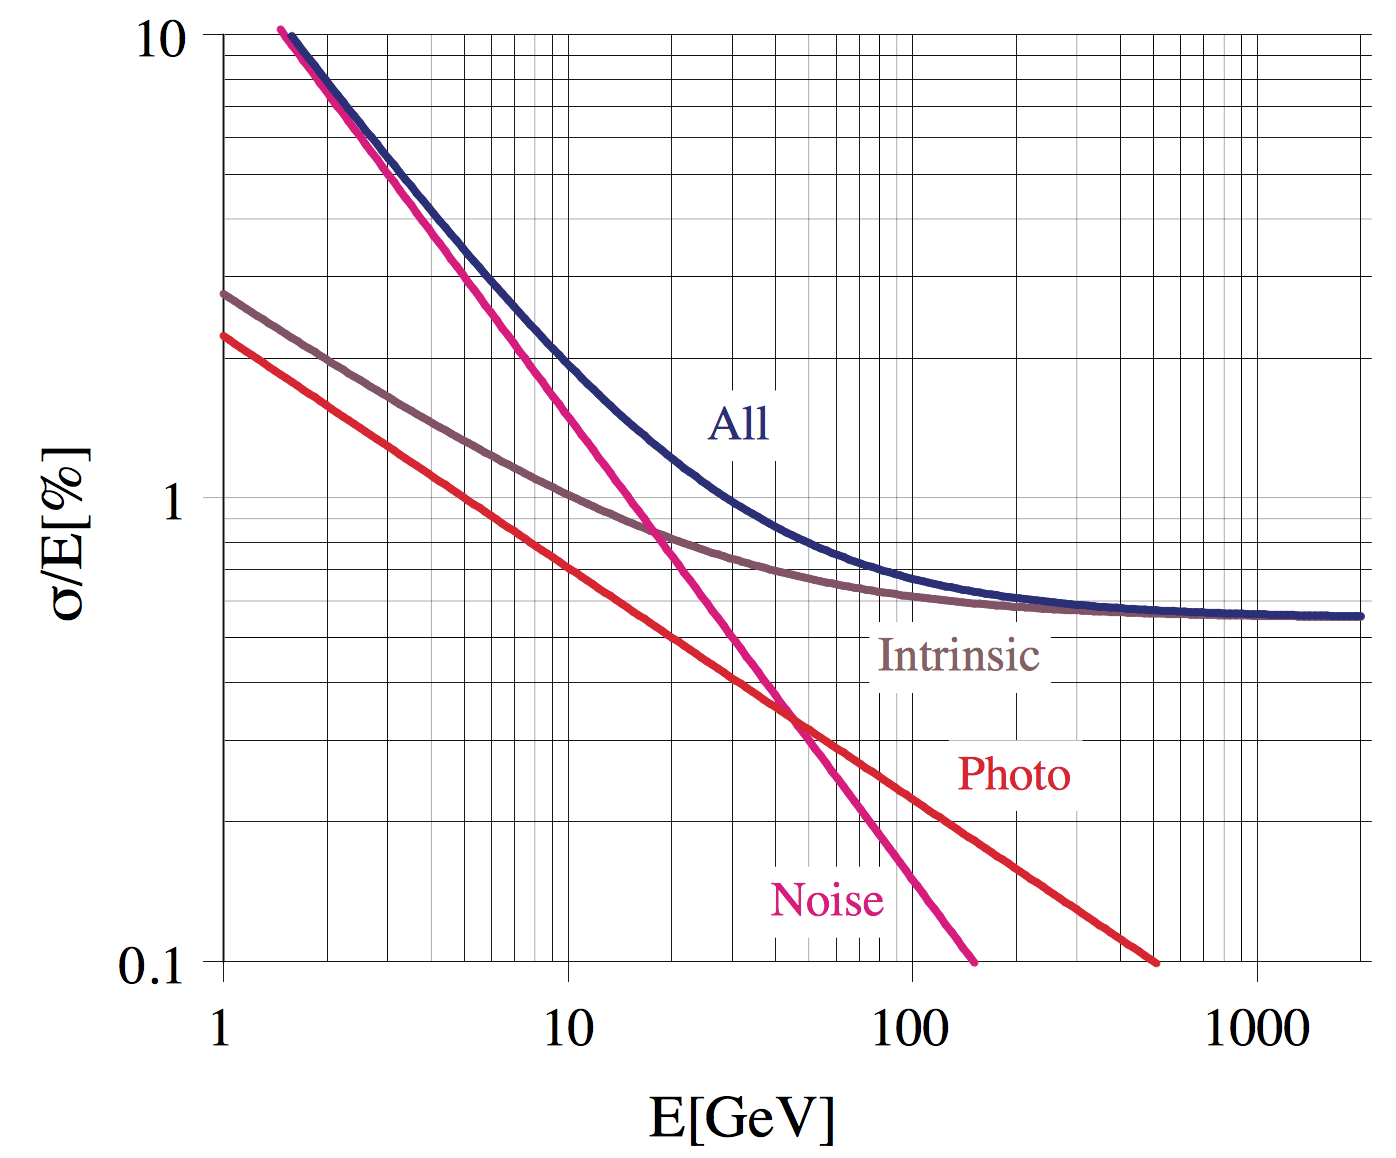
\includegraphics[width=0.6\textwidth]{detectorFigures/EcalResolutionParametrisation.png}
% \caption{The different contributions to the ECAL energy resolution The blue line represents the sum of the stochastic term (red line), the noise term (pink line) and the constant term plus corrected for shower containment (violet line).~\cite{CMSEcalTDR}}
%\label{fig:ecal:resol}
%\end{figure}


The \ECAL consists of the \EB and the \EE. The \EB provides coverage in the region $|\eta| < 1.479$, while the \EE provides coverage for $1.556 < |\eta| < 2.5$. The crystals in the \EB are grouped into 36 supermodules, each covering an angle of $20^o$ in $\phi$. The crystals are arranged so that they do not point directly at the mean position of the primary interaction vertex, but are instead positioned with a $3^o$ offset in both $\theta$ and $\phi$, to help improve the hermeticity of the detector. The \EE is composed of two ``D''-shaped sections, built up of \emph{supercrystals} (units of 25 standard crystals). The \EE has notably worse resolution that the \EB, and this is because the calibration of the crystals is more challenging. One factor contributing to this is that the crystal transparency is affected by the high radiation doses in the \EE. %Another is that the crystal faces in units of $\eta,\phi$ are larger in the \EE than the \EB, and since the energy deposited by additional interactions in a collision, \PU, is roughly constant in unit areas of $\eta,\phi$, the \EE crystals have to deal with more noise.

An additional detector, the \ES, is mounted in front of each endcap, covering the region $1.54 <|\eta| < 2.61$. The main purpose of which is to distinguish between $\pi^0$ and $\gamma$ particles, and also adds three radiation lengths to the depth of the \ECAL endcaps. The \ES is composed of two planes of lead, of 2 and 1 radiation lengths respectively, with high granularity silicon detector strips after each. %The \ES is used to identify $\pi^0\rightarrow \gamma \gamma$ photons, where both photons strike the same crystal. This is possible because the \ES has a much finer granularity than the \EE, so a prompt photon will register in just one strip of the \ES, while a pion decaying to two photons registers in two strips. Although the \EE might interpret $\pi^0\rightarrow \gamma \gamma$ as one highly energetic photon, the high granularity of the silicon strips in the \ES allow two tracks to be identified. 

In the barrel region, \APDs operating with a gain of 50, are attached to the back of the crystals, where the scintillation light is collected. In the endcaps, \VPTs are used instead of \APDs as the photo-detectors. In both cases, the photo-detectors register $\sim 4000 $ photoelectrons per \GeV. The photo-detectors are read out by 12-bit \ADC. Ten consecutive samples are read out and stored for each crystal, and this information is used to determine the amplitude of the pulse, and therefore the amount of energy deposited in the crystal.

The resolution of the \ECAL crystals is modelled with the following equation:
\begin{equation} 
\left( \frac{\sigma}{E}\right) ^2= \left( \frac{S}{\sqrt{E}} \right)^2 + \left( \frac{N}{E} \right)^2 + C^2,
\end{equation}
where $S$ represents the stochastic term, $N$ represents the noise term and $C$ represents a constant term~\cite{CMSTDR}. The design values of these parameters are approximately $S=2.8\%$ GeV$^\frac{1}{2}$, $ N= 0.12$ GeV and $C=0.3 \%$. 

As can be seen in \Fig~\ref{fig:det:energy_resol}, for individual \Hgg photons in \RunI, an energy resolution of about 1\% was achieved for unconverted photons in the barrel, and about 2.5\% in the endcaps. For converted photons, an energy resolution of about 1.3\% was observed up to $|\eta| = 1$, rising to about 2.5\% at $|\eta| = 1.4$, and 3-4\% in the endcaps~\cite{CMS-PAS-EGM-14-001}.

\begin{figure}[h]
\centering
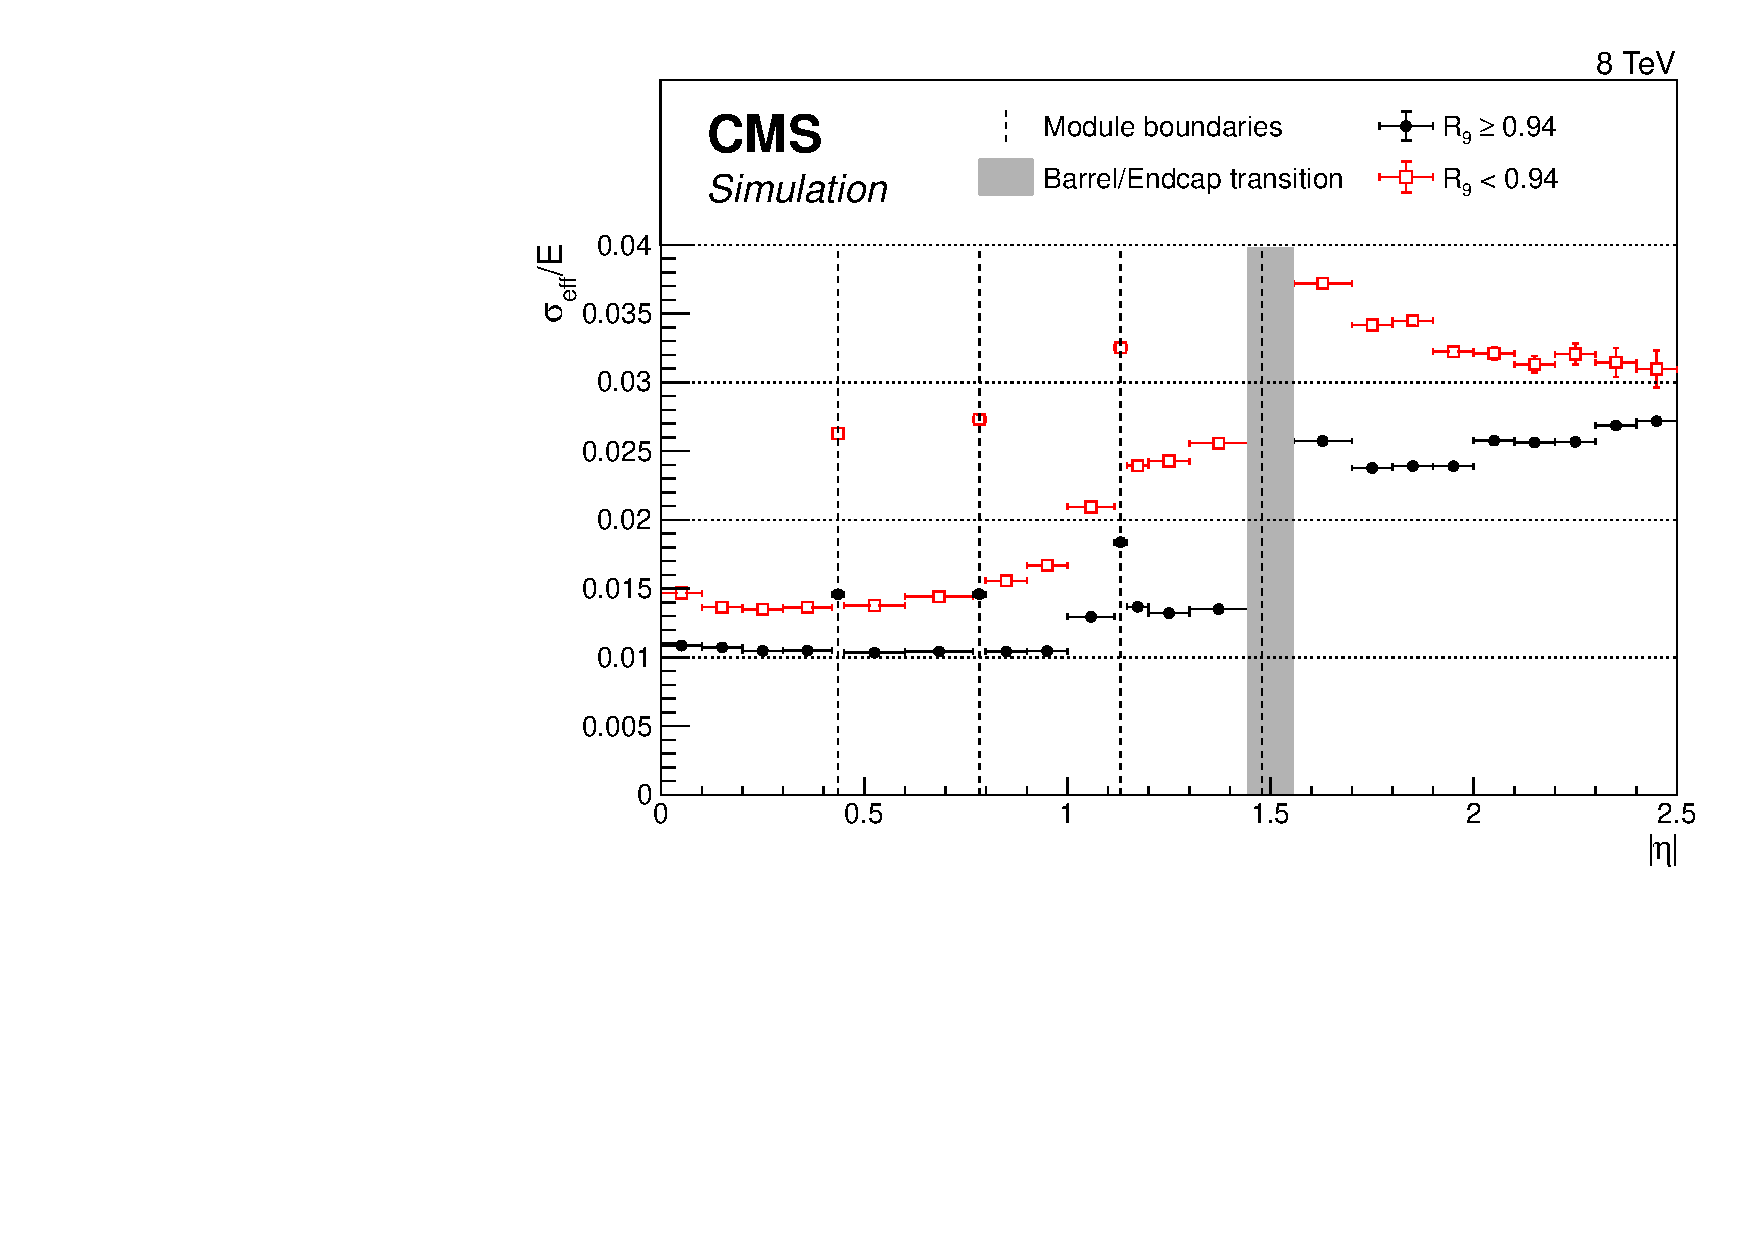
\includegraphics[width=0.8\textwidth]{detectorFigures/effSigma_vs_Eta_mva.pdf}
\caption{The relative energy resolution of individual simulated \Hgg photons in \RunI as a function of $|\eta|$, shown separately for converted photons (black circles) and unconverted photons (open red squares). The vertical lines represent the boundaries between the ECAL modules in the barrel, while the grey band indicates the transition region between the EB and the EE, where photons are not reconstructed \cite{CMS-PAS-EGM-14-001}.}
\label{fig:det:energy_resol}
\end{figure}

\subsubsection{Energy measurement}
\label{sec:cms:ecal:energymeasurement}

Typically, energy deposits will not be contained in a single crystal. When an electron or a photon hits the \ECAL, the electromagnetic shower will spread out into adjoining crystals. In addition, particles can undergo pair conversion or emit bremsstrahlung before impacting the detector, resulting in additional associated energy deposits.
%photons travelling towards the \ECAL can interact with the tracker material and undergo pair conversion, resulting in two nearby or overlapping showers. Furthermore, electrons or positrons travelling towards the \ECAL will be deflected in the $\phi$-direction by the magnetic field, and will emit photons via bremsstrahlung: in this case the radiated photons will make subsequent deposits in the \ECAL. 
Clustering algorithms are used to recover the deposits from the main impact crystal, adjacent crystals where the energy from the main shower is spread out, and the additional associated crystals, and group them into a so-called \SC. %The algorithm by which this is achieved is described in \Sec~\ref{sec:obj:egamma:clustering}. 
The energy of the \SC ($E_{\textrm{SC}}$) can roughly be expressed as: 

\begin{equation} 
\label{eq:cms:ecal:energy}
E_{\text{SC}} = F_{\text{SC}} \cdot G \cdot \Sigma^{i=0}_{N_\text{crystals}} ( C_{i} \cdot S_{i}(t) \cdot A_{i}) ,
\end{equation}
where $F_{\text{SC}}$ is a correction to the \SC energy sum representing second-order effects, $G$ is an ADC-to-GeV conversion factor which represents the global energy scale, $C_{i}$ is a factor applied to crystal $i$ to equalise the response (also known as an intercalibration constant), $S_{i}(t)$ is a time-dependent factor to correct for loss of transparency of the crystals, and $A_{i}$ is the amplitude of the pulse recorded in that crystal for the bunch crossing in question. In regions covered by the \ES, the signals from this \subdetector are also used.~\cite{cmsEcalCalibration}


\subsubsection{Calibration}
\label{sec:cms:ecal:calibration}

The calibration of the \ECAL involves using various techniques and physics objects to tune the values of $S_{i}(t)$, $C_{i}$ and $G$ in \Eq~\ref{eq:cms:ecal:energy}. 

The first step is to make a time-dependent correction for the transparency in the crystals. Indeed, the response of \ECAL crystals varies because of radiation induced transparency loss and recovery through spontaneous annealing. Continuous monitoring and correction of the response of the crystals is required. This is achieved using a laser which periodically (every 40 minutes) injects photons of wavelength 440\nm into each crystal via a network of optical fibres. The change of the response as measured and corrected for using this mechanism is tracked in \Fig~\ref{fig:cms:ecal:lasercorrections}. The effect of the corrections on the measured mass of the $\pi^0$ in its decay to photons can be seen in \Fig~\ref{fig:cms:ecal:pizeroLMcorr}.

\begin{figure}[h]
\centering
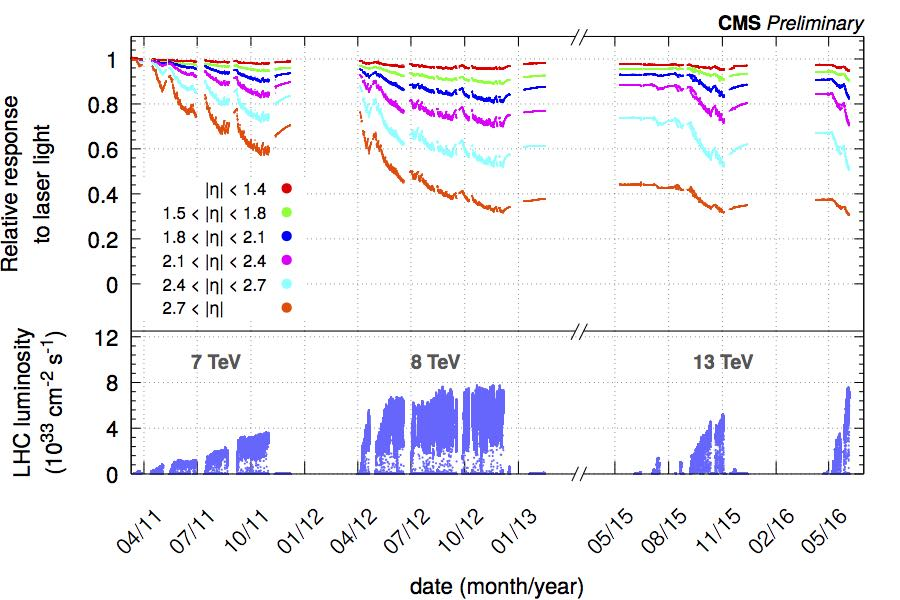
\includegraphics[width=1.0\textwidth]{detectorFigures/EcalLaserCorrections.jpg}
\caption{The response of the CMS ECAL lead tungstate crystals is shown as a function of time, and for different pseudorapidity ranges. The crystal response decreases as data are collected, due to transparency loss caused by exposure to radiation, and recovers during spontaneous annealing at times when no beams are present. \cite{CMSECALPublic}}
\label{fig:cms:ecal:lasercorrections}
\end{figure}

\begin{figure}[h]
\centering
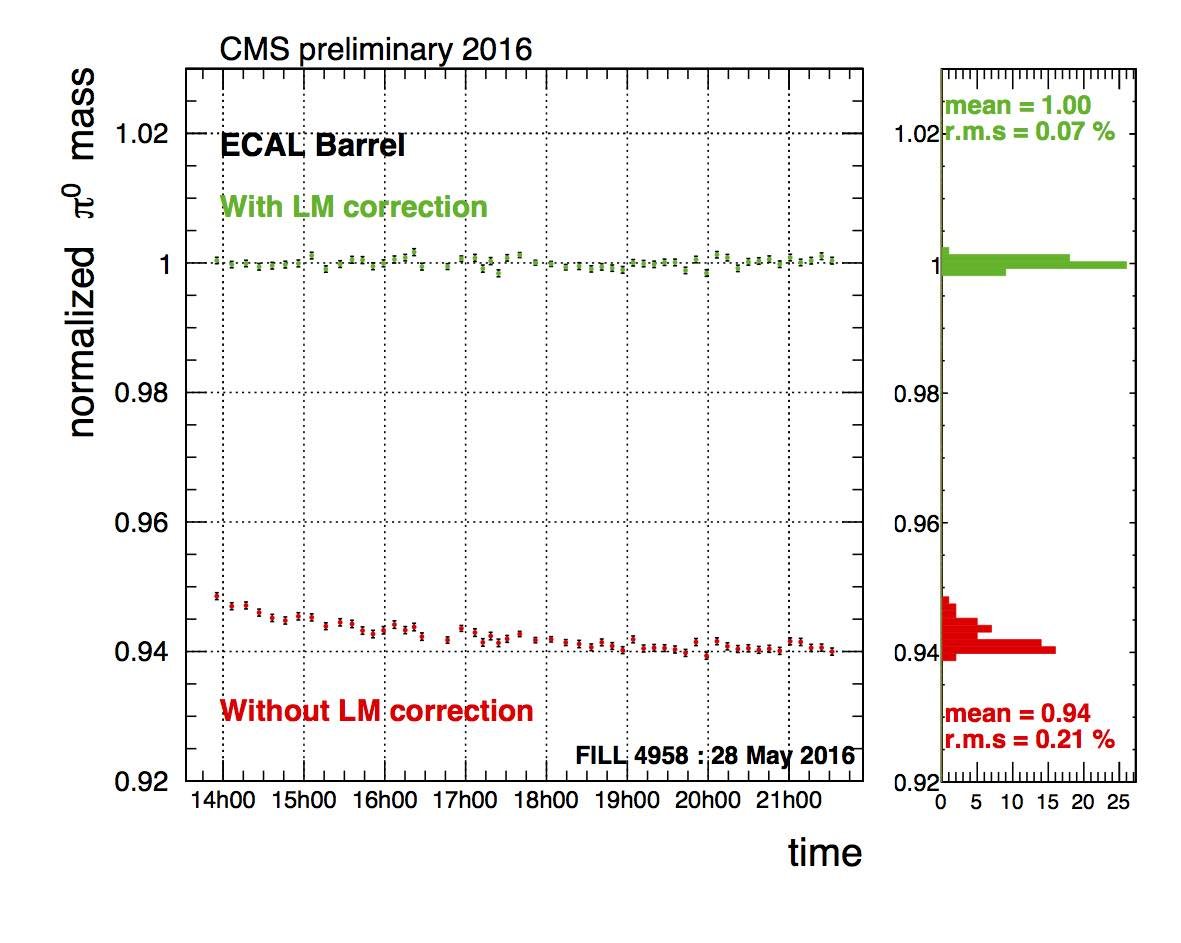
\includegraphics[width=1.0\textwidth]{detectorFigures/pi0_EB_plus_1.jpg}
\caption{The normalised value of the invariant mass of the $\pi^0$ particle in its decay to photons, as measured by the CMS ECAL barrel, with and without the Laser Monitoring (LM) corrections for crystal transparency loss, showing the degradation of the response of the lead tungstate crystals, even over a period of hours. \cite{CMSECALPublic}}
\label{fig:cms:ecal:pizeroLMcorr}
\end{figure}

The next step is the intercalibration, which aims to equalise the response of all crystals. This is achieved by determining a set of intercalibration constants $C_{i}$, one for each crystal. Several methods are used in this procedure. The first is to use the fact that the \CMS \ECAL is cylindrically symmetric. It is therefore expected that during a given period of time, the total energy measured by each crystal with the same value of $\eta$ ($\eta$-ring) should be the same. Exploiting the $\phi$-symmetry of the detector, one can therefore produce an intercalibration constant for each crystal in an $\eta$-ring by dividing the amount of energy that was measured by that crystal in an interval of time by the average amount measured by all crystals in that $\eta$-ring. Another method exploits the fact that the invariant mass of $\pi^0$ or $\eta$ particles (as measured in their decay to photons) should be measured the same regardless of the crystal location. Therefore, one can generate intercalibration constants by dividing the measured values of the invariant masses in each crystal by the average value measured by all crystals. Intercalibration constants produced using different methods are combined to give a final set of per-crystal corrections. By construction, the average value of the intercalibration constants is unity: these corrections leave the overall scale unchanged.

The final step in the calibration procedure is to set the global scale $G$, which is also the ADC-to-GeV conversion factor. This is set by comparing the measured value of the mass of the $\PZ$ boson in its decay to electrons to the nominal value. Since the mass of the $\PZ$ is well known and simulated, one can set the value $G$ such that the peak of the $\PZ$ invariant mass distribution coincides with the simulated value, in different bins of $\eta$ and \SC type, in order to complete the calibration.


\subsection{Hadronic Calorimeter}
\label{sec:cms:hcal}

The \HCAL is used to identify hadrons, and measure their positions and energies. In particular, it is needed to measure the energy of neutral hadrons which do not leave any hits in the tracker or any deposits in the \ECAL. Such particles need to be taken into account to accurately estimate the energies and directions of jets of particles, and to measure the magnitude and direction of any missing energy, which would indicate particles which did not interact by the \CMS detector (e.g.~neutrinos, or undiscovered weakly interacting particles). 

The \CMS \HCAL is a sampling calorimeter, consisting of active material between absorber plates. The layout of the detector can be seed in \Fig~\ref{fig:hcal}. The active material is a plastic scintillator read out by wavelength-shifting plastic fibres. The absorber plates are made of brass (or steel in the forward section). Brass is chosen as it is an non-magnetic material, and thus will not be affected by the strong magnetic field within the solenoid. The main body of the \HCAL is composed of the \HB with coverage up to $|\eta| < 1.3$, and the \HE with coverage up to $|\eta| < 3$, with $\Delta\phi \times \Delta\eta$ granularities between $0.087 \times 0.087$ and $ 0.17 \times 0.17$. In order to accurately measure missing energy, the \HCAL must be as hermetic as possible. For this reason, an additional calorimeter is appended, the \HF, which gives coverage up to $|\eta| <5$. This uses active quartz fibres within a steel absorber matrix. In order to fully contain hadronic showers, an additional component, the \HO, uses the solenoid as an absorber and is placed directly around it in the barrel region.~\cite{cmsHcal} 

\begin{figure}[h]
\centering
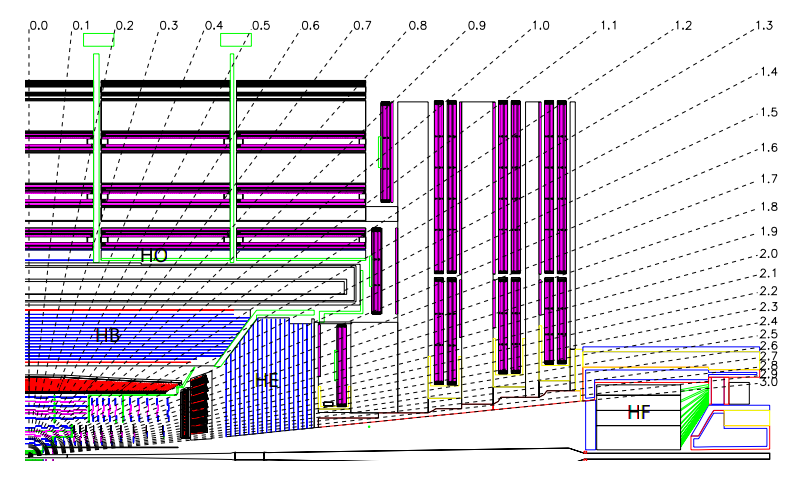
\includegraphics[width=1.0\textwidth]{detectorFigures/cms_hcal.png}
\caption{Schematic \crosssection of one quadrant of the HCAL, showing the arrangement of the various components of the \subdetector: The HB and HE surrounding the ECAL, with the HF at high $\eta$ and the HO just outside of the solenoid \cite{CMSatLHC}.}
\label{fig:hcal}
\end{figure}

The minimum depth of the \HB is 5.8 radiation lengths, rising to 11.8 when the \HO is taken into account. In the endcaps, the depth is at least 10 radiation lengths~\cite{cmsHcal}. The resolution of the \HCAL system was measured in test beams of single pions~\cite{Abdullin:2009zz} and found to be:
\begin{equation}
\label{eq:HCALresol}
\left( \frac{\sigma}{E}\right) ^2= \left( \frac{94.3\%}{\sqrt{E}} \right)^2 + \left( \frac{8.4\%}{E} \right)^2.
\end{equation}

\subsection{Muon detectors}
\label{sec:cms:muondetector}

The solenoid is surrounded by the outermost \subdetector, the muon detector, which is built into and around the steel return yoke for the magnetic field.
The \CMS muon detection system consists of both endcap and barrel sections and is comprised of three types of detector: the \DTs in the barrel, the \CSCs in the endcaps, and the \RPCs in both barrel and endcaps. The muon chambers are all installed between the layers of the steel return yoke. The layout of the muon detectors can be seen in \Fig~\ref{fig:muonssystem}. All the muon detectors are gaseous detectors with a similar operational principle: as charged particles travel through a chamber, the gas contained within becomes ionised and the resulting electrons drift towards the detector's anode, which gives out an electric signal. 
\begin{figure}[h]
\centering
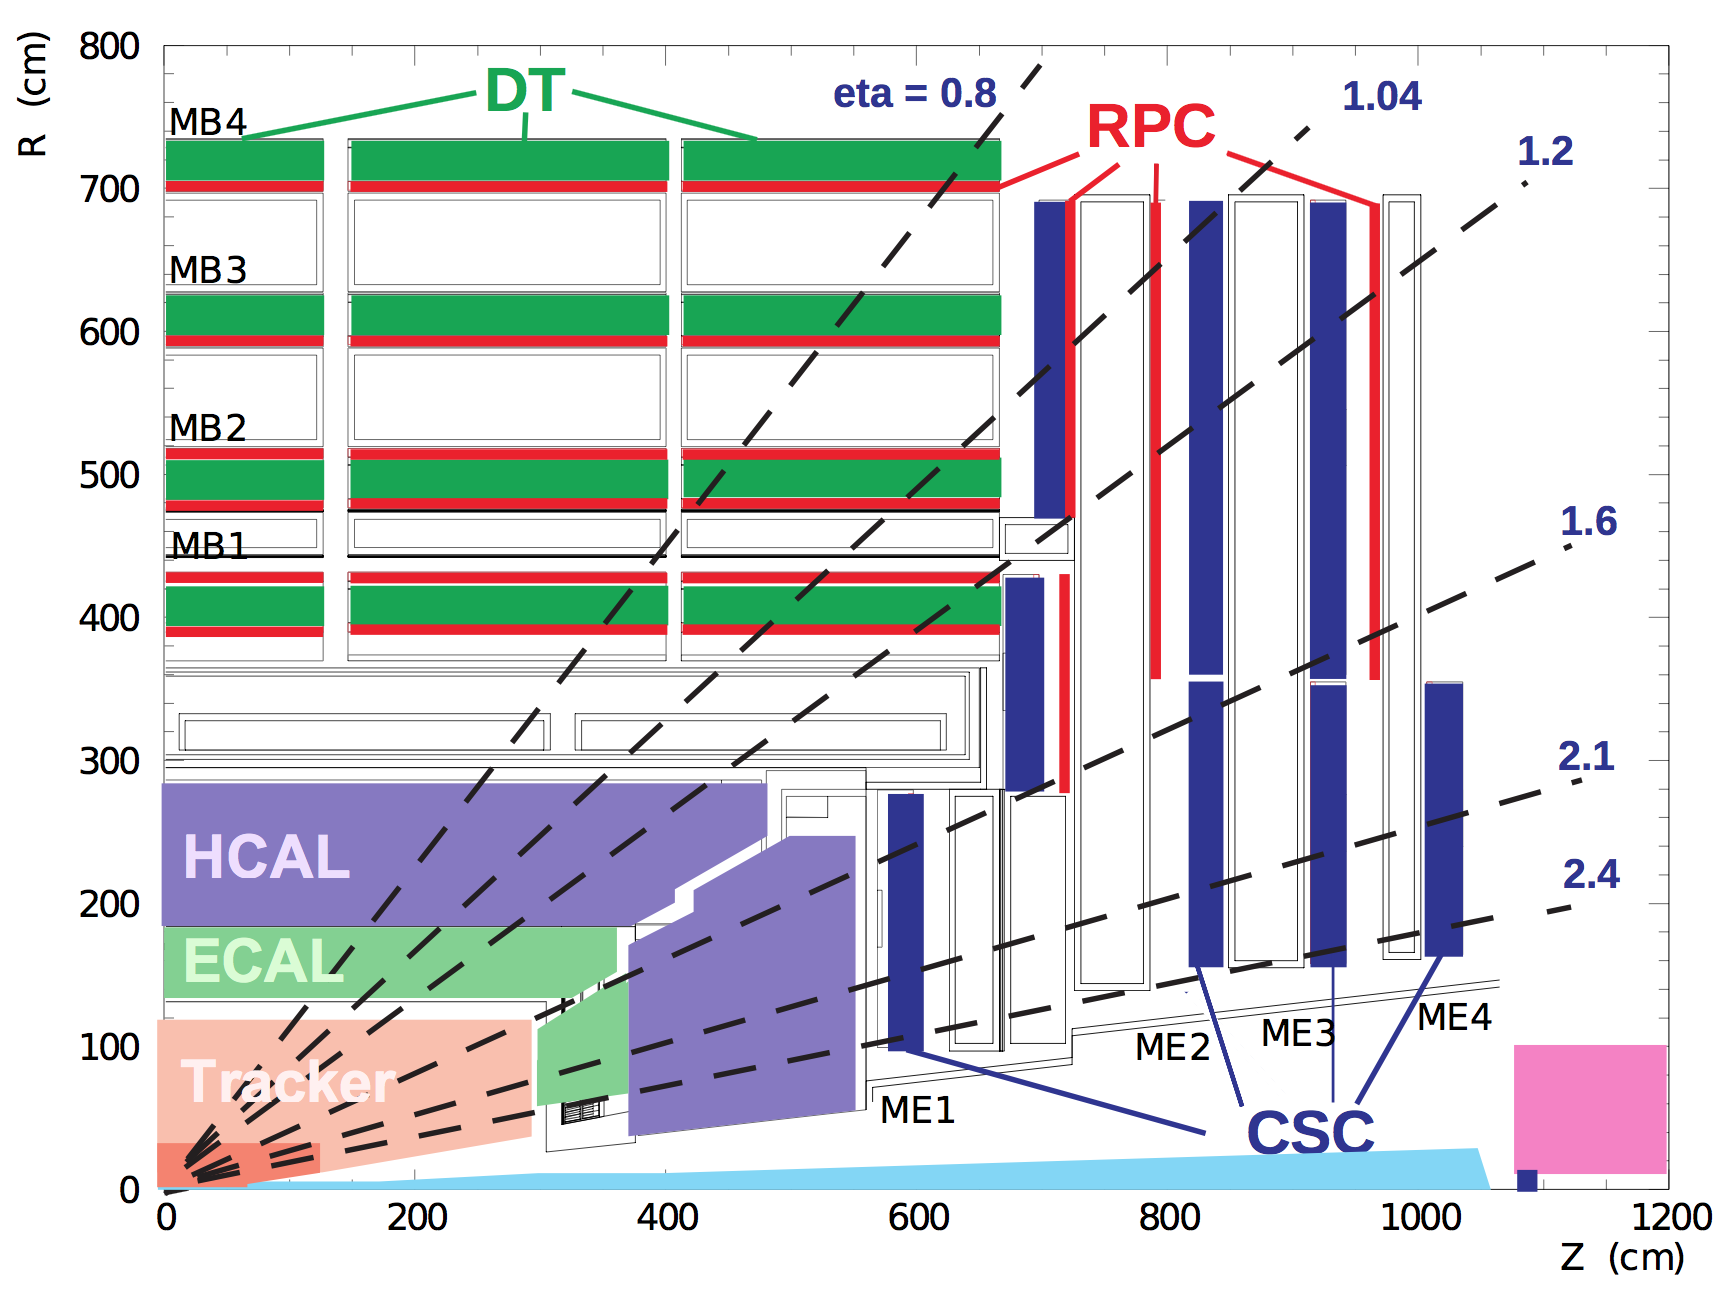
\includegraphics[width=1.0\textwidth]{detectorFigures/cmsMuonSystem.png}
\caption{Schematic \crosssection of one quadrant of the CMS muon detector, showing the arrangement of the various components of the sub-detector: The DTs in the barrel, and CSCs in the endcaps and the RPCs in both. \cite{MuonReco}.}
\label{fig:muonssystem}
\end{figure}

 In the barrel section, the muon system is composed of four concentric layers of \DTs, which are wire chambers filled with a mixture of gaseous Ar and CO$_{2}$. Each DT station consists of twelve layers of wire chambers, with some having their wire oriented parallel to the beam axis and other perpendicular to it. This means that each DT is able to provide a position measurement in both the transverse and longitudinal planes, with 100\um resolution in each. The \DTs have coverage up to $|\eta|<1.3$. 

In the endcaps, the field is less uniform and the neutron fluences become much larger. The muon rate is also much higher than in the barrel. Therefore, a detection system with a faster response and more resistance to radiation is needed. The \CSCs, which are multi-wire chambers comprised of 6 anode wire planes interleaved among 7 cathode panels, satisfy this requirement. They are filled with a mixture of Ar, CO$_{2}$ and CF$_{4}$ gasses, and each station is also able to provide a measurement in both the longitudinal and transverse planes, with a spatial resolution around 85\um. There are four layers of \CSCs in each endcap, with coverage of $0.9<|\eta|<2.4$.

The final detector in the muon system is the array of \RPCs. These are double-gap chambers, and have a fast response with good timing resolution but worse position resolution than the \DTs or \CSCs. The \RPCs are used as a trigger, and can also be used to resolve ambiguities in tracking when there are multiple hits in a chamber. The \RPCs are installed in both the barrel and endcap sections, up to $|\eta|<1.6$~\cite{CMSatLHC,cmsMuon}. 

The transverse energy resolution for muons with \pT below 100\GeV is 1-6\% depending on their position within the detector~\cite{MuonReco}.

\subsection{Trigger and data processing}
\label{sec:cms:trigger}

During operation, bunch crossings occur at a rate of up to 40\MHz. Each instance where the data from a bunch crossing are saved by the detector is known as an event. The storage space taken up by an event is of the order of 1\MB. If \CMS were to keep all the information from each crossing, it would therefore need to save 40\TB of data per second, which is (at the time of writing) entirely impossible to store. Furthermore, the \CMS sub-detector electronics are designed to read out information at a rate of at most 100\kHz, so it is not possible to read out all the collision data either. Therefore, a vast reduction in the number of events selected to be saved is required. In reality, the vast majority of collisions are of no physics interest: many will be low-energy interactions of protons instead of head-on collisions, or will come from well-understood \SM processes. The strategy to reduce the number of selected events is to filter out the commonplace events and save only those which are of physics interest. This is achieved through the \CMS triggering system. The trigger is used to reduce the number of saved events by a factor of order $10^5$. This is achieved through two trigger levels: the \LI and the \HLT.

The \LI consists of programmable, custom-designed electronics. The \LI must reduce the number of output events by a factor of at least 400, since the maximum design bandwidth of the \subdetector electronics readout is 100\kHz. As collisions occur in the \CMS detector, each event is stored in a buffer. A very limited time, 3.2\us, is allocated to decide whether or not to save an event at the \LI. This must include the time taken to transmit the data from the sub-detectors to the \LI and return the decision to accept or not. The 3.2\us latency means that the buffer must be able to hold at least 128 bunch crossings. Due to bandwidth limitations and the short latency, decisions at the \LI are made based on very coarse data from the different detector subsystems individually. There no time to transmit or exploit their full granularity and resolution, or to use detailed correlations between different sub-detectors. The short amount of processing time available also prohibits the use of information from the tracker. Based on the coarse information available, the \LI runs a series of algorithms designed to identify events where processes of interest occur. In the case of a \LI accept, the full event data are transfered off the detector and passed to the \HLT~\cite{CMSatLHC}.

The \HLT consists of a farm of about 1000 commercially-available processors, which run basic reconstruction software and use the output to make a decision on which events to keep. The \HLT provides a further reduction the amount of data stored, decreasing it by a factor of about 100, down to an output of around 400\Hz. This is achieved using simplified versions of the full \CMS reconstruction software, with the full granularity of the information from the \CMS sub-detectors available, including from the tracker~\cite{CMSatLHC}.

Events passing the \HLT are then saved to disk and reconstructed using the full \CMS software for use in physics analyses.


  \chapter{Event reconstruction and selection}
\label{chap:reconstruction}


\section{Introduction}
\label{reco:sec:intro}

This chapter deals with the way in which the simulation and the data collected at the \CMS experiment are reconstructed for use in the \Hgg analysis. 
%This procedure, known as \emph{reconstruction}, is performed on an event-by-event level using custom-built software. 
The processing is performed for each event using the \CMSSW package; the final selection of events specific to the \Hgg analysis is performed using a flexible software framework called \FLASHgg. %The \CMSSW software uses the \PF algorithm, in which energy deposits from the various sub-detectors are combined to reconstruct individual particles. This algorithm is described in \Sec~\ref{reco:sec:pf}. The reconstruction and identification of particles often uses \MVA techniques, known as \BDT\s, which are described in \Sec~\ref{reco:sec:bdt}. 

The \CMS global event description~\cite{CMS-PAS-PFT-09-001,CMS-PAS-PFT-10-001}, referred to as the \PF algorithm, combines information from all \CMS \subdetector\s to reconstruct and identify individual particles. The inputs to this algorithm are the tracks reconstructed in the tracker and muon system, and the clusters of energy reconstructed in the \ECAL and \HCAL. The outputs of the algorithm are objects corresponding to semi-stable particles (photons, electrons, muons, charged hadrons or neutral hadrons). These so-called \PF \emph{candidates} can then be used to reconstruct jets and identify missing energy in the event. The resolution with which momenta of particles can be measured is typically improved using \PF since information from several \subdetector\s is available. In this scheme, \ECAL \SC\s which are not on the extrapolated trajectory of tracks from either the muon system or the tracker are identified as photon candidates. If a track in the tracker is associated to one or more \ECAL \SC\s, then it can be identified as an electron candidate. If a track in the tracker is consistent with a track or multiple hits in the muon system, then it is identified as a muon candidate. Tracks in the tracker which are not associated with any track in the muon system or any deposit in the \ECAL are interpreted as charged hadron candidates. Finally, deposits in the \HCAL which are not associated with any tracks can be identified as neutral hadron candidates.

The same reconstruction algorithms are applied both to the data collected at the \CMS experiment and to simulated samples. % where the interaction of generated particles with the \CMS sub-detectors is simulated. The way in which both data and simulation are obtained are described in \Sec~\ref{th:sec:samples}.
%The way in which both types of sample is obtained 
The data samples and production of simulated samples of \MC events are discussed in \Sec~\ref{reco:sec:samples}.


%The work presented in this thesis involves the study of the Higgs boson decaying to photons, \Hgg. 
It has already been noted in \Sec~\ref{th:sec:higgs_decays} that \Hgg is one of the most sensitive decays with which to study the Higgs boson in the \LHC environment. This is despite it having a small branching fraction (around $0.2\%$) and an irreducible background of \SM processes which produce two photons. The channel benefits from a fully reconstructible final state, which is manifested as a resonant Higgs boson peak on top of a continuous diphoton invariant mass spectrum.
The invariant mass of the diphoton system (\mgg) is given by:
\begin{equation}
\label{reco:eq:mgg}
 \mgg = \sqrt{2 E_{\gamma_{1}} E_{\gamma_{2}} (1-\cos\alpha)}, 
\end{equation}

where $E_{\gamma_{1}},E_{\gamma_{2}}$ represent the energies of the two photons and $\alpha$ represents the opening angle between them. 
The opening angle depends on the directions of the photons. Since the \CMS \ECAL does not provide a directional measurement, the calculation of the opening angle relies on the spatial locations of the photons and of the Higgs boson decay vertex. The \CMS \ECAL can measure the spatial location of the photons with a sufficient resolution that its contribution to the uncertainty on the photon direction is negligible. However, the fact that the photon is a neutral particle and the presence of multiple interaction vertices in the event can lead to the misassignment of the vertex associated with the Higgs boson decay. This produces a large enough uncertainty in the photon direction to significantly worsen the uncertainty on the mass.
Therefore, \Eq~\ref{reco:eq:mgg} indicates that to study \Hgg, the most important steps are measuring the positions and energies of the photons, and locating the Higgs boson \PV. These steps are discussed in \Sec~\ref{reco:sec:photons} and \Sec~\ref{reco:sec:vertex} respectively. 

The main Higgs bosons production processes or \emph{modes} are described in \Sec~\ref{sec:th:higgs_production_modes}. At leading order, in the dominant production mode (\ggH), the final state consists only of the two Higgs decay photons. However, for other production modes, the Higgs boson can be produced in association with other particles. These additional particles can be reconstructed, providing information on the mode by which the Higgs boson is produced. The methods used to reconstruct such particles are described in \Sec~\ref{reco:sec:other}.

%\section{Common reconstruction methods}
%\label{reco:sec:tools}

%Some analysis methods occur repeatedly throughout the reconstruction process. A short description of these techniques is given here.

%\subsection{The particle-flow algorithm}
%\label{reco:sec:pf}



%\subsection{Tag-and-probe}
%\label{reco:sec:tagandprobe}


\section{Samples}
\label{reco:sec:samples}
\subsection{Simulation samples}

Samples of simulated signal events are produced for each of the main Higgs boson production modes for a range of values of \mH between 120 and 130\GeV. The \crosssection and branching fractions used for the simulations under each \mH hypothesis are those recommended by the \LHCHXSWG~\cite{LHCHXSWGYR4}. Signal samples are used to: prepare classifiers, for instance using the \BDT method (see \Sec~\ref{reco:sec:bdt}); validate reconstruction and selection algorithms; and produce signal models (see \Sec~\ref{model:sec:signal_model}). Signal simulations are produced at parton-level using the generator \Madgraph~\cite{Madgraph}, which makes use of perturbative \QCD at \NLO. The parton-level samples are then interfaced with \Pythia~\cite{Pythia8}, using the tune \PythiaTune~\cite{PythiaTune}, which models the subsequent showering and hadronisation of partons. 

Samples of simulated events are also generated for each of the main backgrounds of the \Hgg decay. Background samples are used to: train \BDT\s; validate reconstruction and selection algorithms; and optimise the categorisation scheme. The irreducible background is composed of \SM processes which yield two genuine photons from a \pp interaction in the final state, and are modelled using the \Sherpa~\cite{Sherpa} generator. The reducible background represent events where some jets are incorrectly identified as isolated photons. The largest contributors to the reducible background are \gammaJet and \QCDmultijet events, which are modelled using the \Pythia generator, where a filter designed to enhance the fraction of events with a large component of electromagnetic energy is applied. %The filter required a potential photon signal (photon, electron, or neutral hadrons, with $pt>15 \GeV$
\DY, \Wg and \Zg samples are also used for validation purposes, and these are simulated using \Madgraph. 

The simulated samples take into account the effects of the multiple interactions, other than the hard scattering interaction, taking place in each bunch crossing. These additional interactions are collectively referred to as \PU. The effect of \PU in previous and subsequent bunch crossings is also modelled. The samples are reweighted such that their \PU distributions match the data before they are used in the analysis.
For all simulated samples, the detailed response of the \CMS detector is modelled using \Geant~\cite{Geant}.


\subsection{Data samples and trigger} % including triggers
\label{sec:reco:data}

The data sample analysed in this thesis was recorded using the \CMS detector in between March and \finaldatatakingmonth 2016, during \pp LHC collisions at $\sqrt{s}=13\TeV$. It corresponds to an integrated luminosity of \thisanalysislumi\ifb. As described in \Sec~\ref{sec:cms:trigger}, events recorded for analysis at \CMS must pass the requirements of the two \CMS triggering systems: the \LI and the \HLT. 

The \LI requires either a deposit in the \ECAL with $\pT>25\GeV$ or two deposits with $\pT>15\GeV$ and $\pT>10\GeV$ respectively. Events passing the \LI are processed at the \HLT, where a basic clustering is applied to the candidate photon deposits. The requirements for an event to be saved to the double-photon sample by the \HLT are as follows:

%such as the invariant mass of diphoton pairs (\mgg), the transverse energy of candidate photons \ET and the \RNINE of a candidate, For an event to be saved in the double-photon sample, the trigger requires:
\begin{itemize}
\item the event contains two candidate photons, with $\mgg > 90\GeV$;
\item the candidate photon with most energy satisfies $\ET >30\GeV$; 
\item the candidate photon with second-most energy satisfies $\ET >18\GeV$;
%\item the two candidate photons must either have a large value of \RNINE (defined as the sum of the energy of the $3\times3$ array of crystals around the most energetic crystal in a \SC, divided by the energy of the \SC) or pass a loose calorimeter-based identification and isolation requirement.
\item both candidate photons pass a basic calorimeter-based identification using shower shape and isolation requirements.
\end{itemize}


Events passing the \LI and \HLT requirements are saved for further processing. The efficiency of the trigger for signal events passing the preselection requirements described in~\Sec~\ref{reco:sec:pho:preselection} is studied using the \TagAndProbe method~\cite{TagAndProbe}. This is a common way to determine the efficiency of a selection $S$ in data, and is used at several stages in this analysis. The technique exploits resonances decaying to pairs of particles, in this case \Zee. The events used for the \TagAndProbe method are selected such that the invariant mass of the decay products are near the mass peak of the resonant particle, thus ensuring high-purity sample. A strict identification requirement is imposed on one of the decay products, referred to as the \emph{tag}, and while a very loose identification requirement is imposed for the other decay product, referred to as the \emph{probe}. The requirements applied to the probe should be loose enough that they do not affect the efficiency of $S$. The efficiency of $S$ is then the fraction of probes which satisfy $S$. 
The \LI efficiency is found to be above 97.5\% in the \EB and above 92\% in the \EE. The efficiency of the \HLT is found to be above 97\% in the \EB and 96\% in the \EE. %The \Zee data sample is obtained using a special trigger which relies on loose requirements on a single electron. Using an additional selection on the invariant mass of events with two electrons, it is possible to select a high-purity \Zee sample using this trigger. The electrons are reconstructed as photons and passed through the reconstruction steps detailed in this chapter. 


\section{Photon reconstruction} 
\label{reco:sec:photons}



\subsection{Clustering of ECAL deposits}

%The most important \subdetector for the reconstruction of photons is the \ECAL. 
About 95\% of the energy of a single electromagnetic shower in the \ECAL is contained in a $5\times5$ array of crystals. However, particles can have several showers associated with them. Photons travelling towards the \ECAL may undergo pair conversion ($\gamma \rightarrow \Pep \Pem$) in the detector material, resulting in two nearby or overlapping showers usually separated in $\phi$. Electrons or positrons are deflected by the magnetic field, and radiate photons from bremsstrahlung, resulting in multiple showers spread out in the $\phi$-direction. 

%A \emph{clustering} algorithm~\cite{CMS-PAS-EGM-13-001,CMS-PAS-EGM-14-001} attempts to build a \SC which associates all the individual energy deposits of a photon coming from the vertex. 
A \emph{clustering} algorithm~\cite{CMS-PAS-EGM-13-001,CMS-PAS-EGM-14-001} groups the \ECAL energy deposits into \SC\s. Each \SC is designed to associate all the individual deposits resulting from a photon or electron originating at a primary interaction vertex.
The algorithm begins by identifying \emph{seed} crystals as those with the largest amount of energy in the local area, above a predefined minimum noise threshold. The threshold %is between 80\MeV and 300\MeV depending on the pseudorapidity region, and 
represents approximately two standard deviations of the electronic noise in the \ECAL. Next, clusters are obtained by iteratively grouping crystals which have a common side with a crystal already in the cluster if their energy is above another predefined threshold. The location of a cluster is defined as the logarithmic energy-weighted average position of the individual crystals which compose it. During the iterative clustering process, if a crystal could belong to different clusters, its energy is shared between them according to the distance between the crystal and each cluster, assuming a Gaussian shower profile. Finally, additional clusters can be merged with the original cluster to form a \SC if they are aligned in the $\eta$-direction and lie within an extended window in the $\phi$-direction. This final step is designed to recover deposits resulting from bremsstrahlung.
%\phifrom the are merged into \SC\s by gathering those which lie between two parabolas extending into the $\phi$-direction as a function of $\eta$. %This gives the \SC\s a mustache-like shape, designed to recover the energy of bremsstrahlung photons and to mitigate the effect of \PU.
%The \SC\s obtained from clustering the \ECAL deposits are fed into the \PF algorithm described in \Sec~\ref{reco:sec:pf}, and are interpreted as either electron or photon candidates. 
The clusters and \SC\s are fed into the \PF system, and are used to build electron and photon candidates.

\subsection{Common variables used for photon and electron studies}
\label{sec:reco:photon:showershapes}

A number of variables are used to characterise the development of the electromagnetic shower within the PbWO$_4$ crystals. These variables are used in various stages of the reconstruction and selection, and for convenience some of the most important ones are defined here.
%\underline{General variables}:
%\begin{itemize}
%\item $\rho$, the median energy density in the event;
%\item \emph{Electron veto}, a variable which returns ``false'' if the \PF algorithm determined that a \SC corresponds to an electron.
%\end{itemize}
%

\vbox{\underline{Shower shape variables}:
\begin{itemize}
\item \RNINE, the energy in the $3\times3$ array of crystals around a seed crystal divided by the energy of the \SC. The \RNINE variable gives information about whether a photon converted (low values of \RNINE) or not (high values of \RNINE);
\item $S_{4}$, the energy of the most energetic $2\times2$ array of crystals containing the seed crystal, divided by the energy of the \SC;
\item $n_{\textrm{clusters}}$, the number of clusters in a \SC;
\item $\sigma_{\eta}$, the standard deviation of the logarithmic energy-weighted $\eta$-position of individual crystals within the \SC (or the $5\times5$ array centred around the seed in some cases);
\item $\sigma_{\phi}$, the standard deviation of the logarithmic energy-weighted $\phi$-position of individual crystals within the \SC (or the $5\times5$ array centred around the seed in some cases);
\item $\sigma_{RR}$, the width of the shower in the radial direction (defined in the endcaps only);
\item $cov_{\eta \phi}$, the covariance of the single-crystal values of $\eta$ and $\phi$ for the $5\times5$ array centred around the crystal with the most energy; %what?
\item $E_{\textrm{seed}}/E_{SC}$, $E_{\textrm{seed}}/E_{3\times3}$, $E_{\textrm{seed}}/E_{5\times5}$, ratios of the energy of the seed crystal and energy of: the \SC, the $3\times3$ array centred around the seed, and the $5\times5$ array centred around the seed respectively;
\item \HoE, the ratio of the energy deposited in the \HCAL in a cone of radius $R=0.15$ directly behind a \SC and the energy of that \SC as recorded in the \ECAL. 
\end{itemize}
\underline{Isolation variables}:
\begin{itemize}
\item $Iso^{\textrm{PF}\gamma}_{R=0.3}$, \PF photon isolation i.e.~the sum of the transverse energy of all \PF photons inside a cone of radius $R=0.3$ around the candidate photon, where the energies have been corrected according to the median energy density in the event ($\rho$);
\item $Iso^{\textrm{PF ch. had.}}_{R=0.3}(V)$, \PF charged hadron isolation i.e.~the sum of the transverse energy of all \PF charged hadrons associated with a particular vertex $V$ inside a cone of radius $R=0.3$ around the candidate photon. This quantity is typically calculated with respect to the selected primary vertex, and also for the vertex which has the largest isolation sum (referred to as the \emph{worst vertex}). The latter helps to reject photons candidates which are misidentified jets originating from pileup;
\item $Iso^{\textrm{tracker}}_{0.04<R<0.30}$ tracker hollow cone isolation, i.e.~the sum of the \pT of all tracks inside a hollow cone of radius $0.04 < R < 0.30$ around the photon candidate. 
\end{itemize}}

\subsection{Photon preselection}
 \label{reco:sec:pho:preselection}

The photon candidates considered in the \Hgg analysis are required to satisfy certain requirements on their kinematics, shower shapes and isolation. All photon candidates are required to pass an \emph{electron veto}, which requires that there be no track with a hit in the inner layer of the pixel detector (not matched to a reconstructed photon conversion vertex) pointing to the \SC~\cite{CMS-PAS-EGM-14-001}. Photons candidates are then grouped into \emph{diphotons} by determining all possible pairs of photons in the event. For each diphoton, the photon with the largest \pT (the \emph{leading} photon) must satisfy $\pT>30\GeV$ while the photon with the second-largest \pT (the \emph{subleading} photon) must satisfy $\pT>20\GeV$. Additional requirements are made on a per-photon basis on the following variables: $\sigma_{\eta}$, \HoE, $Iso^{\textrm{PF}\gamma}_{R=0.3}$, $Iso^{\textrm{PF ch. had.}}_{R=0.3}$, $Iso^{\textrm{tracker}}_{0.04<R<0.30}$ and \RNINE. 

Since no triggers are defined in the simulation, the preselection is designed to be more stringent than the triggering requirement described in \Sec~\ref{sec:reco:data}. This ensures that trigger efficiency after the preselection is close to $1$.

The preselection efficiency, for all requirements aside from the electron veto, is measured in data and simulation using \Zee events, using a \TagAndProbe technique for photons in different regions of $\eta$ and \RNINE. The results can be seen in \Table~\ref{tab:reco:preslection_eff}. The efficiency of the electron veto is measured separately using a sample of \Zmmg events, and found to be between 96\% and 100\%.

\begin{table}[htbp]
\begin{small}
\begin{center}
\resizebox{\textwidth}{!}{
\begin{tabular}{|l|c|c|c|c|c|c|c|}
\hline
& \multicolumn{ 3}{c|}{DATA} & \multicolumn{2}{c|}{Simulation} & \multicolumn{ 2}{c|}{Ratio} \\
\hline
& Eff. & Stat. Unc. & Syst. Unc. & Eff. & Stat. Unc. & Eff. & Unc. \\
%\hline
% & \multicolumn{7}{c|}{}\\
\hline
ECAL Barrel; $\RNINE>$0.85 & 0.9451 & 0.0006 & 0.0192 & 0.9374 & 0.0007 & 1.0080 & 0.0192 \\
ECAL Barrel; $\RNINE<$0.85 & 0.8255 & 0.0012 & 0.0119 & 0.8258 & 0.0009 & 0.9960 & 0.0120 \\
ECAL Endcap; $\RNINE>$0.90 & 0.9099 & 0.0008 & 0.0212 & 0.9127 & 0.0010 & 0.9969 & 0.0212 \\
ECAL Endcap; $\RNINE<$0.90 & 0.4993 & 0.0018 & 0.0249 & 0.5024 & 0.0016 & 0.9938 & 0.0250 \\
\hline
\end{tabular}
}
\end{center} 
\end{small}
\caption{Photon preselection efficiency (using all requirements aside from the electron veto) measured using \Zee
events in data and simulation with a \TagAndProbe technique.}
\label{tab:reco:preslection_eff}
\end{table}


\subsection{Boosted decision trees}
\label{reco:sec:bdt}

The reconstruction of photons and other particles uses \MVA techniques at several stages in the form of \BDT\s~\cite{friedman2009}. A \BDT is obtained using the \DT method, where an additional technique known as \emph{boosting} is applied. Problems where a \BDT is of use always involve a list of items with $N_{\textrm{inputs}}$ \emph{features} or \emph{input variables}, labelled here $\vec{x} =(x_1, ... ,x_{N_{\textrm{inputs}}})$, and a property $y$, the \emph{target variable} to be determined. The objective of a \BDT is to produce a function $F(\vec{x})$ which is an estimate of the true value of $y$ for a given set of input variable values~\cite{friedman2001}. 
%There are two common uses for \BDT\s: \emph{classification} and \emph{regression}. 

The most common application for \BDT\s is event classification, for instance to determine whether a photon candidate was produced during a hard scatter or not: the target variable takes discrete values (background or signal). In other cases, \BDT\s are used for regression problems, where the target variable is continuous rather than discrete. For example, the energy correction for \SC\s in the \ECAL ($F_{\text{SC}}$ in \Eq~\ref{eq:cms:ecal:energy}) is obtained using a regression \BDT, as is described in \Sec~\ref{sec:reco:photon:phoenergybdt}. The \BDT\s used in this thesis are produced using the \TMVA framework~\cite{TMVA} as part of the \ROOT~\cite{root} software package. 

In general, a \BDT is a linear combination of \DT\s~\cite{friedman2009}. A \DT is obtained using a \emph{training dataset} consisting of a list of items $(\vec{x}_{m},y_{m},w_{m})$ for $m=1,...,N_{\textrm{items}}$, where $\vec{x}_{m}$ is a set of input variables values, $y_{m}$ is the true value of the target variable and items can be weighted with weight $w_{m}$. In the simplest case, the value of $y_{m}$ is binary: signal or background. A numerical value, $1$ and $-1$ say, can be assigned to these two options respectively. The following description uses this binary output example, but can be generalised for $y_{m}$ to take any number of discrete values for classification \DT\s, or continuous values in the case of regression \DT\s.
To construct a \DT, the training dataset is first split into two subsamples by applying a selection, which will be referred to as a \emph{cut}, on one or more of the input variables. The \emph{purity} $p(s)$ of a subsample $s$ is the proportion of signal items, given by:

\begin{equation}
 p(s) = \frac{\sum_{m=1}^{N_{\textrm{items}}^{s}} w_{m} \cdot \textrm{Bool}(y_m=1)}{\sum_{m=1}^{N_{\textrm{items}}^{s}} w_{m}}, 
\end{equation}

where $N_{\textrm{items}}^{s}$ is the number of items in the subsample and $\textrm{Bool}(X)$ is equal to $1$ $(0)$ if $X$ it true (false). 
The cuts on the input variables are chosen to maximise the separation of signal and background in the resulting subsamples. This is achieved by minimizing a separation criterion. 
A common separation criterion is the \emph{Gini index} $2p(s)(1-p(s))$, which has a maximum at $0.5$ for subsamples with an equal amount of signal and background items and gives $0$ in cases where all items are of the same type (signal or background). Many other separation criteria exist, for instance \emph{cross-entropy, misclassification error, statistical significance} and \emph{average squared error}.
Each subsample can then be further split by a new set of cuts on the input variables. This procedure is repeated iteratively for each subsample until either the number of iterations reaches some predefined threshold known as the \emph{tree depth}, or if the subsample satisfies some predetermined requirement on the value of the separation criterion. Each subsample obtained after the final set of cuts has been applied is known as a \emph{leaf}. The output score of the items in a given leaf is then $1 $ if $p(s)>0.5$ and $-1$ if $p(s)\leq0.5$.

The procedure known as boosting~\cite{friedman2001} helps to improve the performance of a \DT, for example by reducing the risk of overfitting the \DT to statistical fluctuations in the training sample. Many boosting algorithms exist, but in all cases several individual \DT\s are produced, each trained on subsets or modified versions of the training dataset. The final \BDT is a linear combination of the individual \DT\s. Supposing that there are $N_{\textrm{DT}}$ individual \DT\s, labelled as $f_{l}(\vec{x},\vec{\alpha}_{l})$ where $l=1,..,N_{\textrm{DT}}$ and $\vec{\alpha}_{l}$ is the set of cuts in the corresponding \DT, the full \BDT, $F$, is written as:

\begin{equation}
\label{reco:eq:bdt}
F(\vec{x},\vec{\beta},\vec{\alpha}) = \sum_{l=1}^{N_{\textrm{DT}}} \beta_{l} f_{l}(\vec{x},\vec{\alpha_{l}}), 
\end{equation}

where $\vec{\beta}=(\beta_{1},...,\beta_{N_{\textrm{DT}}})$ is the set of coefficients applied to each \DT in the \BDT. The values of of $\vec{\beta}$ are determined by the boosting algorithm~\cite{friedman2009,TMVA}. A consequence of \Eq~\ref{reco:eq:bdt} is that the output of the \BDT is no longer a discrete value of $\pm1$, but instead a semicontinuous variable between $-1$ and $1$. 

%The simplest and most common boosting algorithm is \emph{adaptive boosting}. In adaptive boosting, the first \DT is trained on the full training dataset as usual. The training dataset is then reweighted so that items which were assigned an incorrect output score by the previous \DT (the so-called \emph{weak learners}) are given a larger weight and the items which were correctly classified are given a smaller weight. The next \DT is then trained on the modified dataset, and the whole procedure is repeated over a large number of iterations. The final $\vec{\beta}$ for adaptive boosting algorithms is given by the logarithm of the weights applied to the dataset at each step. A more robust method is \emph{gradient boosting}, where the values of the individual components of $\vec{\alpha}$ and $\vec{\beta}$ are varied in such a way as to minimise the \emph{loss function} $L(F,y)$, which is a measure of the deviation of the \BDT output score from the true value of $y$ across all items in the training dataset. Popular choices for the loss function include $L(F,y) = ( y - F(\vec{x},\vec{\beta},\vec{\alpha}))^2$ and$L(F,y) = \ln (1 + e^{-2F(\vec{x},\vec{\beta},\vec{\alpha})y})$~\cite{friedman2009,TMVA}.



\subsection{Photon energy reconstruction BDT}
\label{sec:reco:photon:phoenergybdt}

The energy of a \SC is given by \Eq~\ref{eq:cms:ecal:energy}, %The \ECAL response is equalised using a per-crystal set of inter-calibration constants. A time-dependent correction for the transparency of the crystals is applied, and the global scale which converts the pulse amplitudes to energy measurements is set during the calibration process. 
where $F_{\text{SC}}$ is a correction to the \SC energy which takes into account second order effects such as how well a \SC is contained within a crystal. This correction is obtained using a per-\SC regression \BDT, referred to here as \PhoEnergyBdt, assuming that the \SC corresponded to a photon deposit. %A similar but separate \BDT is used to correct the energy of the \SC under the assumption that the energy was deposited by an electron.

The target variable for the \PhoEnergyBdt is the ratio of the true photon energy $E_{true}$ and the raw energy of the \SC $E_{SC}$. The \PhoEnergyBdt is trained separately for \SC\s in the barrel and endcaps, using a simulated sample of double-photon events reweighted to flatten the \pT and $\eta$ distributions of the individual photons. The set of input variables is listed below:
\begin{itemize}
\item Shower shape variables, such as those defined in \Sec~\ref{sec:reco:photon:showershapes}, which provide information about whether a photon converted, the extent to which it began showering before hitting the \ECAL, and the extent to which the shower was contained within the \ECAL;
\item Position variables, i.e.~the position of the seed crystal in terms of crystal indices $i\eta$ and $i\phi$, the distance between the positions of the \SC and the seed crystal and the distance between the seed crystal and the boundaries between \ECAL modules. These variables provide information about energy lost through gaps in between the detector modules and between crystals; 
% ieta, iphi, 
\item Noise variables, i.e.~variables related to \PU such as the number of reconstructed vertices in the event and the median energy density in the \ECAL as a function of position.
\end{itemize}

The training is done using a \emph{semiparametric likelihood} technique. In this technique, the distribution of the target variable from the training sample is fitted to a functional form, in this case a \DCB~\cite{CrystalBallFunction}. The \DCB is chosen as it is typically a good fit for processes modelling detector resolutions. It consists of a Gaussian core and power-law tails on each side, with 6 independent parameters: the width $\sigma_{DCB}$ and mean $\mu_{DCB}$ of the core, the left tail cutoff and power parameters $\alpha_{DCB}^{L},n_{DCB}^{L}$ and the right tail cutoff and power parameters $\alpha_{DCB}^{R},n_{DCB}^{R}$. The fitting is performed by minimizing \NLL:

\begin{equation}
\label{reco:eq:regression:dcb}
 - 2\ln \mathcal{L} = -2 \sum_{\textrm{photons}} \ln P_{DCB}( \frac{E_{true}}{E_{SC}} | \mu_{DCB}, \sigma_{DCB}, \alpha_{DCB}^{L},n_{DCB}^{L}, \alpha_{DCB}^{R},n_{DCB}^{R} ) , 
\end{equation}
 where $P_{DCB}$ is the \DCB probability distribution and all the \DCB parameters are functions of $\vec{x}$, the set of input variables for \PhoEnergyBdt. The nonparametric dependence of the \DCB parameters on $\vec{x}$ is obtained using separate \BDT\s, where a new tree is produced for each iteration of the \NLL fit. The most probable value of $E_{true}$ is then given by $\mu_{DCB}(\vec{x}) \times E_{SC}$ and the relative energy resolution for each photon is approximated by $\sigma_{DCB}(\vec{x}) / \mu_{DCB}(\vec{x})$.

The performance of the \PhoEnergyBdt is illustrated using a simulated sample of \Hgg photons where $\mH=125\GeV$ in \Fig~\ref{fig:reco:pho_regression}.

\begin{figure}[hp]
\centering
\subfloat[EB]{
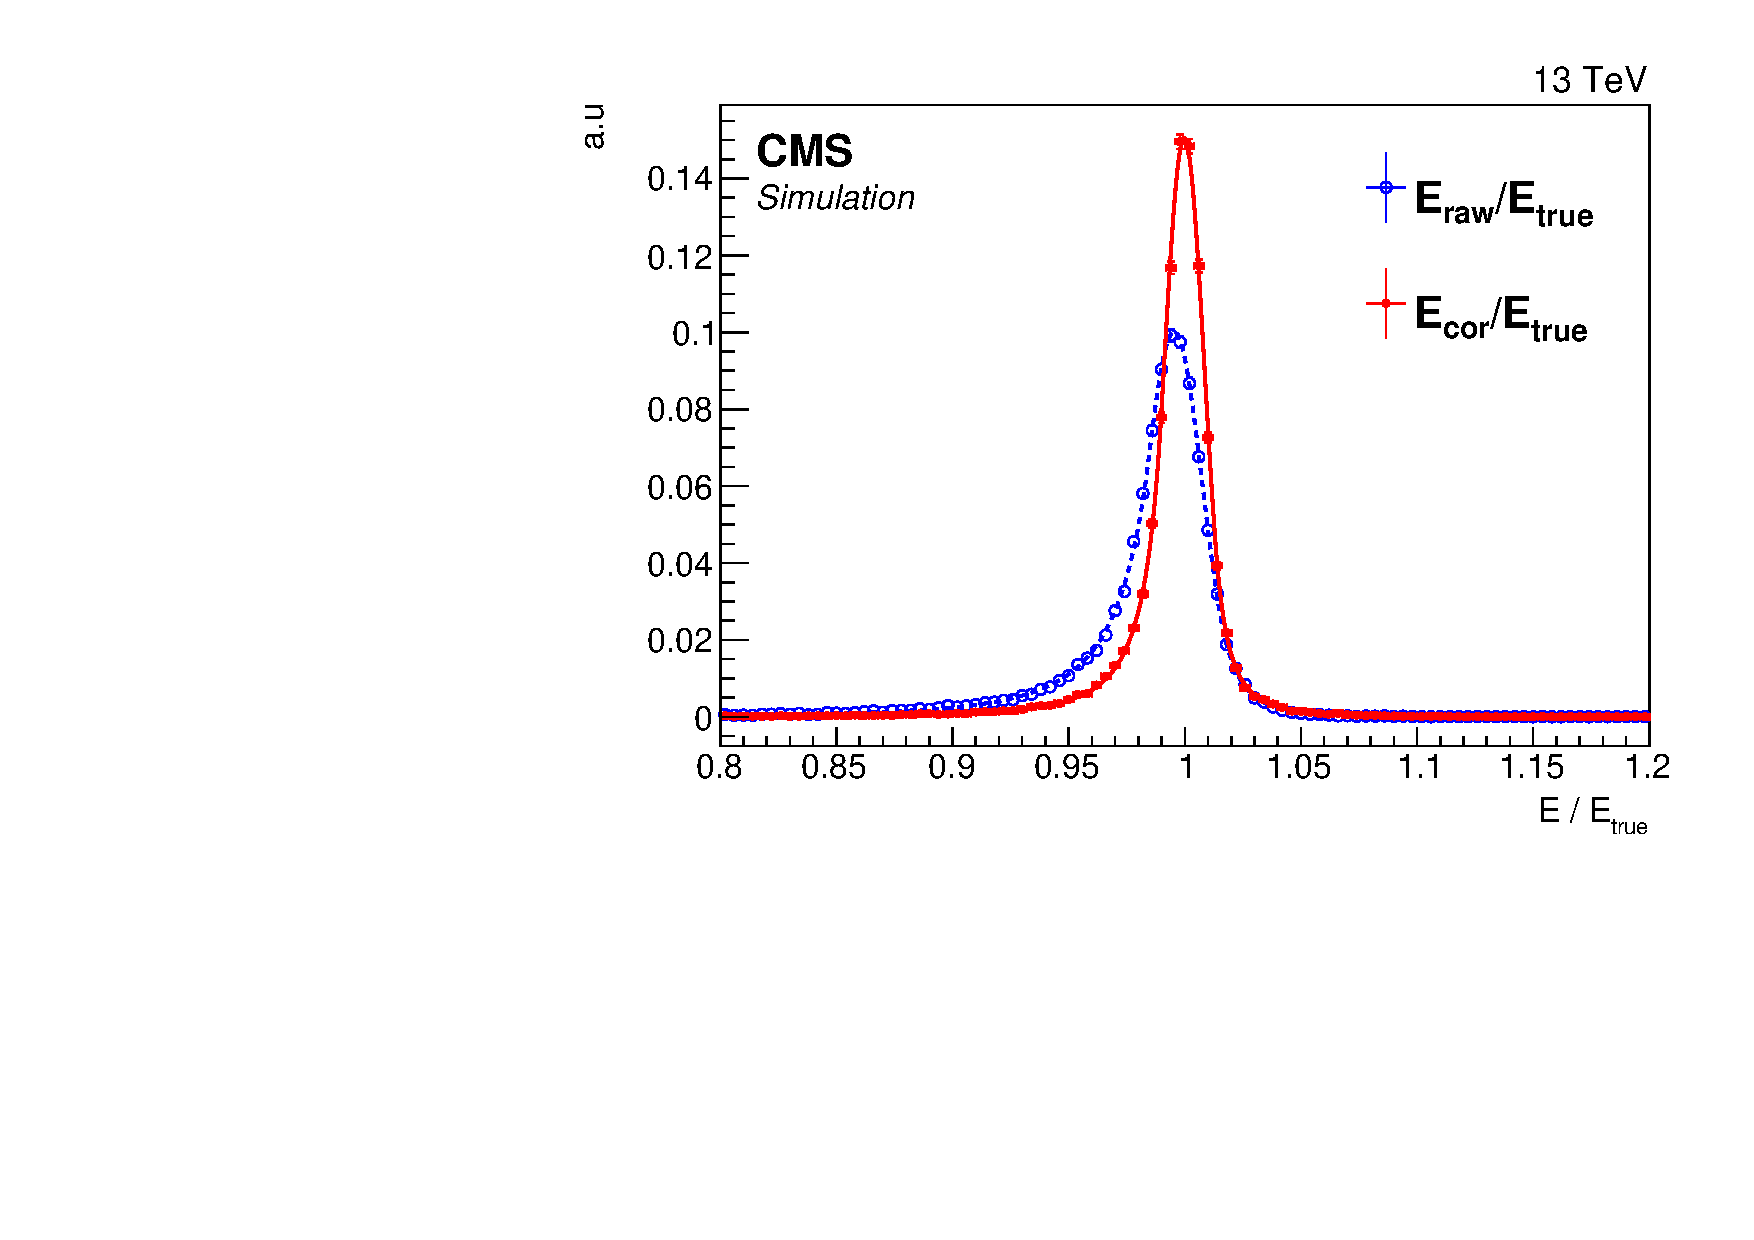
\includegraphics[width=0.6\textwidth]{recoFigures/RegressionEB_Hgg.pdf}
}\\
\subfloat[EE]{
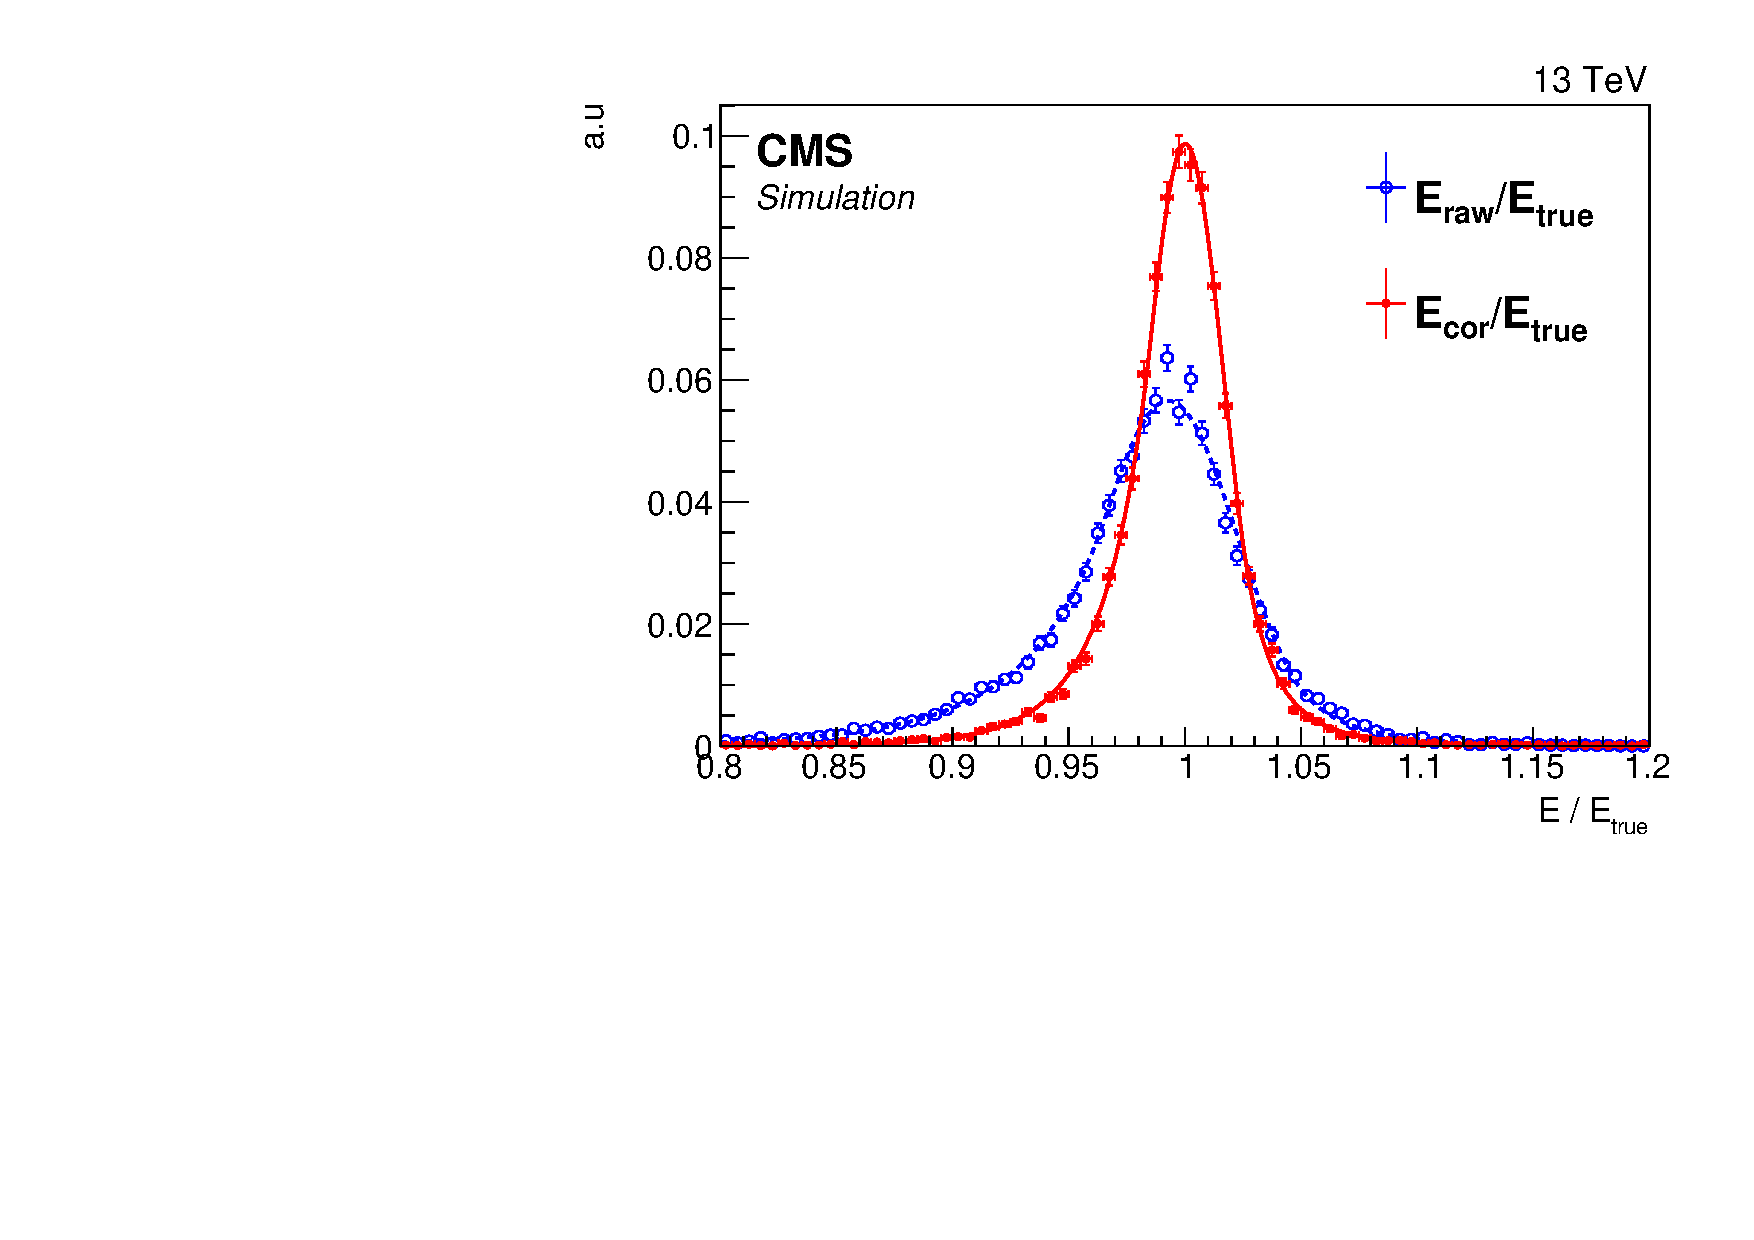
\includegraphics[width=0.6\textwidth]{recoFigures/RegressionEE_Hgg.pdf}
}
\caption{The ratio of the SC energy, shown before the \PhoEnergyBdt correction is applied ($E_{raw}$) and after the correction is applied ($E_{cor}$), and true energy ($E_{true}$) of simulated photons in a sample of \Hgg decays where $\mH=125\GeV$, separately for the EB (a) and the EE (b). All distributions have been fitted to DCB functions.}

\label{fig:reco:pho_regression}
\end{figure}


\subsection{Photon identification BDT}
%In order to separate \emph{prompt} photons (which were produced at the \PV) from \emph{fakes} such as misidentified jets, a per-photon \BDT referred to as \PhoIdBdt is applied 
To reduce the large background originating from the decay of neutral hadrons (predominantly neutral pions) a per-photon \BDT referred to as \PhoIdBdt is applied to photon candidates which pass the preselection described in \Sec~\ref{reco:sec:pho:preselection}. The \PhoIdBdt is trained on a \gammaJet sample where the photon candidates which are geometrically matched to a generator-level photon from a \pp interaction are defined as signal. Photon candidates which have no generator-level photon match, and are therefore likely to have resulted from a misidentified neutral hadron or jet, are defined as the background. In both cases, photon candidates are required to pass the event preselection. To reduce the dependence of the \PhoIdBdt on the kinematics of the photon, the signal photons are reweighted such that their \pT and $\eta$ distributions match those of the background photons. The input variables for the \PhoIdBdt are $\sigma_{\eta}$, $cov_{\eta \phi}$ , $S_{4} $, \RNINE , $\sigma_{\eta} $, $\sigma_{\phi }$, $\sigma_{RR}$, $Iso^{\textrm{PF}\gamma}_{R=0.3}$, $Iso^{\textrm{PF ch. had.}}_{R=0.3}(\textrm{selected vertex})$, $Iso^{\textrm{PF ch. had.}}_{R=0.3}(\textrm{wrong vertex})$, $\rho$, $\eta_{SC}$ and $E_{SC}$. 

A loose requirement on the output of the \PhoIdBdt is applied to all photons considered in the analysis, such that 99\% of the signal photon candidates are kept while a large fraction of background photon candidates are removed. The \PhoIdBdt output score of each photon is then used as a measure of the ``quality'' of each photon, and used as an input for the classification \BDT described in \Sec~\ref{cat:sec:dipho_bdt}.
The \PhoIdBdt is validated by comparing the output score for data and simulation for diphoton events (\Fig~\ref{fig:reco:photon_id_score_hgg_bkg}) and for $\Zee$ events (\Fig~\ref{fig:reco:photon_id_zee_validation}) where the electron veto requirement is inverted. A systematic uncertainty of approximately $3\%$ on the value of the \PhoIdBdt output score is introduced to account for the differences between data and simulation.


\begin{figure}[hptb]
\centering 
%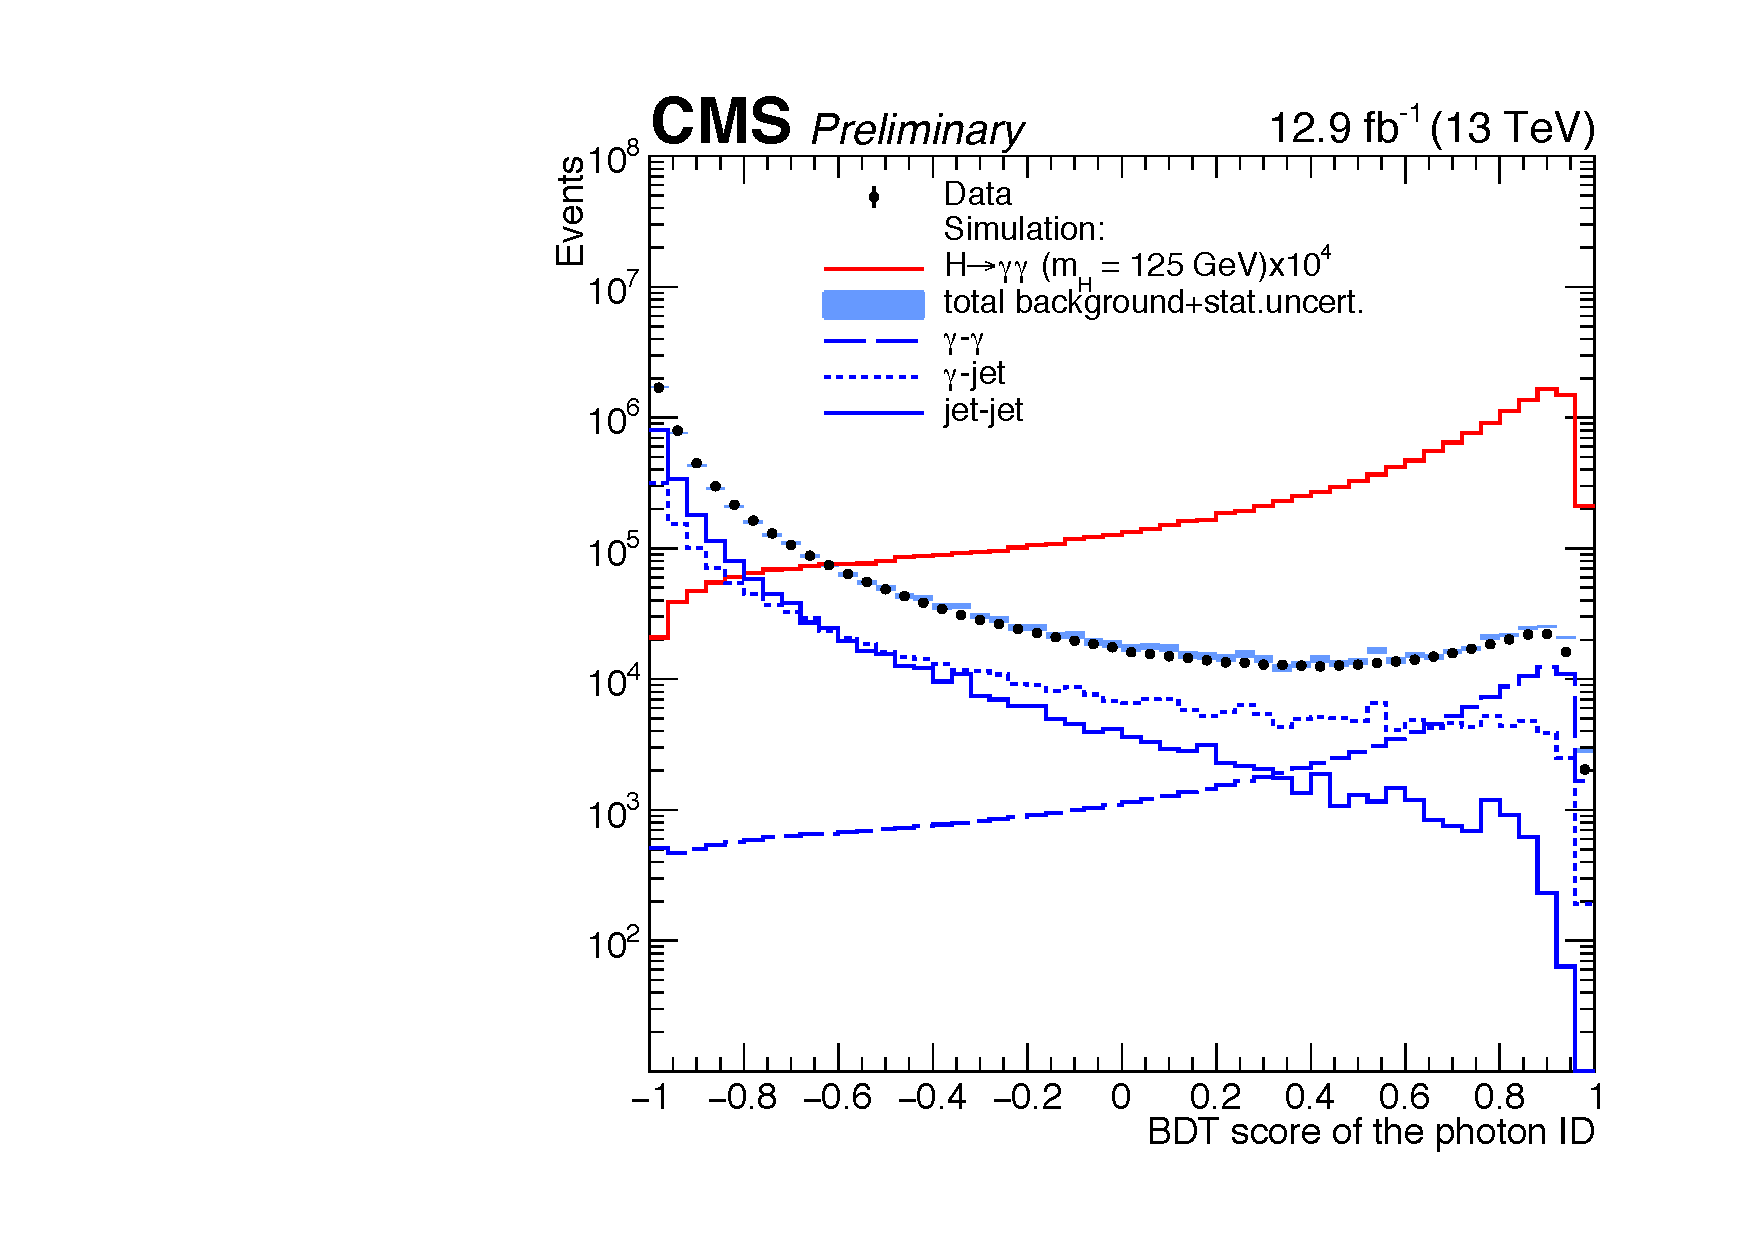
\includegraphics[width=0.47\textwidth]{recoFigures/validation_phoID_ICHEP_4sideTicks.pdf}
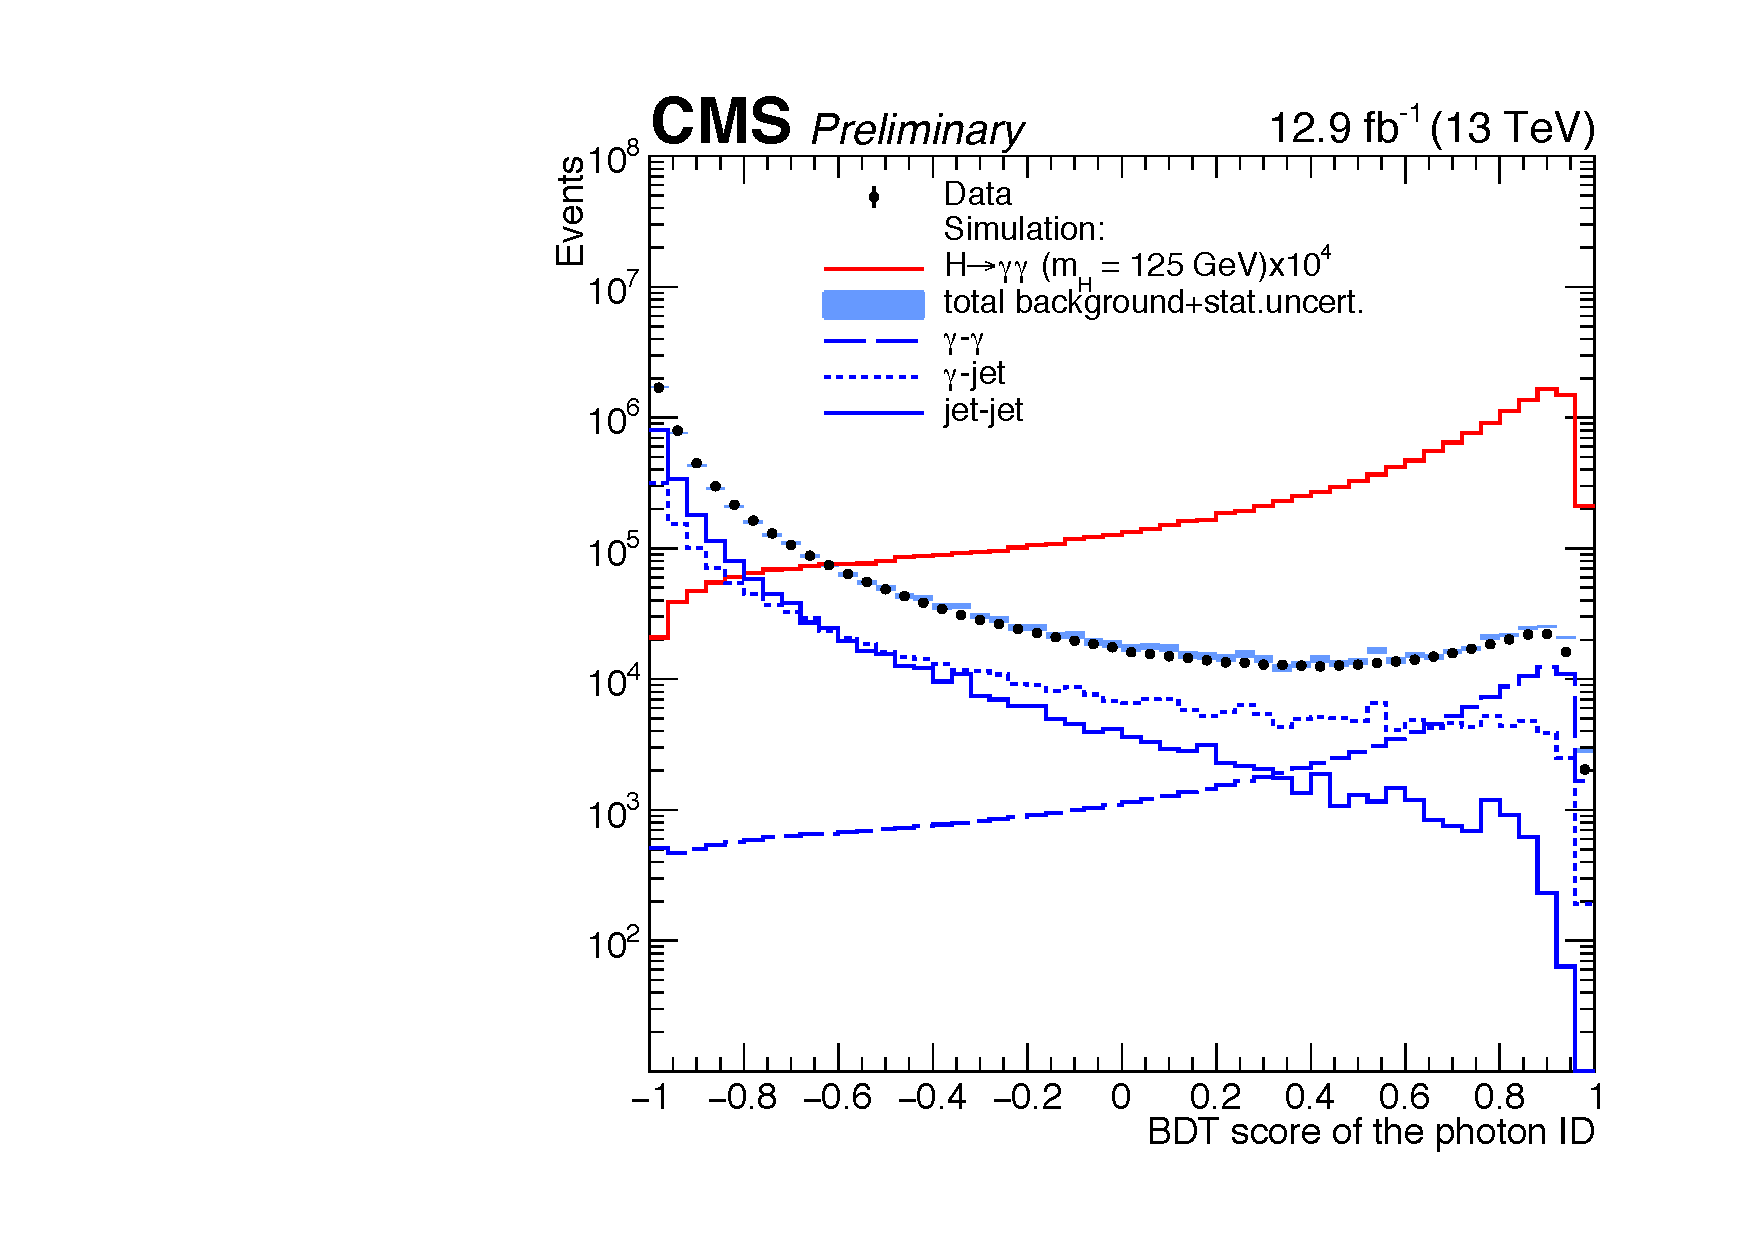
\includegraphics[width=0.5\textwidth]{recoFigures/\whichFig/validation_phoID.pdf}
\caption{
The \PhoIdBdt output score for the lower-scoring photon in each diphoton pair in the range $100 < m_{\gamma \gamma} < 180\GeV$ for data and simulation. The simulation is composed of signal (\Hgg photons with $\mH=125\GeV$) and background, which has been split into $\gamma$-$\gamma$, $\gamma$-$\textrm{jet}$ and $\textrm{jet}$-$\textrm{jet}$ components. The sum of the background components has been scaled to the number of events in data.}
\label{fig:reco:photon_id_score_hgg_bkg}
\end{figure}

\begin{figure}[hptb]
\centering 
%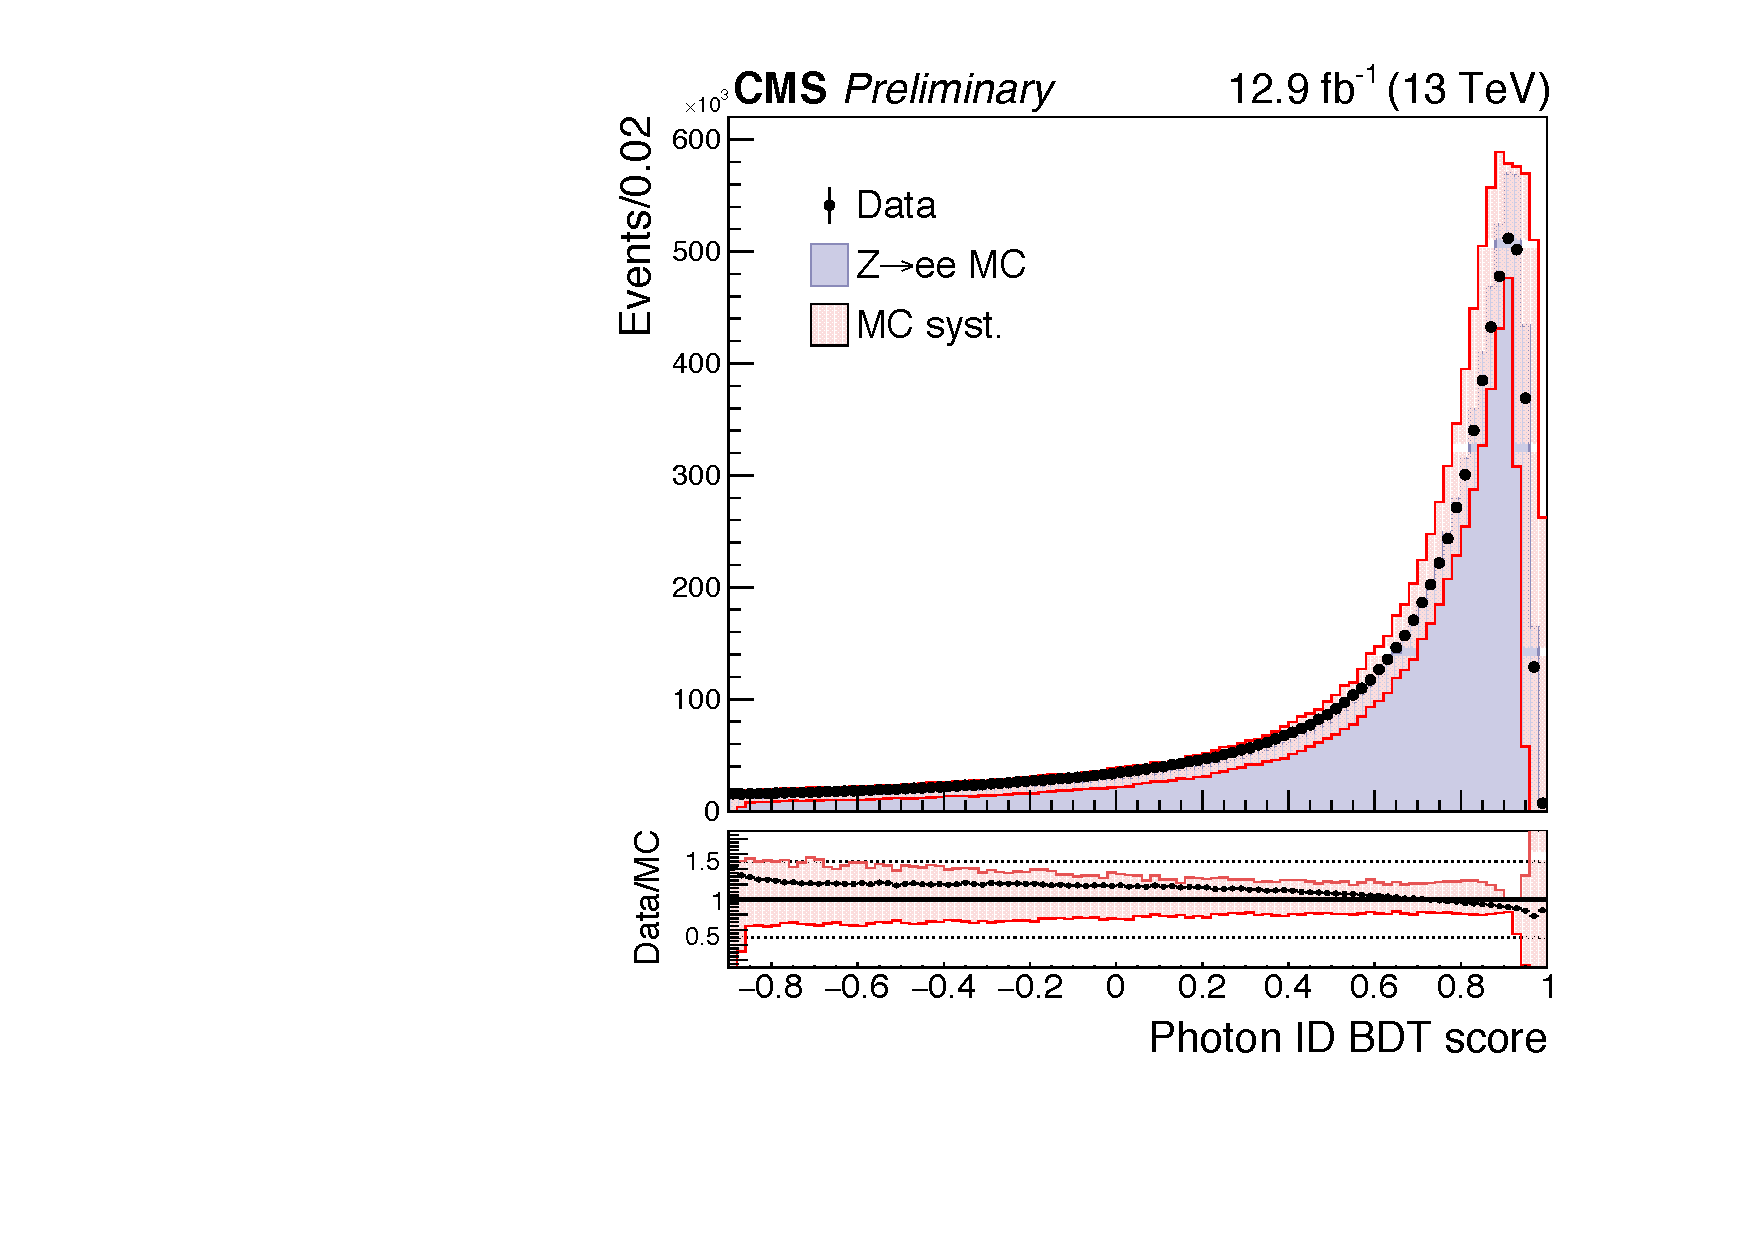
\includegraphics[width=0.53\textwidth]{recoFigures/idmva_syst_combined.pdf}
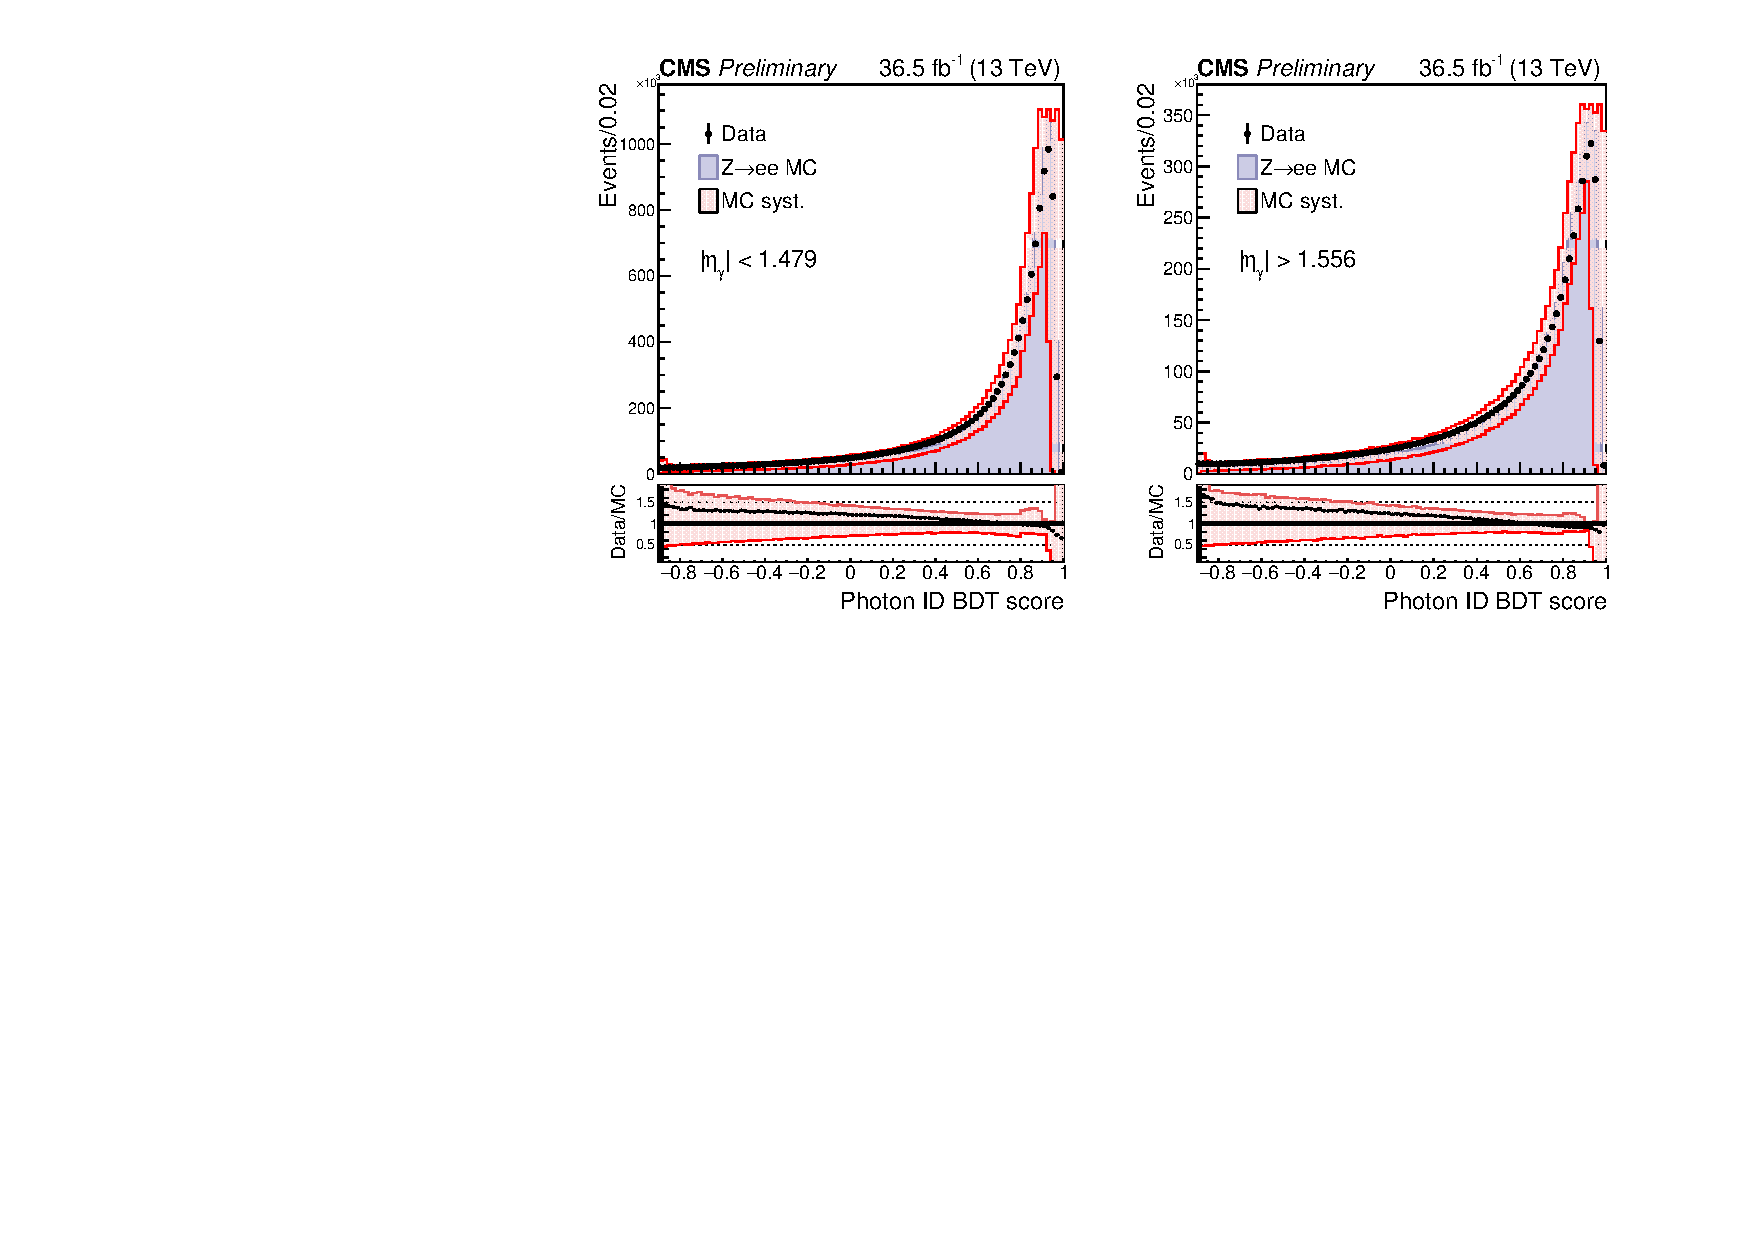
\includegraphics[width=\figWidth\textwidth]{recoFigures/\whichFig/idmva_syst.pdf}
\caption{ The \PhoIdBdt output score for \Zee events in data and simulation (labelled MC), where 
the electrons are reconstructed as photons with the electron veto requirement inverted. The red shaded region corresponds to a systematic uncertainty of approximately 3\% on the value of the output score, to cover discrepancies between data and simulation.}
\label{fig:reco:photon_id_zee_validation}
\end{figure}


\section{Vertex reconstruction}
\label{reco:sec:vertex}

\subsection{Vertex identification BDT}
As is discussed in \Sec~\ref{reco:sec:intro}, the determination of the location of Higgs decay is an important step in the reconstruction and selection of \Hgg events, as it impacts the calculation of the invariant mass of diphoton system. For events where the distance $\Delta z$ between the true vertex and the selected vertex in the $z$-direction is less than 1\cm, then the impact of the opening angle uncertainty on the mass resolution is negligible. Conversely, for events where $\Delta z>1\cm$ the \mgg distribution is wider, corresponding to a degradation of the mass resolution. %CITATION NEEDED?

Since the \CMS \ECAL is composed of a single layer of crystals, it cannot be used to point towards the vertex location. %Furthermore, unless a photon undergoes pair conversion, it does not leave any tracks in the tracker. 
None the less, it is possible to exploit tracks recoiling from the diphoton system and the tracks of any electrons resulting from pair conversion to help determine the location of the vertex.

The first step is to produce a list of candidate vertex locations by considering all the tracks recorded in the tracker and grouping them into common points of origin by determining their closest point of approach to the beamline. Next, a per-vertex \BDT is used to determine which of the candidate vertices is most likely to be the point of origin of the Higgs boson decay. This \BDT is referred to as \VtxIdBdt. The set of input variables is listed below, where $N_{tracks}^{vtx}$ is the number of charged \PF candidates associated with a given vertex, $\vec{\pT}^i$ is the transverse momentum of the $i^{\textrm{th}}$ candidate and $\vec{\pT}^{\gamma\gamma}$ is the transverse momentum of the diphoton system :
\begin{itemize}
\item the sum of squared transverse momenta of all tracks, $\sum_{i=0}^{N_{tracks}^{vtx}} | \vec{\pT}^{i} |^2$;
\item the recoil of the tracks relative to the diphoton system, $\sum_{i=0}^{N_{tracks}^{vtx}} (- \vec{\pT}^i \cdot \frac{\vec{\pT}^{\gamma\gamma}}{|\vec{\pT}^{\gamma\gamma}| })$;
\item the transverse momentum asymmetry, $\frac{(|\sum_{i=0}^{N_{tracks}^{vtx}} \vec{\pT}^i| - |\vec{\pT}^{\gamma\gamma}|)}{(|\sum_{i=0}^{N_{tracks}^{vtx}} \vec{\pT}^i| + |\vec{\pT}^{\gamma\gamma}|)}$.
\end{itemize}

Two additional variables are also considered if one of the two photons has converted into an $\Pep\Pem$ pair, where additional information is available to help identify the vertex:
\begin{itemize}
\item the number of converted photon candidates in the event;
\item the pull $|z_{vertex} - z_{conv}|/\sigma_{z_{conv}} $, where $z_{vertex}$ and $ z_{conv}$ are the $z$-components of the positions of the reconstructed vertex under consideration and the position of the vertex extrapolated from the conversion tracks respectively, and $\sigma_{z_{conv}} $ is the uncertainty on the extrapolated vertex position.
\end{itemize}

The \VtxIdBdt is trained using simulated Higgs boson events %with $\mH=126\GeV$, 
where the contribution from each production mode is weighted by the respective \SM \crosssection. Reconstructed vertices matched to a generator-level Higgs boson decay vertex are defined as the signal. All other reconstructed vertices not associated with a Higgs boson decay are treated as background. The training samples are reweighted to account for the fact that the width of the \emph{beamspot} (the distribution of reconstructed vertices as a function of longitudinal position) in data and simulation is not the same. This width is modelled as 5.1\cm in simulation but is measured to be 3.6\cm in the data samples used in this analysis. The reweighting is performed as a function of $\Delta z$. After the reweighting, the width of the distribution of $\Delta z$ in simulation matches the width of the $\Delta z$ distribution in data, which is the beamspot width multiplied by $\sqrt{2}$.

The \VtxIdBdt is validated for unconverted photons using \Zmumu events in data and simulation. After determining the vertex of the decay from the muon tracks, the events are re-reconstructed removing the muon tracks to mimic the \Hgg system. For converted photons, the \VtxIdBdt is validated using a similar technique with \gammaJet samples, where the vertex is obtained from the tracks associated with the jet, and the events are re-reconstructed removing the tracks associated with the jet to imitate a diphoton system. The vertex-finding efficiencies as a function of \pT and as a function of the number of vertices in \Zmumu and \gammaJet events can be seen in \Fig~\ref{fig:reco:vtx_id_eff_zmumu_validation} and \Fig~\ref{fig:reco:vtx_if_eff_gjet_validation}. %The data sample was obtained by triggering on isolated muon tracks with $\pT > 27\GeV$, requiring tight identification criteria for both muons, and selecting events where the invariant mass of the dimuon system was between 70\GeV and 110\GeV. A simulated sample of \Zmumu events is used for this study, where the events have been re-weighted such that their \PU distribution matches that of the data and the beamspot reweighting discussed in \Sec~\ref{} is applied. The differences between the data and simulation are used to estimate the systematic uncertainties associated with the choice of vertex. %and \gammaJet
\begin{figure}
\begin{center}
%\includegraphics[width=0.45\linewidth]{vtxIdFig/eff_pt_Zmumu.pdf}
%\includegraphics[width=0.45\linewidth]{vtxIdFig/eff_nVtx_Zmumu.pdf}
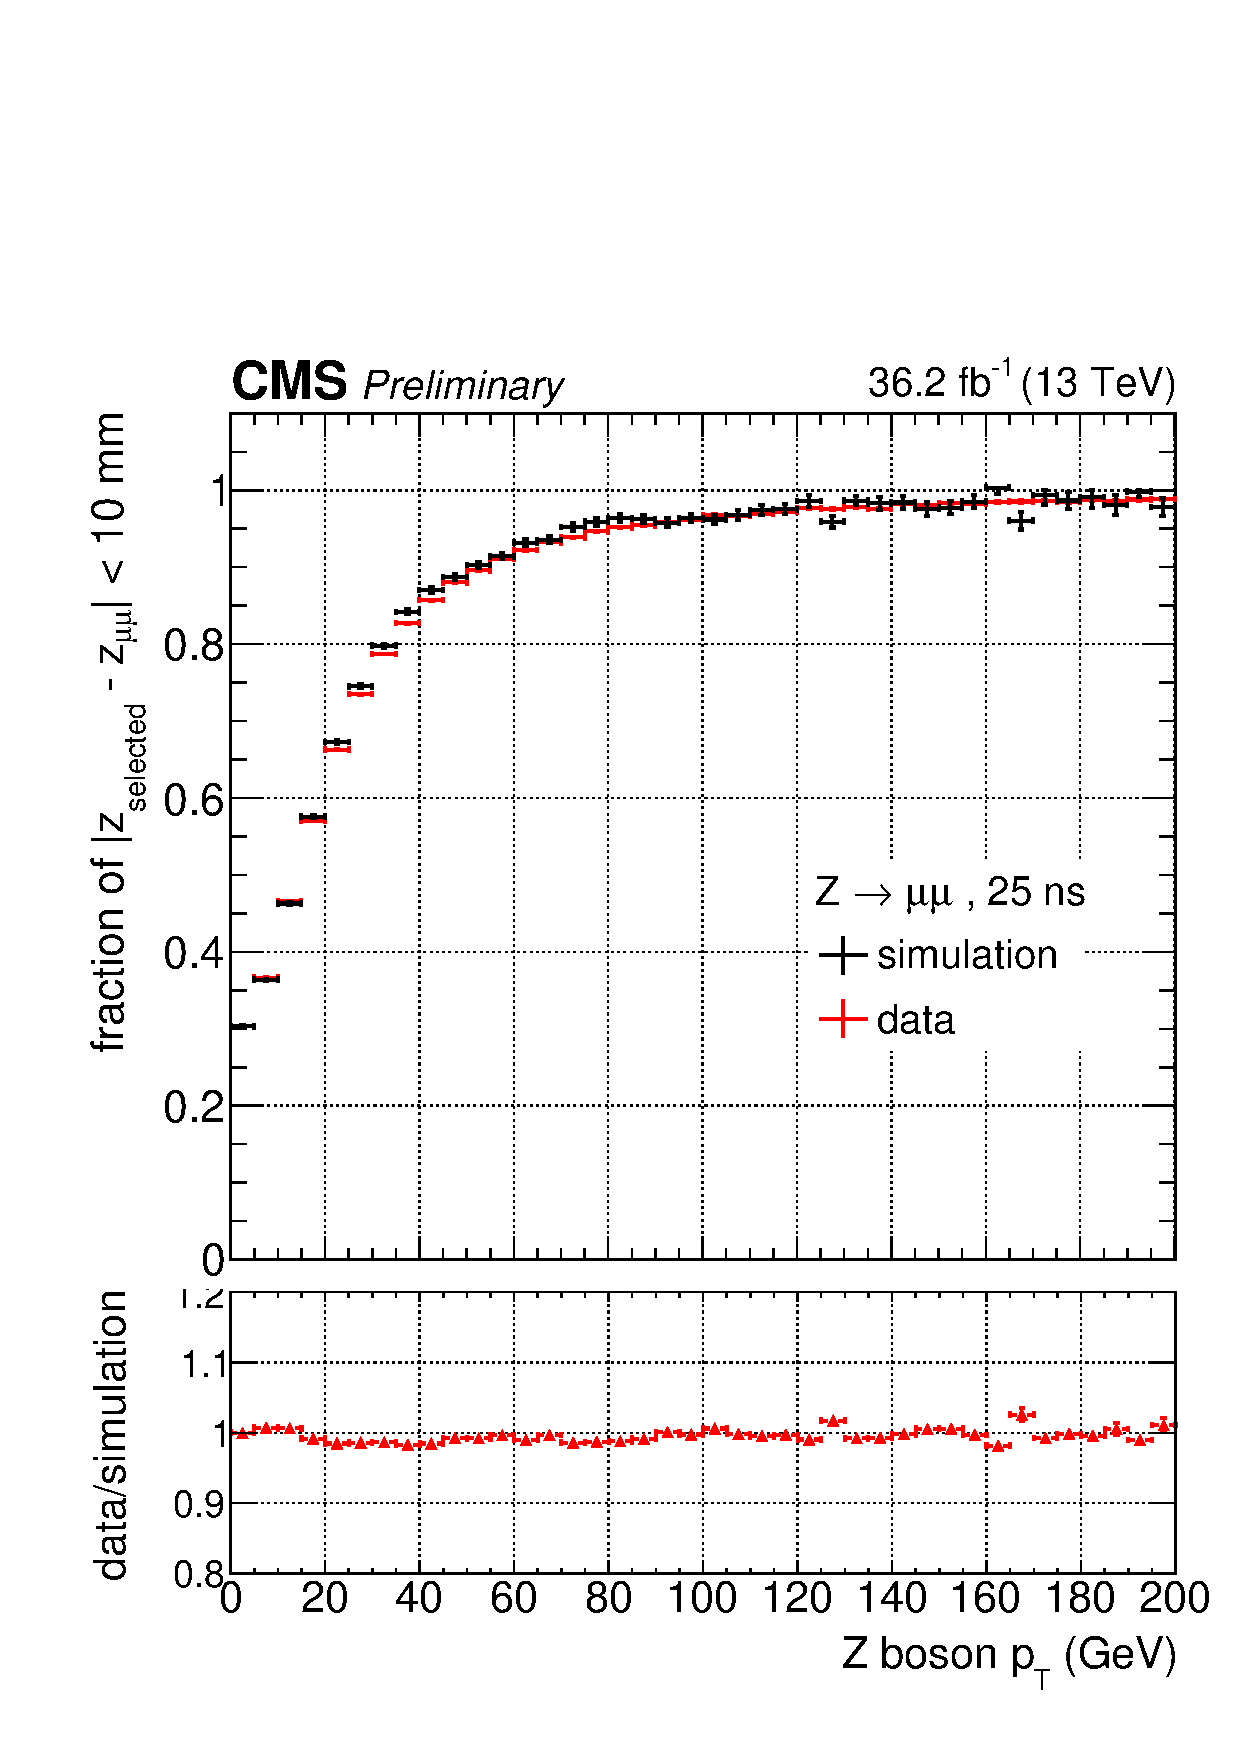
\includegraphics[width=0.49\linewidth]{recoFigures/\whichFig/Zmumu_eff_vs_pt.pdf}
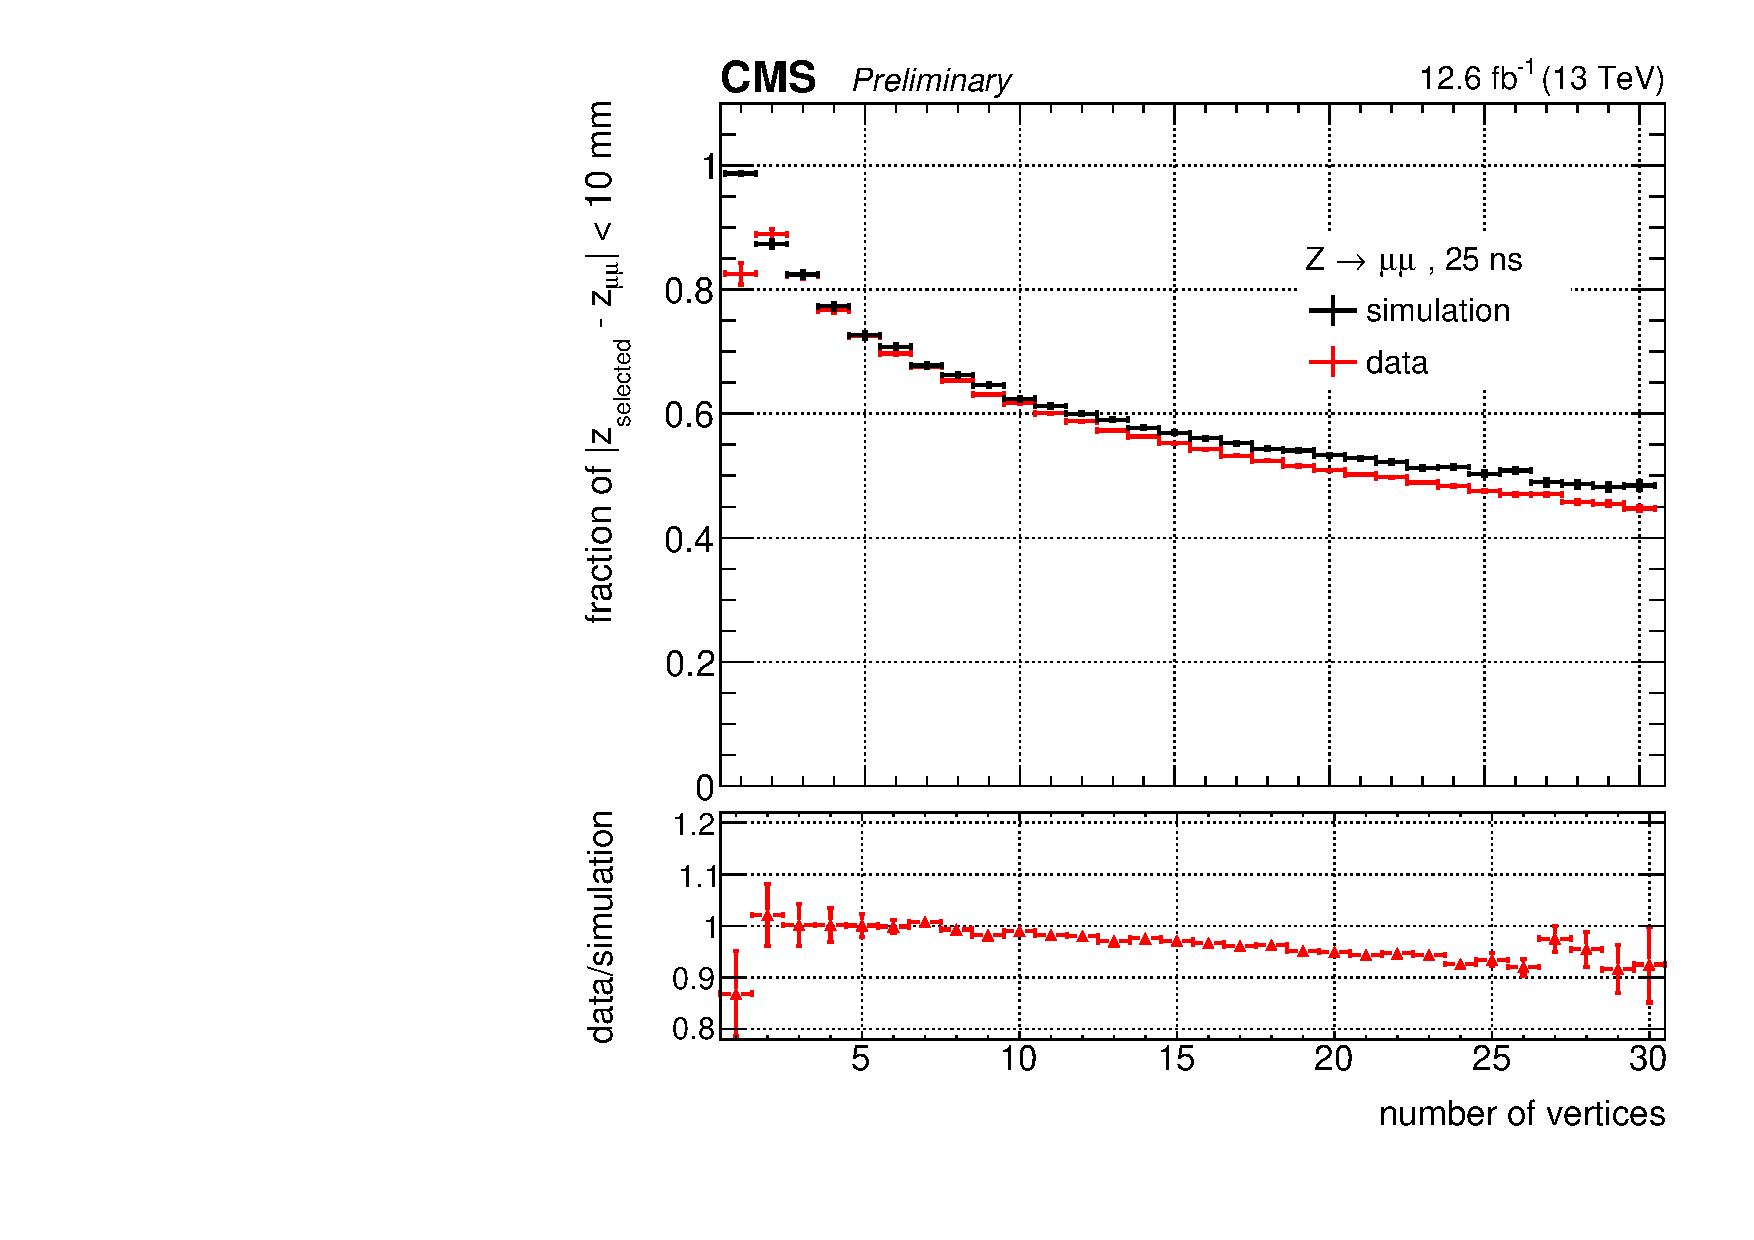
\includegraphics[width=0.49\linewidth]{recoFigures/\whichFig/Zmumu_eff_vs_nVtx.pdf}
\caption{The efficiency of selecting a vertex within 1\cm of the true vertex in \Zmumu events, as a function of the \pT of the $\PZ$-boson (left) and as a function of the number of vertices (right) in the event.}
\label{fig:reco:vtx_id_eff_zmumu_validation}
\end{center}
\end{figure}

\begin{figure}
\begin{center}
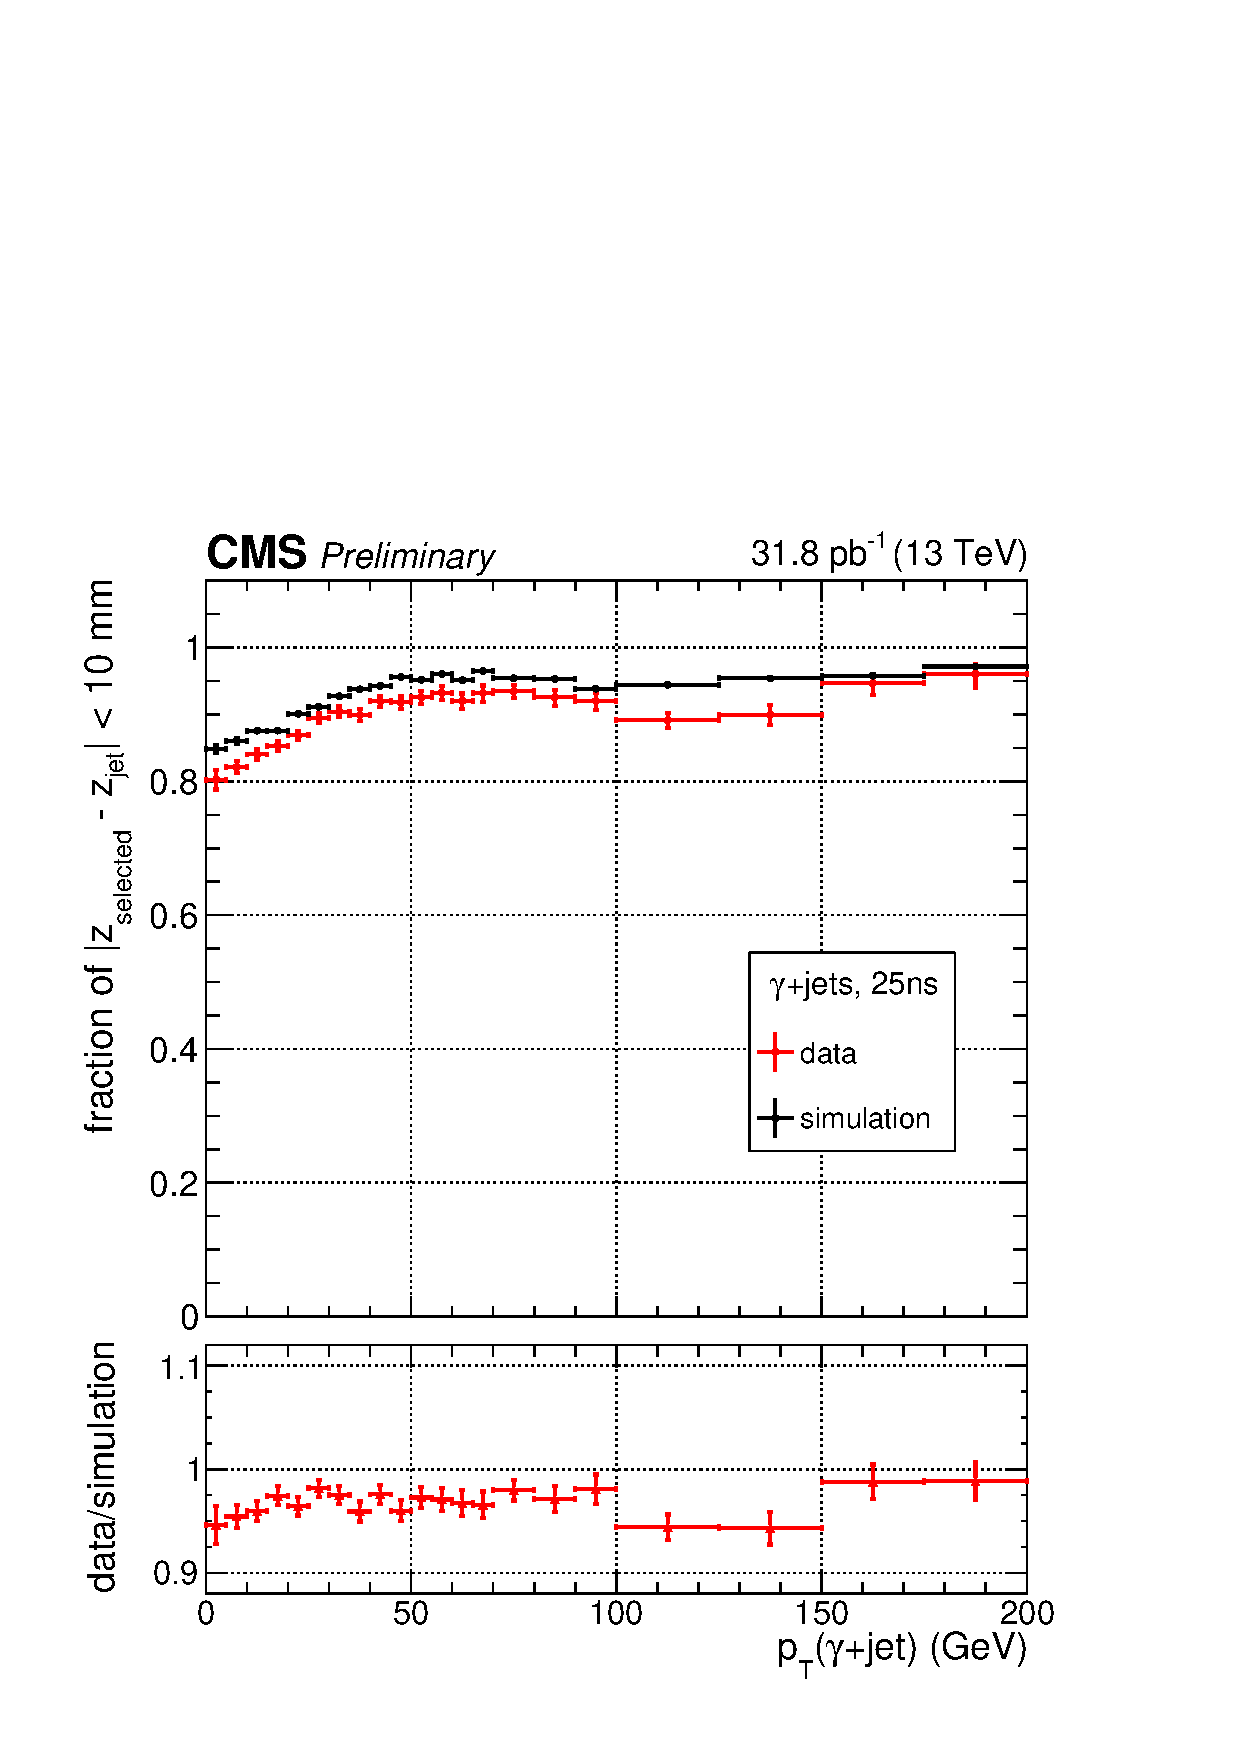
\includegraphics[width=0.49\linewidth]{recoFigures/\whichFig/GammaJets_eff_vs_pT.pdf}
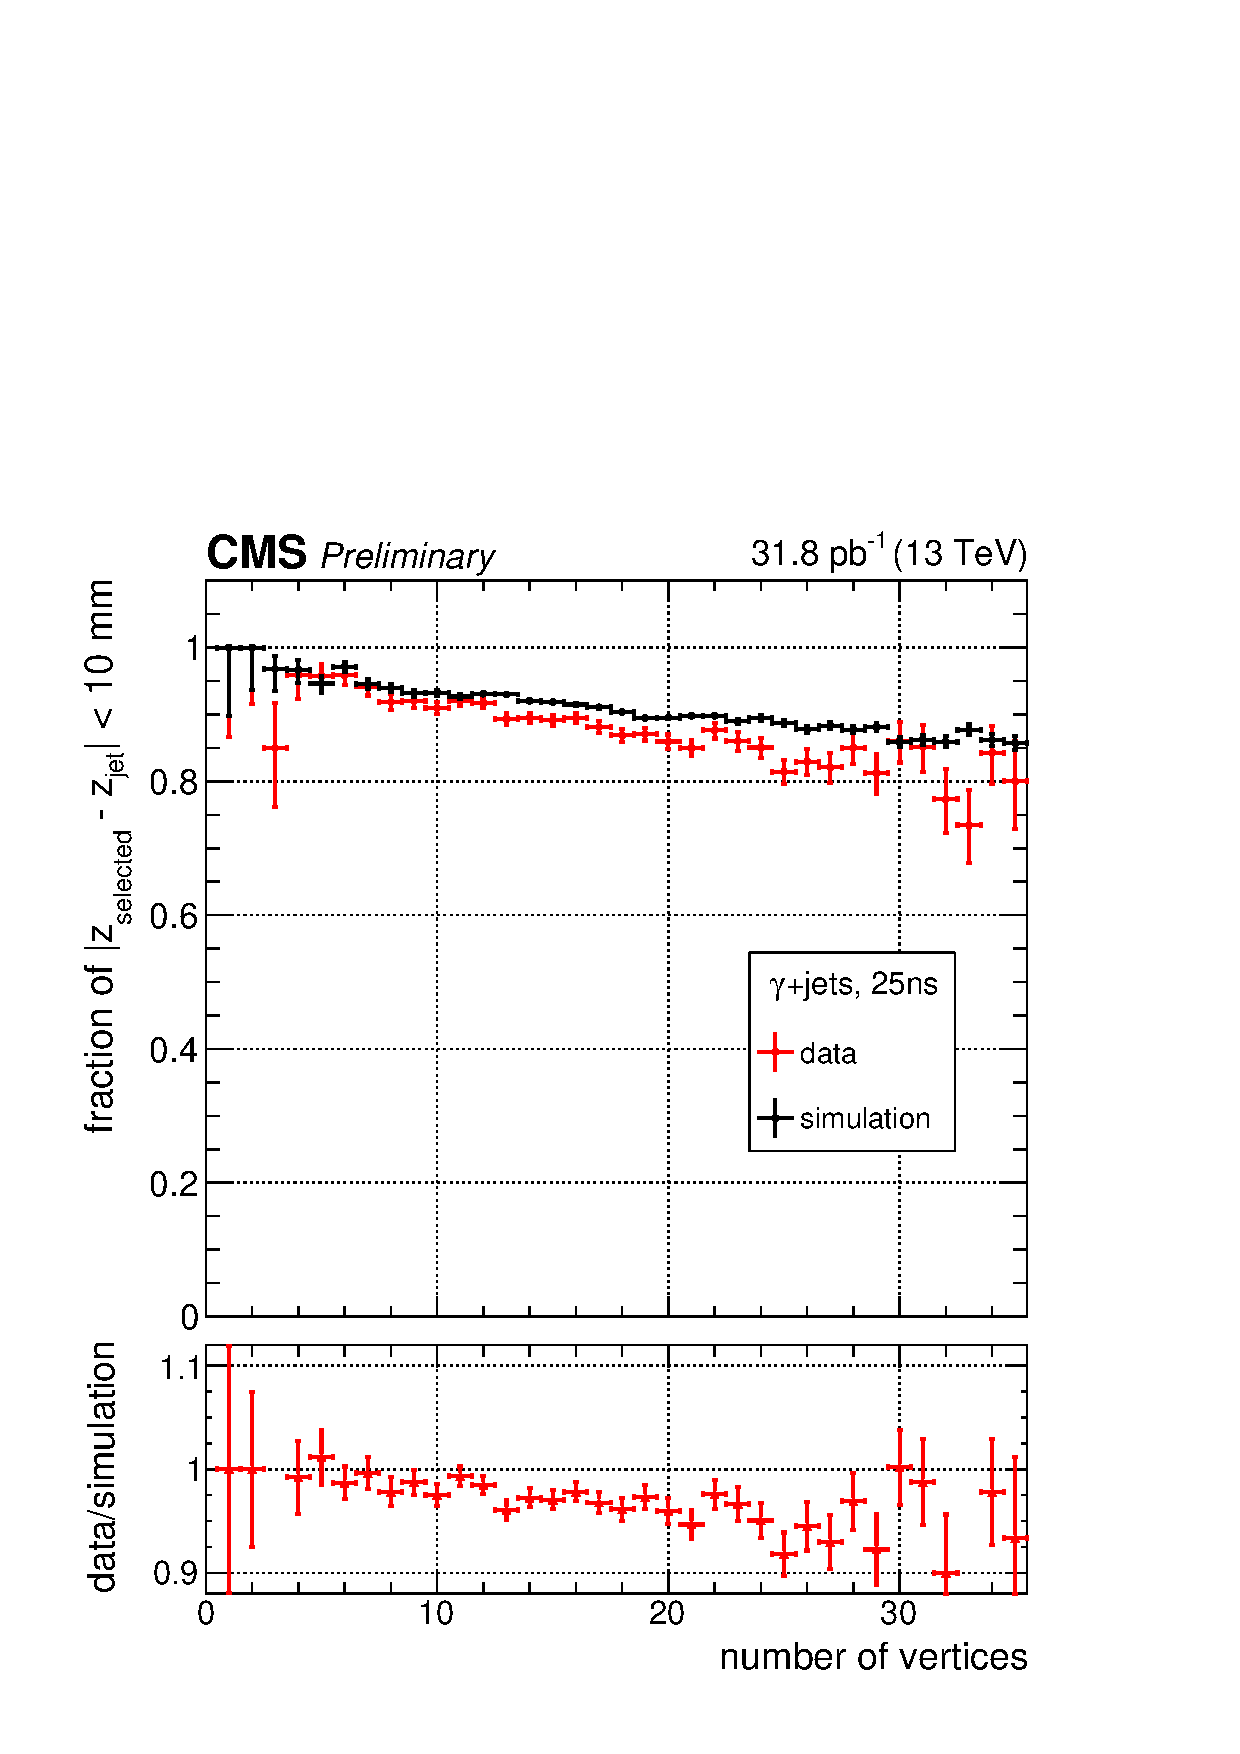
\includegraphics[width=0.49\linewidth]{recoFigures/\whichFig/GammaJets_eff_vs_nVtx.pdf}
\caption{The efficiency of selecting a vertex within 1\cm of the true vertex in \gammaJet events, as a function of the \pT of the \gammaJet system (left) and as a function of the number of vertices (right) in the event.}
\label{fig:reco:vtx_if_eff_gjet_validation}
\end{center}
\end{figure}


The efficiency of the \VtxIdBdt to select the right vertex within 1\cm of the true one is estimated in simulated signal events ($\mH=125\GeV$), shown as a function of the number of vertices in the event and as a function of \pT in \Fig~\ref{fig:reco:vtxidbdt_eff}. The average efficiency is of the order of 80\%. 

\begin{figure}[hpt]
\centering
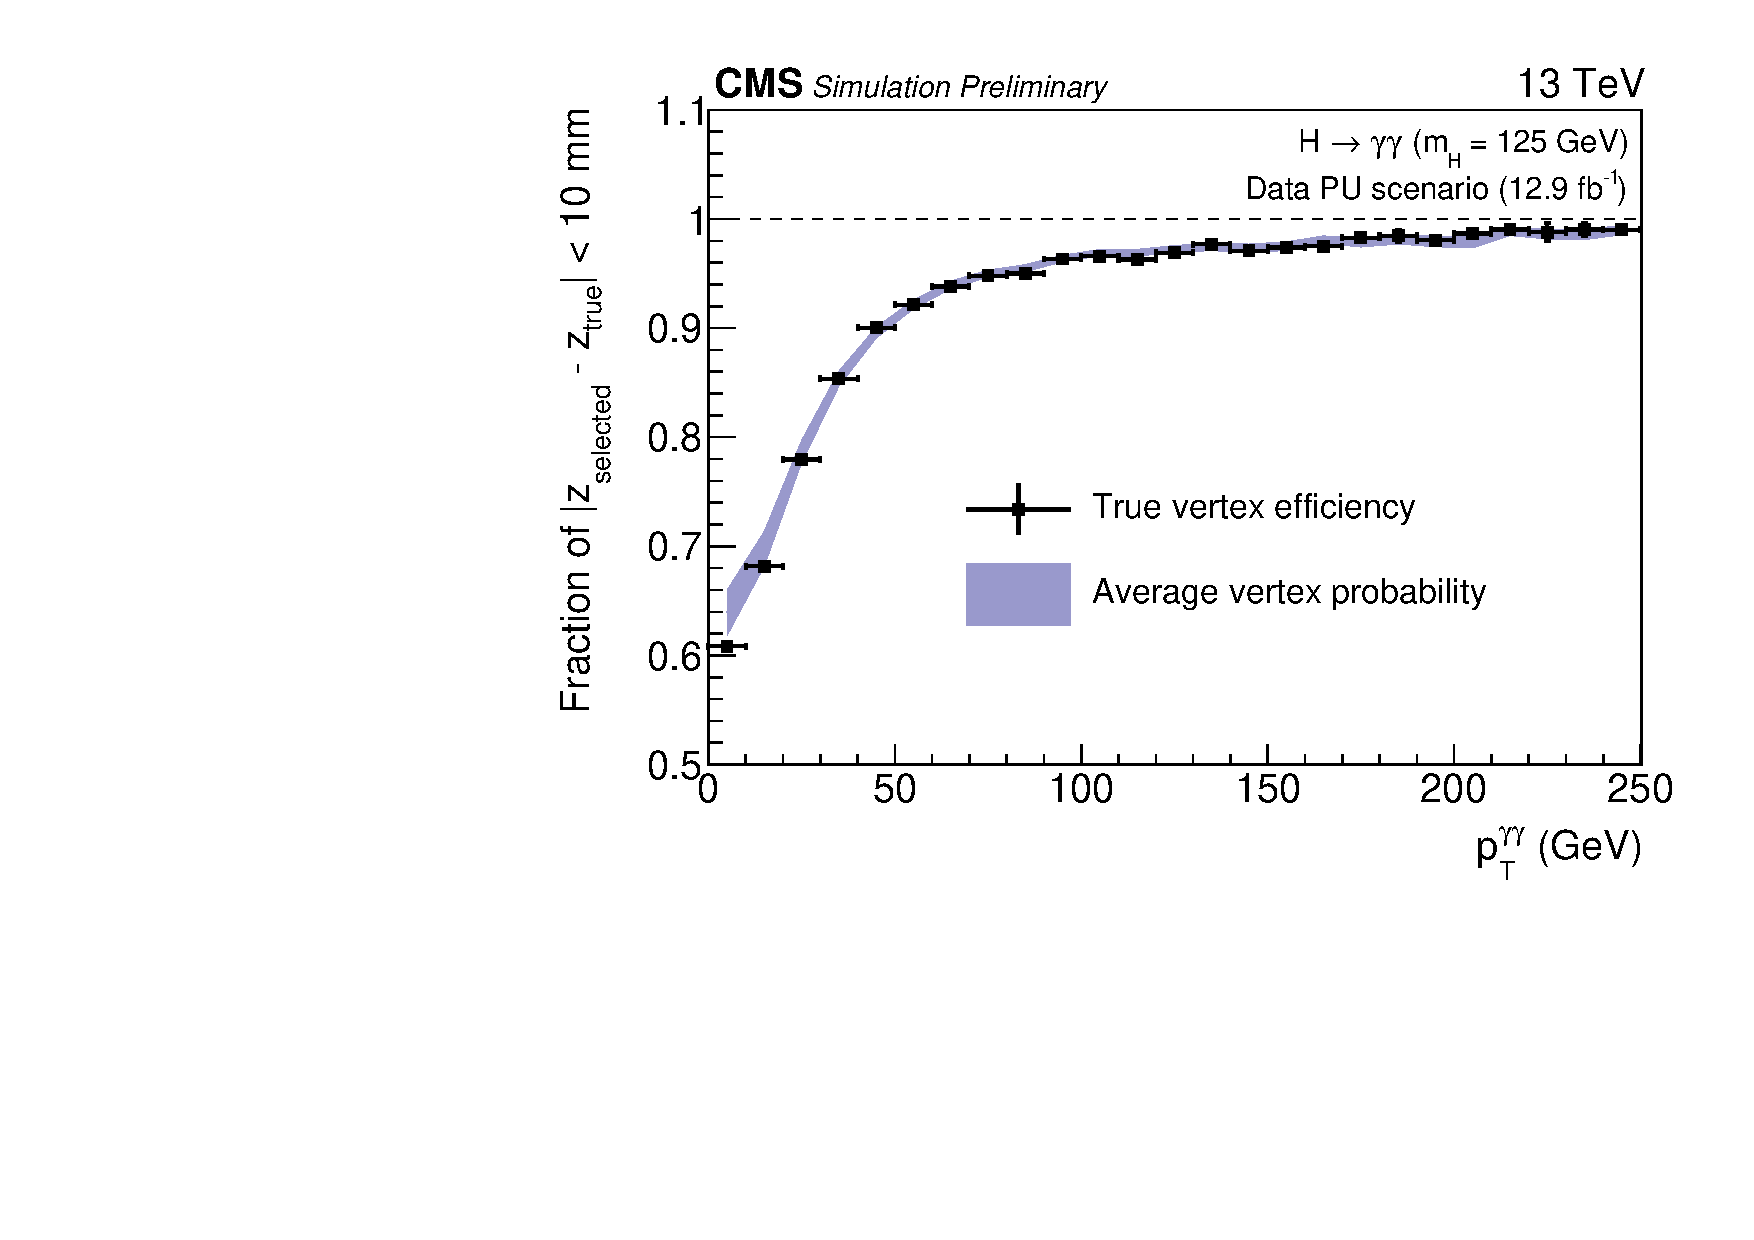
\includegraphics[width=0.7\textwidth]{recoFigures/\whichFig/PtBSReweighted.pdf}\\
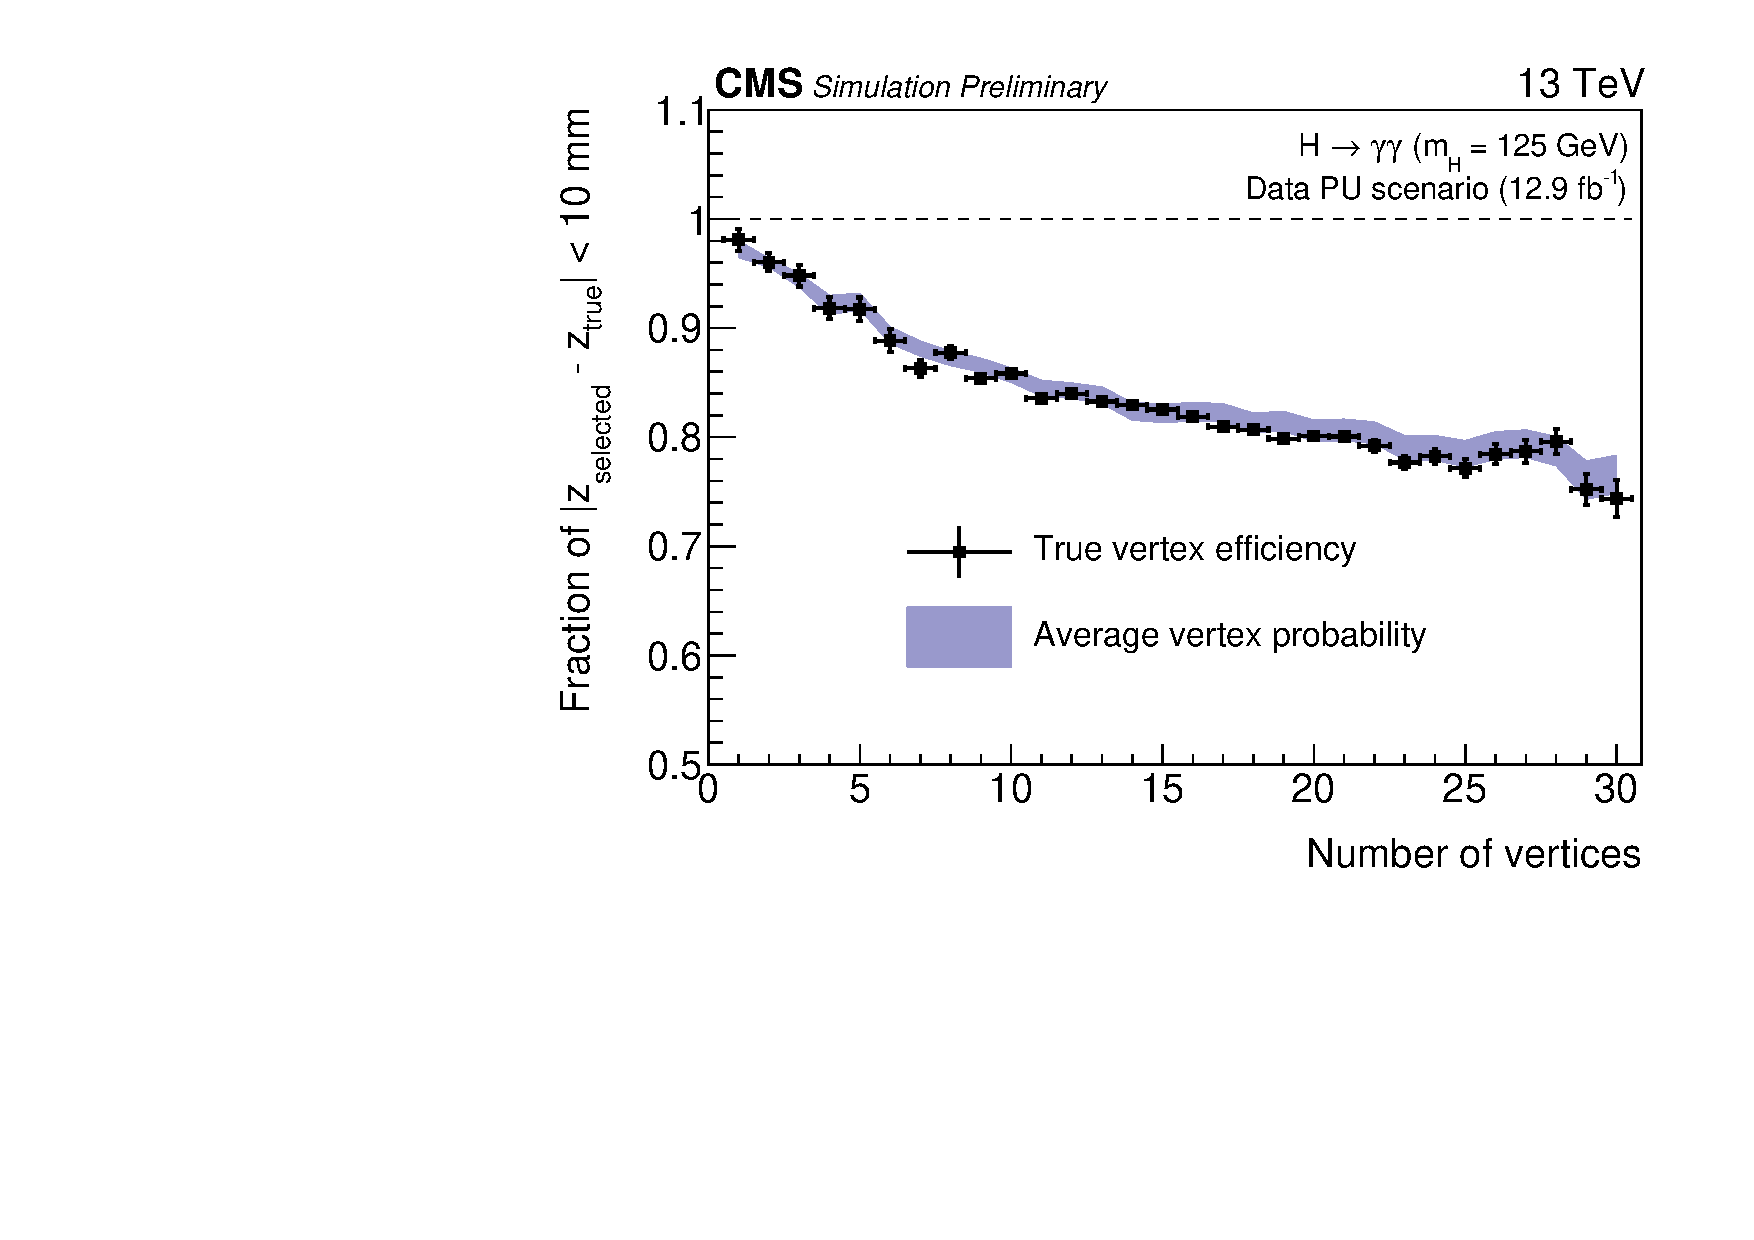
\includegraphics[width=0.7\textwidth]{recoFigures/\whichFig/NvtxBSReweighted.pdf}
\caption{The efficiency to select a vertex within 1\cm of the true vertex in simulated \Hgg events as a function \pT and the number of vertices in the event. The estimated probability that the vertex is chosen within 1\cm is superimposed. The uncertainty on the vertex-finding probability is determined using \Zmumu events. The simulation is reweighted such that the distribution of the number of vertices and the width of the interaction region matched in data and simulation. }
\label{fig:reco:vtxidbdt_eff}
\end{figure}

\subsection{Correct vertex probability BDT}
\label{reco:sec:vtx_prob}
%If the chosen vertex is over 1\cm away from the true one, the invariant mass resolution is dominated by the uncertainty on the vertex position. It is therefore desirable to have a per-event estimate of how likely it is that the vertex is chosen within 1\cm of the true one. This is referred to as the \emph{correct vertex probability}. This information is used to categorise events by sensitivity, as described in \Sec~\ref{cat:sec:dipho_bdt}.

An additional \BDT, labelled \VtxProbBdt, is used to estimate of the per-event probability that the correct vertex was chosen by the \VtxProbBdt, which is used as an input to the event classification \BDT described in \Sec~\ref{cat:sec:dipho_bdt}. The \VtxProbBdt is trained on simulated \Hgg events and uses the following input variables: 

\begin{itemize}
\item the number of reconstructed vertices in the event;
\item the \pT of the diphoton system;
\item the output scores of the three vertices ranked highest by the \VtxIdBdt;
\item the distance in the $z$-direction between the first- and second-highest ranked vertices;
\item the distance in the $z$-direction between the first- and third-highest ranked vertices;
\item the number of converted photons in the diphoton. 
\end{itemize}

The correct vertex probability is parametrized by a $4^{th}$-order polynomial as a function of \VtxIdBdt output score. This is done separately for converted and unconverted photons. The estimated correct vertex identification probability is shown on the same plot as the vertex efficiency measured in simulation in \Fig~\ref{fig:reco:vtxidbdt_eff}. The \VtxProbBdt is validated using \Zmumu and \gammaJet events. 

\section{Reconstruction of other particles} 
\label{reco:sec:other}
\subsection{Electrons}

%In the study of the \Hgg decay, electrons are used in two ways. Firstly, they are used to validate reconstruction and selection algorithms using \Zee events. Secondly, they 
\ifNewAnalysis
Electrons are used for the categorisation of \Hgg events where the Higgs boson events are produced by the \ZH or \WH mechanism. 
\else
Electrons are used for the categorisation of \Hgg events where the Higgs boson events are produced by the \ttH mechanism. 
\fi
Candidate \PF electrons are reconstructed either starting from \ECAL deposits which are matched to tracks (called \emph{ECAL-driven} electrons), or starting from tracks which are matched to \ECAL deposit (called \emph{tracker-driven} electrons). Typically, energetic and isolated electron candidates will be reconstructed as \ECAL-driven, while low-energy ($\pT \lesssim 10\GeV$) electrons will be reconstructed as tracker-driven. Electrons from both seeding algorithms are eventually grouped together to form the set of \PF electron candidates. The electrons used in this thesis originate from \PWpm or \PZ decays, and hence are mostly ECAL-driven.

The ECAL-driven electrons are obtained via a procedure analogous to that described for photons in \Sec~\ref{reco:sec:photons}, but with the additional step of associating a track based on geometrical requirements. Candidate tracks are obtained from tracker hits within some window in $z$ and $\phi$ around the \SC position. The tracks are fitted with a special algorithm which accounts for changes in direction caused by the emission of bremsstrahlung. The \SC is associated to the track whose extrapolated position in the \ECAL is nearest to the energy-weighted position of the \SC, but requiring that the distance in the $\eta$-direction ($\phi$-direction) be no more than $0.02$ (0.15). The energy of electrons is obtained from the \SC energy, where the final energy correction $F_{SC}$ is obtained using a \BDT method analogous to that described in \Sec~\ref{sec:reco:photon:phoenergybdt}, but specially trained for electron candidates.

\subsection{Muons}

\ifNewAnalysis
Muons are used for the selection of Higgs bosons which are produced by the \ZH or \WH mechanism. 
\else
Muons are used for the selection of Higgs bosons which are produced by the \ttH mechanism. 
\fi
Muons are constructed by geometrically matching tracks reconstructed independently in the tracking system and in the muon chambers. Muon candidates must have some hits in both \subdetector\s to qualify as \PF muons: this helps to avoids cases where cosmic rays or muons produced in jets are misreconstructed as muons from the hard scattering interaction~\cite{MuonReco}.

\subsection{Jets}
\label{reco:sec:jets}

Gluons or quarks exiting the \pp interaction hadronize, forming collimated \emph{jets} of charged and neutral hadrons.
In the \Hgg analysis, jets are used to identify events where the Higgs boson is produced by the \VBF process. 
Jets are reconstructed using the \antiKt algorithm~\cite{antiKt} from \PF candidates, using a cone of radius $R=0.4$. Jets originating from \PU can sometimes overlap with jets which originate from particles produced in the hard scattering interaction. To mitigate this effect, \PFCHS is used. In this scheme, the \PF charged hadron candidates associated to a vertex other than the vertex selected by the procedure described in \Sec~\ref{reco:sec:vertex} are ignored during the jet reconstruction. %Events can have multiple possible photon pairs ans since each photon pair is associated with a vertex, the event can have potentially multiple possible selected vertices. The collection of jets is therefore reclustered using the \PFCHS under all possible selected vertex scenarios. 
\ifNewAnalysis
An algorithm called \PUJID is used to remove jets which did not originate from the hard scatter. The algorithm is developed centrally by the \CMS collaboration, and uses variables related to the following quantities: the width of the jet; the number of vertices in the event; the multiplicities of the constituent particles; and the \pT of the leading particle of the jet compared to the total jet \pT. In the tracker acceptance is $|\eta|<2.5$, additional information about the number of charged particles in the jet and the proportion of tracks origination from the \PV can be used. A selection is made on the output score of the \PUJID for different bins in \pT and $\eta$, which keeps approximately $80\%$ of genuine jets from the hard scatter while rejecting approximately $99\%$ of \PU jets within the tacker acceptance, and between $75\%$ and $30\%$ of \PU jets outside of tracker acceptance, depending on the jet's location in $\eta$.
\else
Since the tracker acceptance is $|\eta|<2.5$, no \PF charged hadron candidates are available outside this range, so \PFCHS has no effect. For the jets reconstructed outside this region, but still in acceptance, a different \PU mitigation technique is used using a selection on the width of the jet. 
The width of the jet is described by the variable $\RMS= \sum_{\text{PF candidates}}\pT^2 \Delta R^2/ \sum_{\text{PF candidates}}\pT^2 $, where $\Delta R$ is the distance between the \PF candidate and the jet axis from the cone. Jets must have $\RMS<0.03$ to pass the \PU mitigation requirement. 
\fi
Finally, all jets are required to be within $|\eta|<4.7$.

Parametric corrections to the energy of the jets are made to account for the additional energy of \PF neutral hadrons from \PU which are included in jets and the nonuniformity of the detector response.

\ifNewAnalysis
\subsection{Missing energy}

Certain particles,such as neutrinos, do not leave any deposits in the detector, and therefore carry away a certain amount of energy which cannot be reconstructed. This results in an imbalance in the sum of transverse momentum. The amount of \MET is calculated by considering the magnitude and direction of \pT required to balance all the jets and \PF objects in an event. Reconstructed \MET is used to identify decays from $\PWpm$ bosons, for example when identifying Higgs boson decays originating from the \WH production mode.\fi


  \chapter{Event categorisation}
\label{chap:categorisation}

\section{Introduction}
\label{cat:sec:intro}

The basic experimental method for the observation of the \Hgg decay is to search for a resonance above the diphoton continuum background. The sensitivity of this method is enhanced by the categorisation of events according to their expected signal-to-background ratio. Furthermore the use of additional particles in the event allows the measurement of the cross-section of each production mode individually, thus probing the strength of the Higgs boson's interaction with different types of particle. %These considerations motivate the following categorisation scheme. 

The most common production mode, \ggH, produces a Higgs boson in isolation. This leaves only the photons resulting from \Hgg decay in the final state. The other production modes (\VBF, \VH and \ttH) produce the Higgs boson accompanied by additional particles. The \VBF mode has two quarks in the final state, which hadronize to form jets. The \VH mode produces a Higgs boson in association with a \PW or \PZ boson, which then decays to charged leptons, neutrinos or quarks, leading to reconstructed leptons, \MET or jets. Finally, the \ttH mode produces the Higgs boson in association with two top quarks, which decay to bottom quarks and either hadrons or leptons. These reconstructed additional particles can be used to categorise events. 

The \BDT used for categorisation of diphoton events is described in \Sec~\ref{cat:sec:dipho_bdt}. 
\ifNewAnalysis
The categorisation of \VBF, \VH and \ttH events is then discussed in \Sec\s~\ref{cat:sec:vbftag},~\ref{cat:sec:vhtag} and~\ref{cat:sec:tthtag}. 
\else
The categorisation of \VBF and \ttH events is then discussed in \Sec\s~\ref{cat:sec:vbftag} and~\ref{cat:sec:tthtag}. This analysis does not have any categories which specifically target \VH events.
\fi
Finally, the inclusive categories and the categorisation hierarchy are respectively discussed in \Sec\s~\ref{cat:sec:untagged} and~\ref{cat:sec:hierarchy}.

\section{Diphoton BDT}
\label{cat:sec:dipho_bdt}

For events reconstructed and selected as described in Chapter~\ref{chap:reconstruction}, a \BDT referred to as \DiPhoBdt is used rank diphotons by their expected signal-to-background ratio. The \DiPhoBdt is required to assess diphotons independently of their invariant mass, otherwise the \mH value of the training sample would introduce a bias in the output score. The input variables for the \DiPhoBdt are therefore chosen to be uncorrelated with the invariant mass of the diphoton system:

\begin{itemize}
\item the transverse momentum of each photon divided by $\mgg$; %to remove the correlation with \mH;
\item the $\eta$-position of each photon;
\item the \PhoIdBdt output score of each photon;
\item $\cos(\Delta\phi)$, the cosine of the angle between the photons in the $\phi$-direction;
\item \sigmarv, the per-event estimated mass resolution of the diphoton, assuming that the correct vertex was identified;
\item \sigmawv, the per-event estimated mass resolution of the diphoton, assuming that the vertex was not correctly identified;
\item $p_{rv}$, the per-event estimate of the probability that the correct vertex was chosen, calculated using the \VtxProbBdt described in \Sec~\ref{reco:sec:vtx_prob}.
\end{itemize}

The per-event estimated mass resolutions are calculated from the individual photon energy resolution estimates, labelled $\sigma^E_{\gamma_1}/E_{\gamma_1}$ and $\sigma^E_{\gamma_2}/E_{\gamma_2}$, which are given by the semiparametric regression \PhoEnergyBdt described in \Sec~\ref{sec:reco:photon:phoenergybdt}. If the vertex was correctly identified, the dominant contributions to the uncertainty on the mass resolution are the energy resolutions of each photon. Assuming Gaussian resolution functions, \sigmarv can be obtained by simply adding the individual relative photon energy resolutions in quadrature:
\begin{equation}
\sigmarv= \frac{1}{2} \sqrt{({\sigma^E_{\gamma_1}}/{E_{\gamma_1}})^2 +({\sigma^E_{\gamma_2}}/{E_{\gamma_2}})^2 }.
\end{equation} 
However, if the vertex was incorrectly identified, the uncertainty on the opening angle contributes significantly to the mass resolution. The effect is modelled by including an additional term which represents the uncertainty on the mass due to the uncertainty on the vertex position, labelled $\sigma^V_{\gamma\gamma}$. The distance between the true vertex and the selected vertex in the $z$-direction follows a Gaussian distribution which has a width equal to the width in $z$ of the beamspot multiplied by $\sqrt{2}$. Given the spatial positions of the photons, $\sigma^V_{\gamma\gamma}$ can therefore be calculated explicitly, and included in the sum in quadrature:
\begin{equation}
\sigmawv= \sqrt{(\sigmarv)^2 +(\sigma^V_{\gamma\gamma}/\mgg)^2 }.
\end{equation} 

The \DiPhoBdt is trained on simulated samples of signal and background processes. For the signal samples, events from different productions modes (all with $\mH=125\GeV$) are mixed according to their \SM cross-sections. The signal events used for training are also re-weighted by a factor $w^{\text{sig}}$ given by: 
\begin{equation}
w^{\text{sig}}= \frac{p_{rv}}{\sigmarv}+\frac{1-p_{rv}}{\sigmawv},
\end{equation} 
which codifies the fact that the signal-to-background ratio is inversely proportional to the mass resolution. This step ensures that the \DiPhoBdt gives a high score to events with good mass resolution.
The background for the training is composed of simulated diphotons originating from the irreducible and reducible \SM background processes. 

\Fig~\ref{fig:cat:diphobdt_a} shows the transformed \DiPhoBdt output score for signal and background events in the range $100 < \mgg < 180\GeV$. The transformation is applied to the \DiPhoBdt output score to give a flat distribution for signal events. The transformed \DiPhoBdt output score is validated using \Zee events in data and simulation, as can be seen in \Fig~\ref{fig:cat:diphobdt_b}.
\begin{figure}[hpt]
\centering
 \subfloat[]{
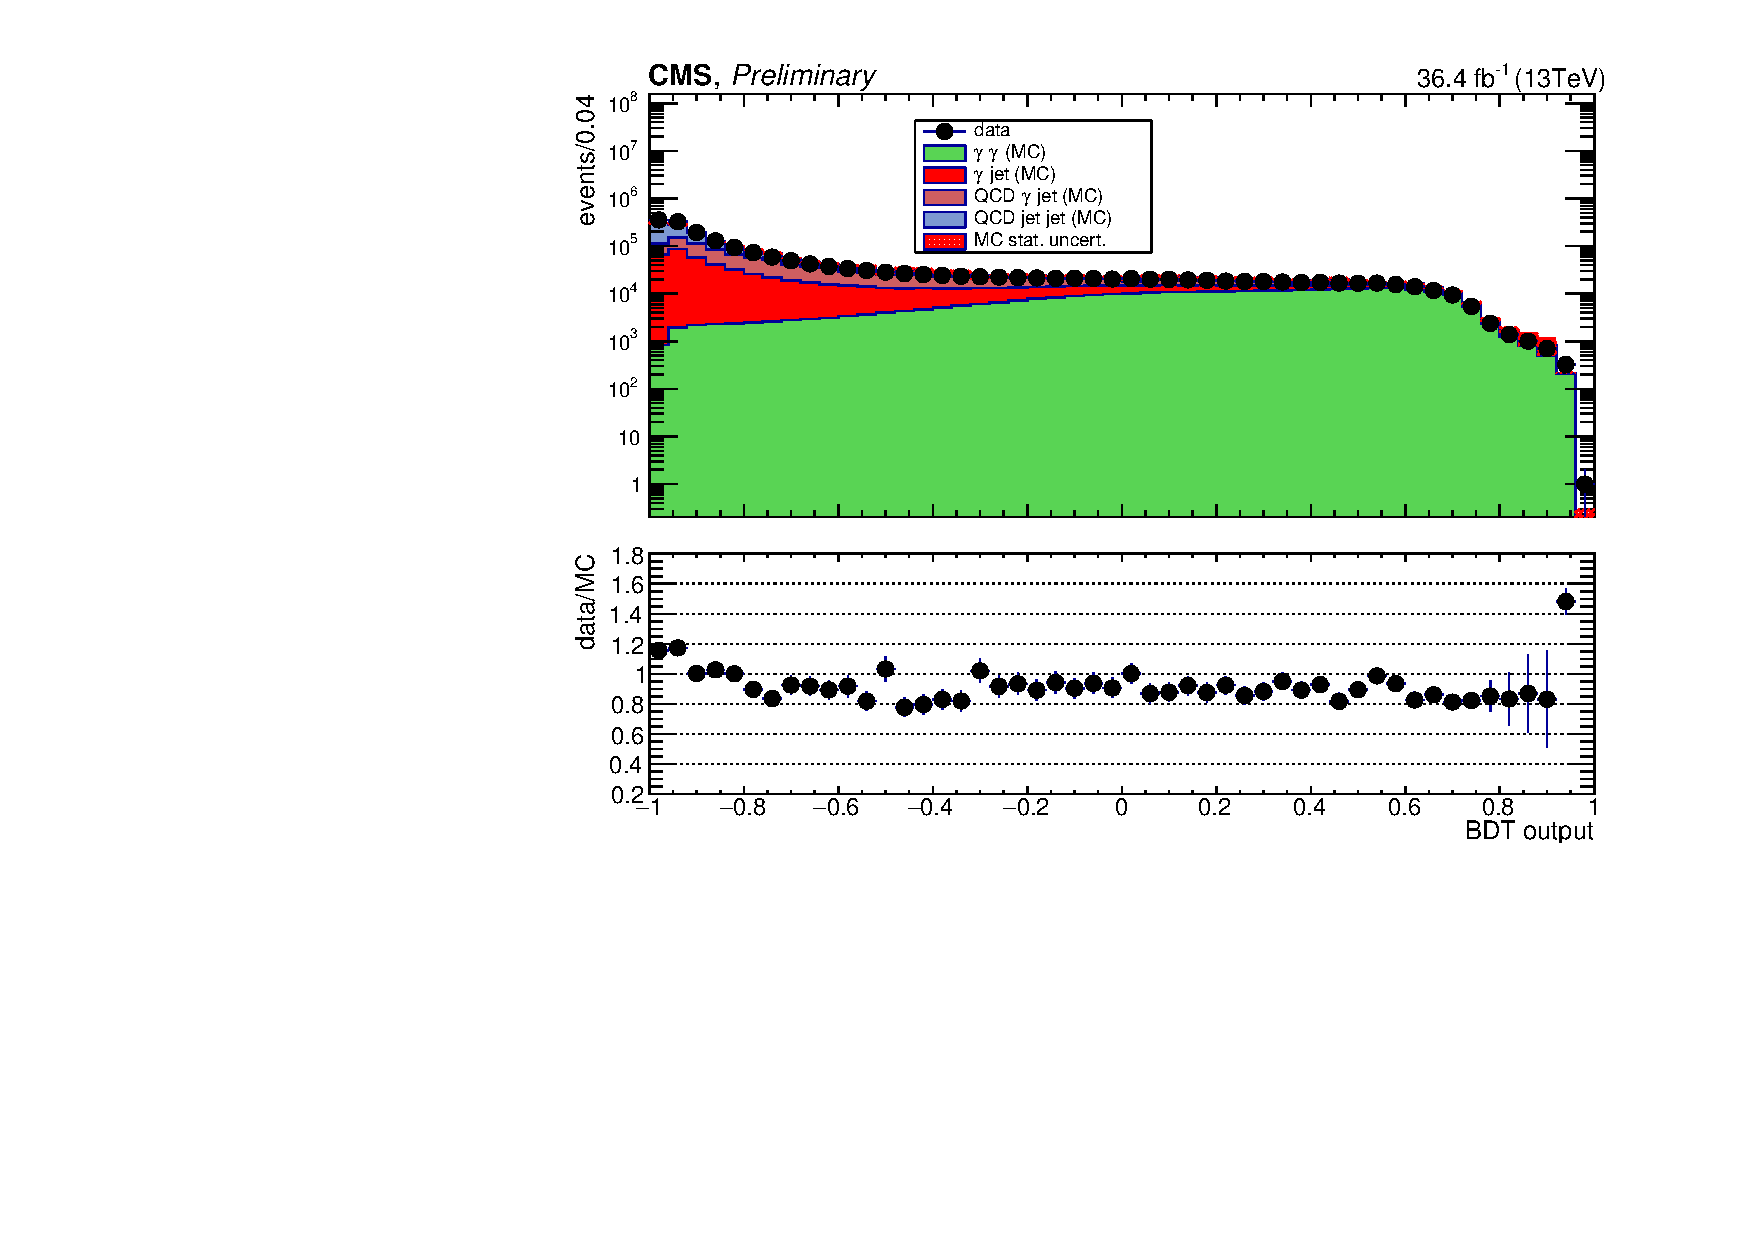
\includegraphics[width=0.5\textwidth]{catFigures/\whichFig/BDTgg.pdf}
\label{fig:cat:diphobdt_a}
}
\\
 \subfloat[]{
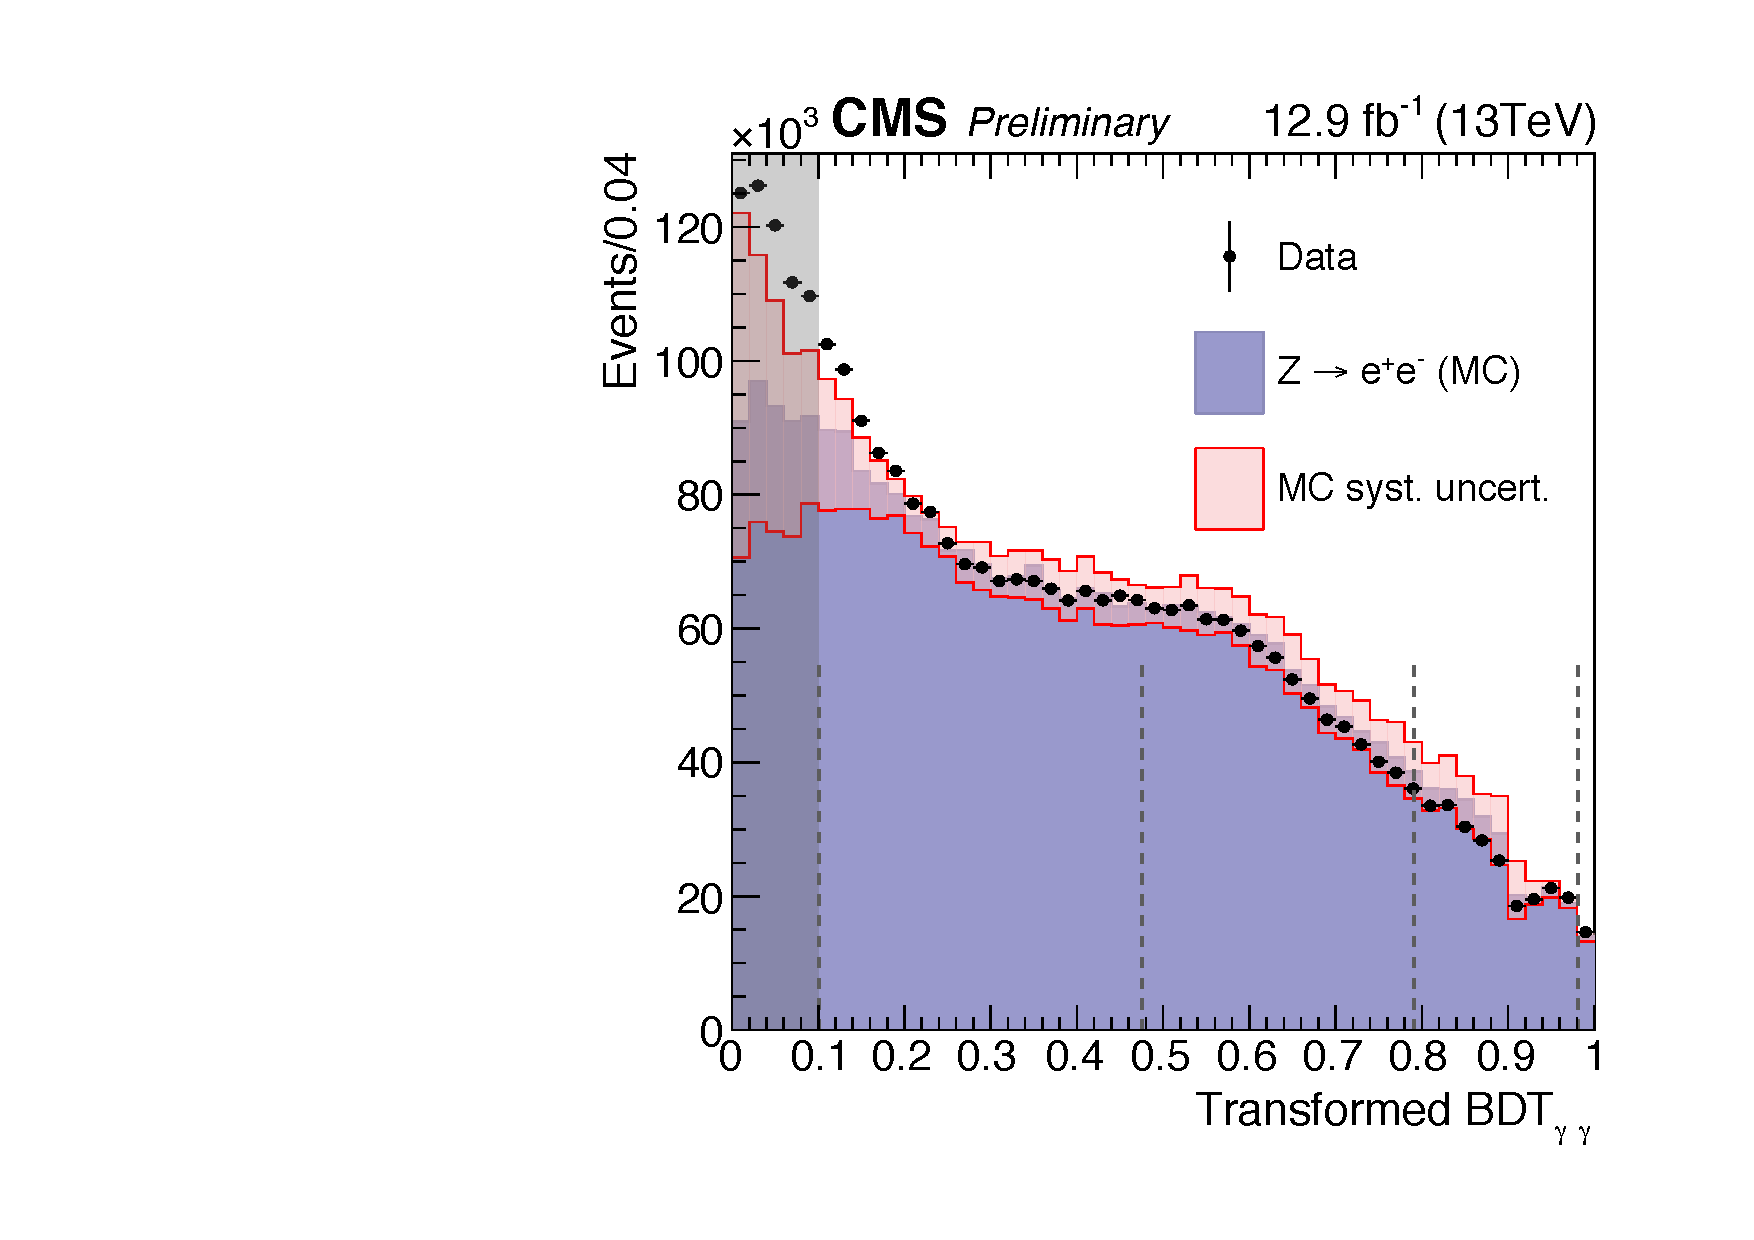
\includegraphics[width=0.5\textwidth]{catFigures/\whichFig/BDTgg_Zee.pdf}
\label{fig:cat:diphobdt_b}
}
\caption{ (a) The transformed \DiPhoBdt score for simulated signal and background events in the range $100 < \mgg < 180\GeV$. The transformation flattens the signal distribution. (b) The transformed \DiPhoBdt score for \Zee events in data and simulation, where the electrons are reconstructed as photons. The pink shading represents the systematic uncertainty associated with the \PhoIdBdt and the \PhoEnergyBdt. For both (a) and (b), the vertical dashed lines represent the boundaries of the Untagged categories described in \Sec~\ref{cat:sec:untagged}, while the grey shading represents the area for which diphotons are rejected.}
\label{fig:cat:diphobdt}
\end{figure}

\section{\VBFTag categories }
\label{cat:sec:vbftag}

%Higgs bosons in \CMS are produced chiefly via the \ggH production mode in the LHC environment. In this mode, the final state of the interaction involving the Higgs boson contains only the Higgs boson decay products to first order. Other production modes, by contrast, produce a Higgs boson in association with other particles. The additional particles can therefore be used to identify Higgs bososn events produced via \VBF, \VH or \ttH. 
The \VBF production mode has a cross-section approximately ten times smaller than that of the \ggH mode. The additional high-\pT jets in the event allow the identification of \VBF-like events with a high signal-to-background ratio. For this reason, although \VBF events occur much less frequently than \ggH events, defining \VBFTag categories significantly improves the overall sensitivity of the analysis.

Candidate \VBF events are selected by requiring that they contain two jets reconstructed as described in \Sec~\ref{reco:sec:jets} after \PFCHS with respect to the selected diphoton vertex. Furthermore, the jets must pass requirements aimed at removing jets that originate from other \pp interactions in the event, and must be separated from the leading and subleading photons by $\Delta R > 0.4$. The leading (subleading) jet is required to satisfy $\pT > 30 \GeV$ ($\pT > 20 \GeV$). For events passing these requirements, an additional selection on the invariant mass of the \emph{dijet} composed of the leading and subleading jets, \mjj, is imposed: $\mjj > 250\GeV$. %Events which satistfy all of the above are said to pass the \emph{dijet preselection}.

For events passing the dijet preselection described above, the \VBFTag categorisation proceeds as follows. First, a \BDT referred to as \DiJetBdt is trained to give a high score to events where the dijets are \VBF-like. In particular, this is trained to reject \ggH events, and so cannot directly incorporate information about the diphoton quality from the \DiPhoBdt. %The \DiJetBdt is trained to treat simulated \VBF events as signal, and to treat simulated \ggH events (where dijets are formed from \PU and initial or final state radiation) and \SM processes which produce jets as background. 
A further \BDT referred to as the \DiPhoDiJetBdt, which treats \ggH events as neither signal nor background, is used to include the expected signal-to-background ratio of the diphoton. The \DiPhoDiJetBdt has the \DiPhoBdt and the \DiJetBdt output scores as its inputs variables. It is thus able to combine the \VBF-like dijet identification power of one \BDT with with mass resolution information from the other. %In the \DiPhoDiJetBdt, \ggH events cannot be treated as background since the \DiPhoBdt would not be well-behaved. So \ggH events are treated as neither signal nor background when training the \DiPhoDiJetBdt. 
A selection on the output score of the \DiPhoDiJetBdt is then used to categorise the candidate \VBFTag events.

The \DiJetBdt is trained on simulated samples of diphoton events where the signal is defined as \VBF (\Hgg) events. The background consists of samples of \SM events with a diphoton and a dijet in the final state, in addition to a simulated sample of \ggH events where dijets are formed from \PU and initial or final state radiation. The input variables for this \BDT are listed below:
\begin{itemize}
\item the invariant-mass-scaled transverse momentum ($\pT/\mgg$) for the leading and subleading photons in the diphoton candidate;
\item the transverse momenta of the leading and subleading jets in the dijet;
\item \mjj;
\item $|\eta_{\text{j}_1} - \eta_{\text{j}_2}|$, the separation of the jets in the dijet in the $\eta$-direction;
\ifNewAnalysis
\item $C_{\gamma\gamma} = \exp(-\frac{4}{(\eta_{j_1}-\eta_{j_2})^2}(\eta_{\gamma\gamma}-\frac{\eta_{j_1}+\eta_{j_2}}{2}))$, the so-called centrality of the diphoton-dijet system;
\else
\item $\eta^{*} = |\eta_{\gamma\gamma} - (\eta_{j_1}+\eta_{j_2})/2|$, the \emph{Zeppenfeld} variable~\cite{Zeppenfeld};
\fi
\item $|\phi_{\gamma\gamma} - \phi_\text{jj}|$, the separation of the dijet and the diphoton in the $\phi$-direction.
\end{itemize}
%The \DiJetBdt output scores for each simulated signal sample are shown in \Fig~\ref{fig:cat:dijetbdt_sig}. 
The distributions of the \DiJetBdt output scores for data and simulated background samples (and some simulated signal samples) are shown in \Fig~\ref{fig:cat:dijetbdt_all}. 


The \DiPhoDiJetBdt is trained on simulated events where the signal is a sample of \VBF \Hgg events, while the background is composed of the \SM diphoton background samples, as for the \DiJetBdt training. In this case, the \ggH events are used neither as signal nor as background. The inputs to the \BDT are the following:
\begin{itemize}
\item the output score of the \DiPhoBdt;
\item the output score of the \DiJetBdt;
\item $\pT^{\gamma\gamma}/\mgg$, the invariant-mass-scaled momentum of the diphoton system, which is included since it has a significant correlation to both the other inputs.
\end{itemize}
%The distributions of the \DiPhoDiJetBdt output scores for each simulated signal sample are shown in \Fig~\ref{fig:cat:diphodijetbdt_sig}. 
The distributions of the \DiJetBdt output scores for data and simulated background samples are shown in \Fig~\ref{fig:cat:diphodijetbdt_all}. 

%\begin{figure}[h]
%\centering
 %\subfloat[\DiPhoDiJetBdt output by production mode.]{
%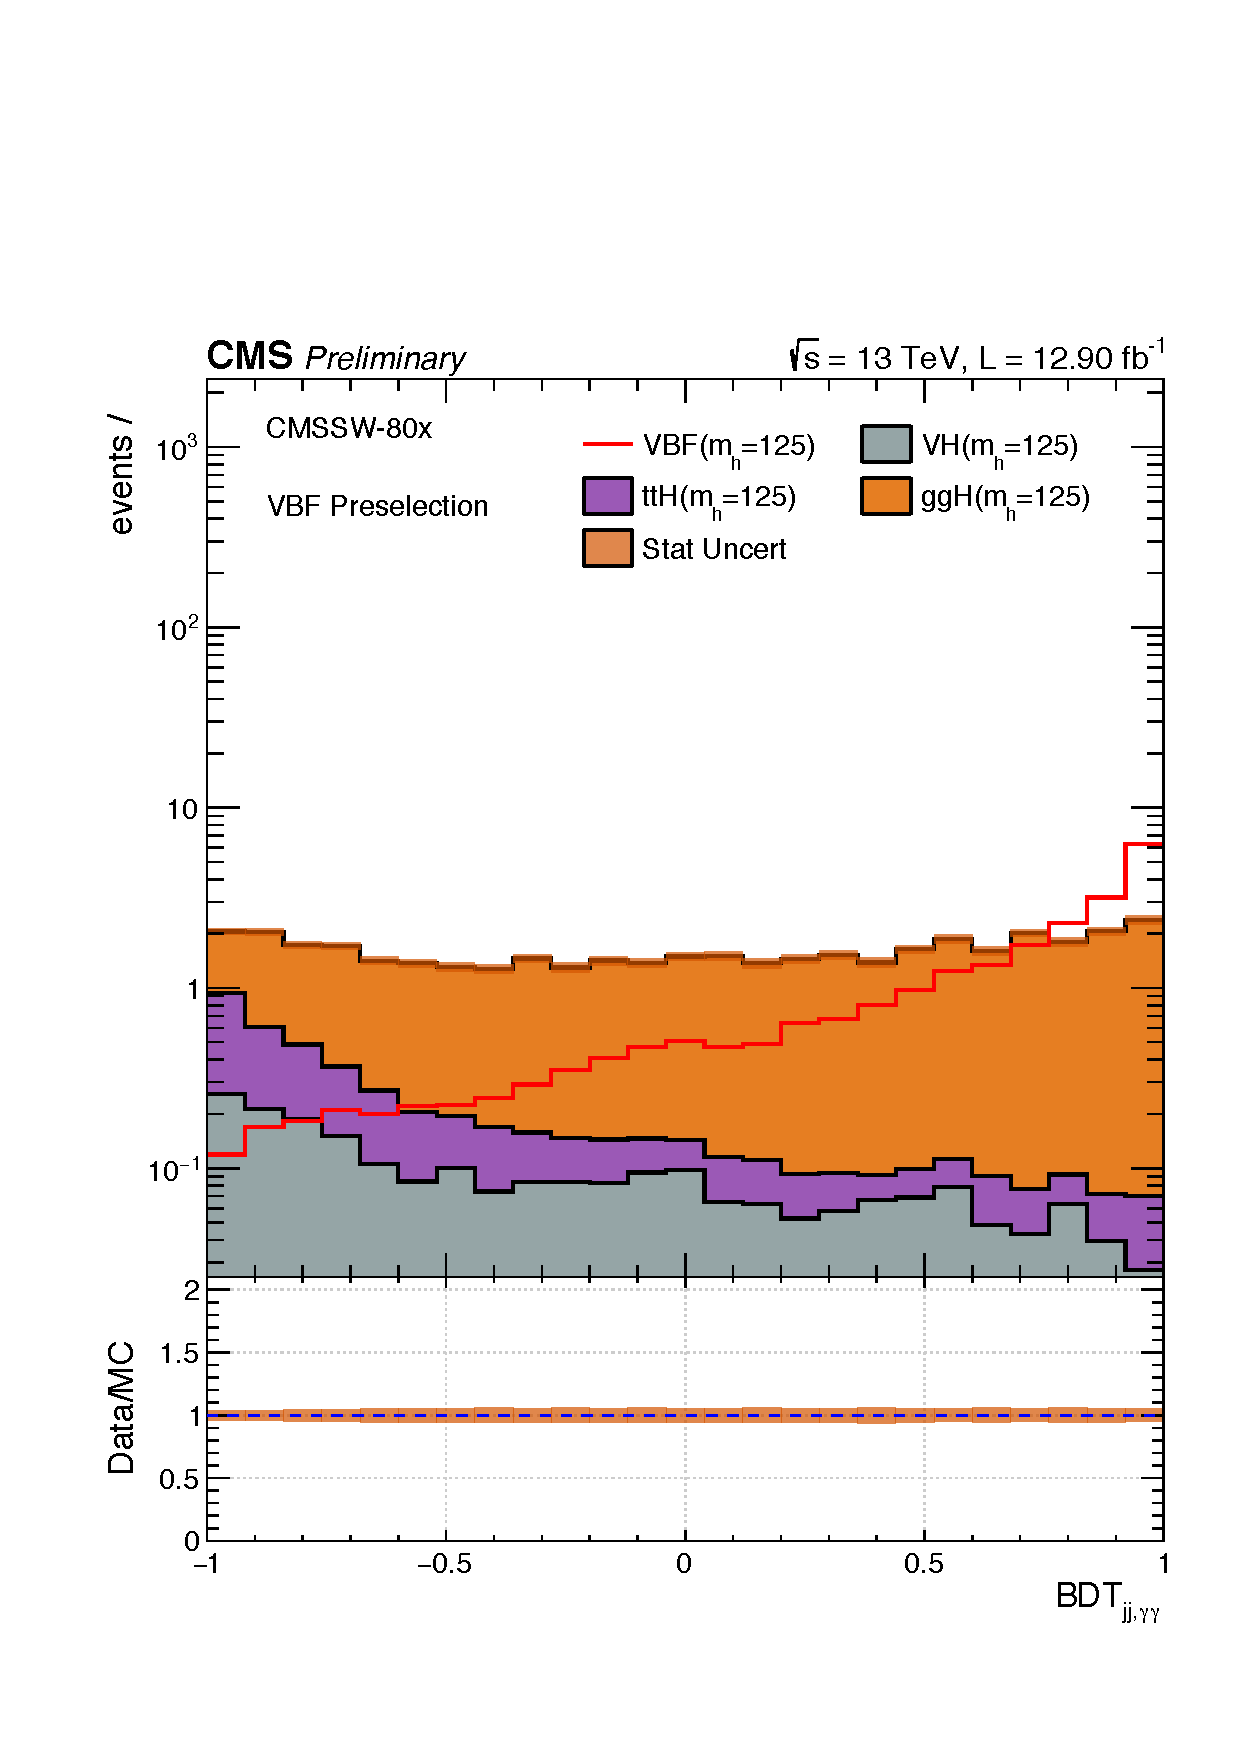
\includegraphics[width=0.45\textwidth]{catFigures/stack_histogram_dipho_dijet_MVA_signal_14-07-2016_.pdf}
%\label{fig:cat:diphodijetbdt_sig}
%}
%\caption{The output scores of the \DiJetBdt and \DiPhoDiJetBdt split by simulated production mode and comparing data and simulated signal and background.}
%\label{fig:cat:vbf_bdts}
%\end{figure}

\begin{figure}[tph]
\centering
% \subfloat[\DiJetBdt output by production mode.]{
%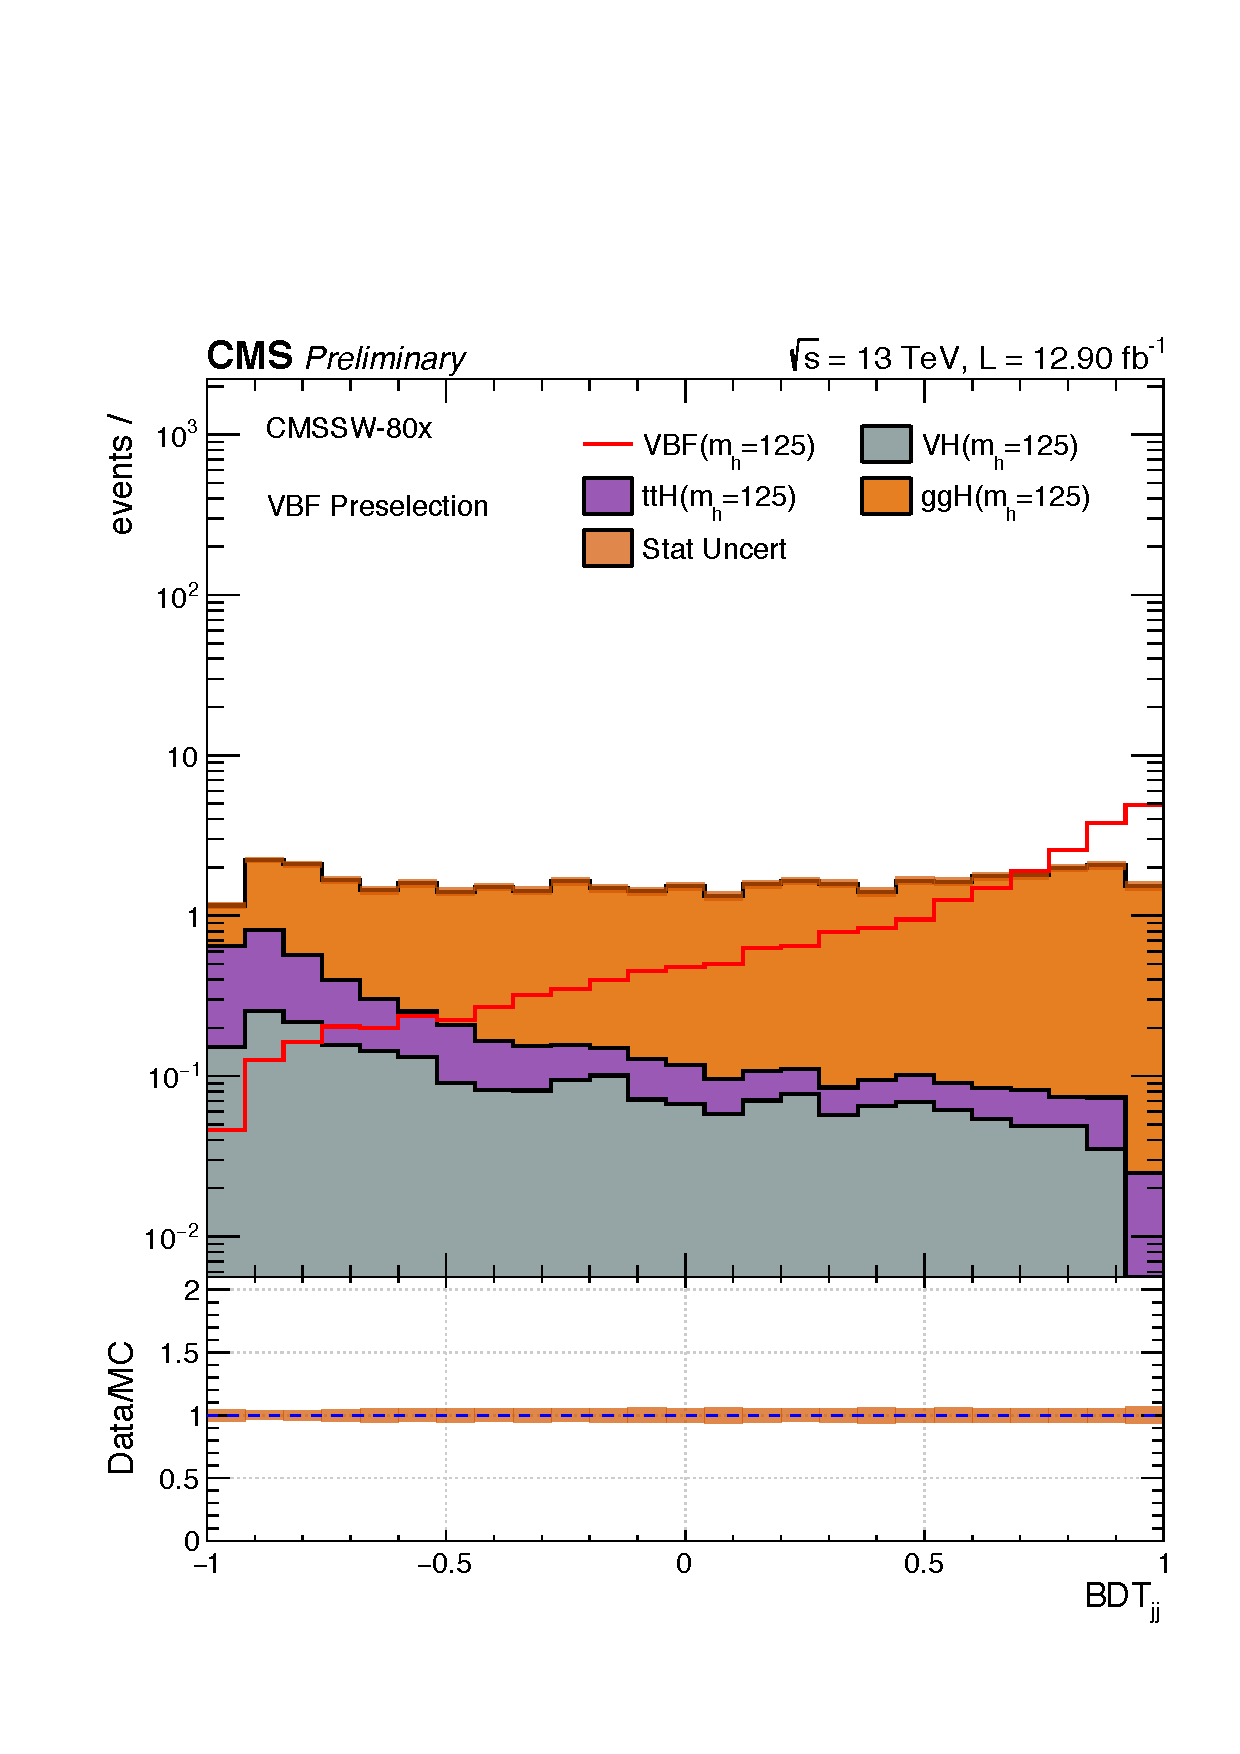
\includegraphics[width=0.45\textwidth]{catFigures/\whichFig/stack_histogram_dijet_mva_signal_14-07-2016_.pdf}
%\label{fig:cat:dijetbdt_sig}
%}
 \subfloat[\DiJetBdt output comparing data and simulated signal and background.]{
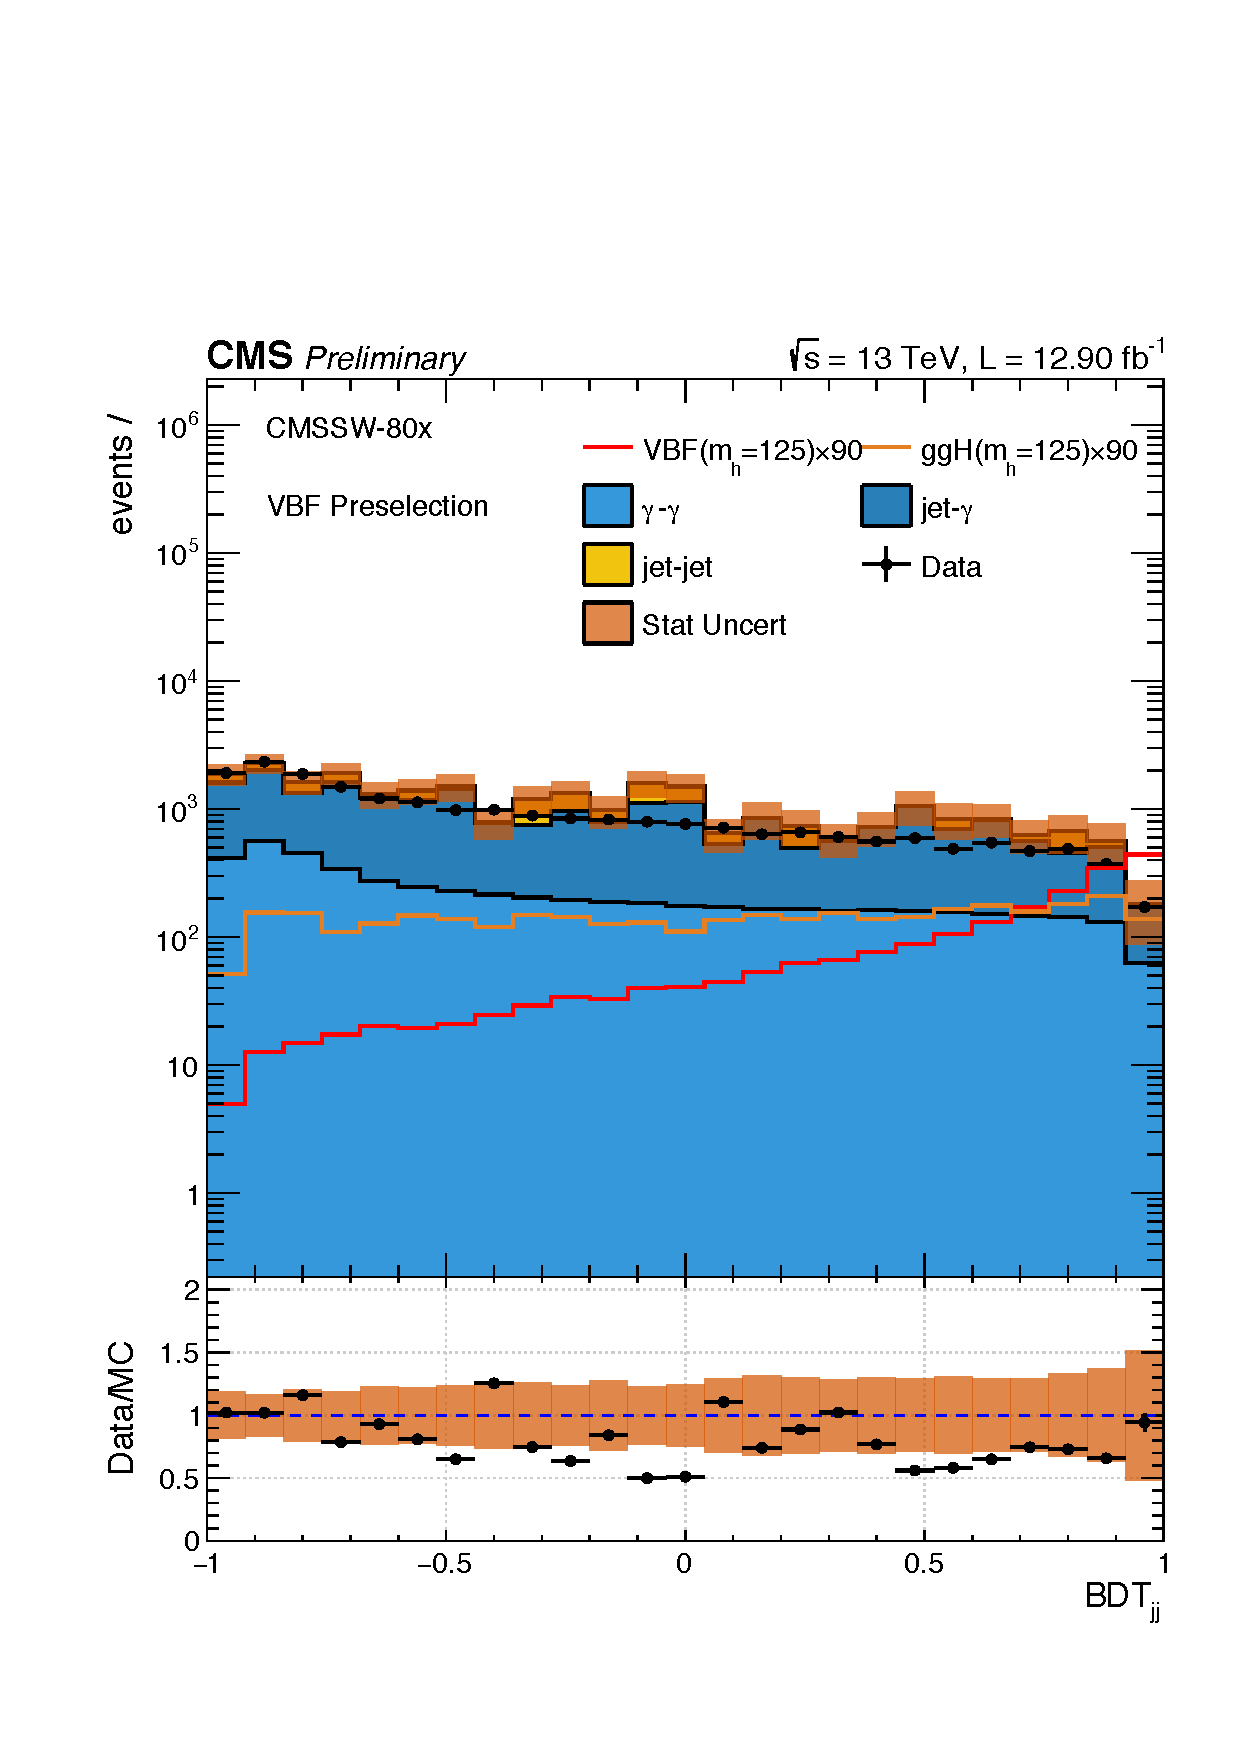
\includegraphics[width=0.5\textwidth]{catFigures/\whichFig/stack_histogram_dijet_mva.pdf}
\label{fig:cat:dijetbdt_all}} \\
 \subfloat[\DiPhoDiJetBdt output comparing data and simulated signal and background.]{
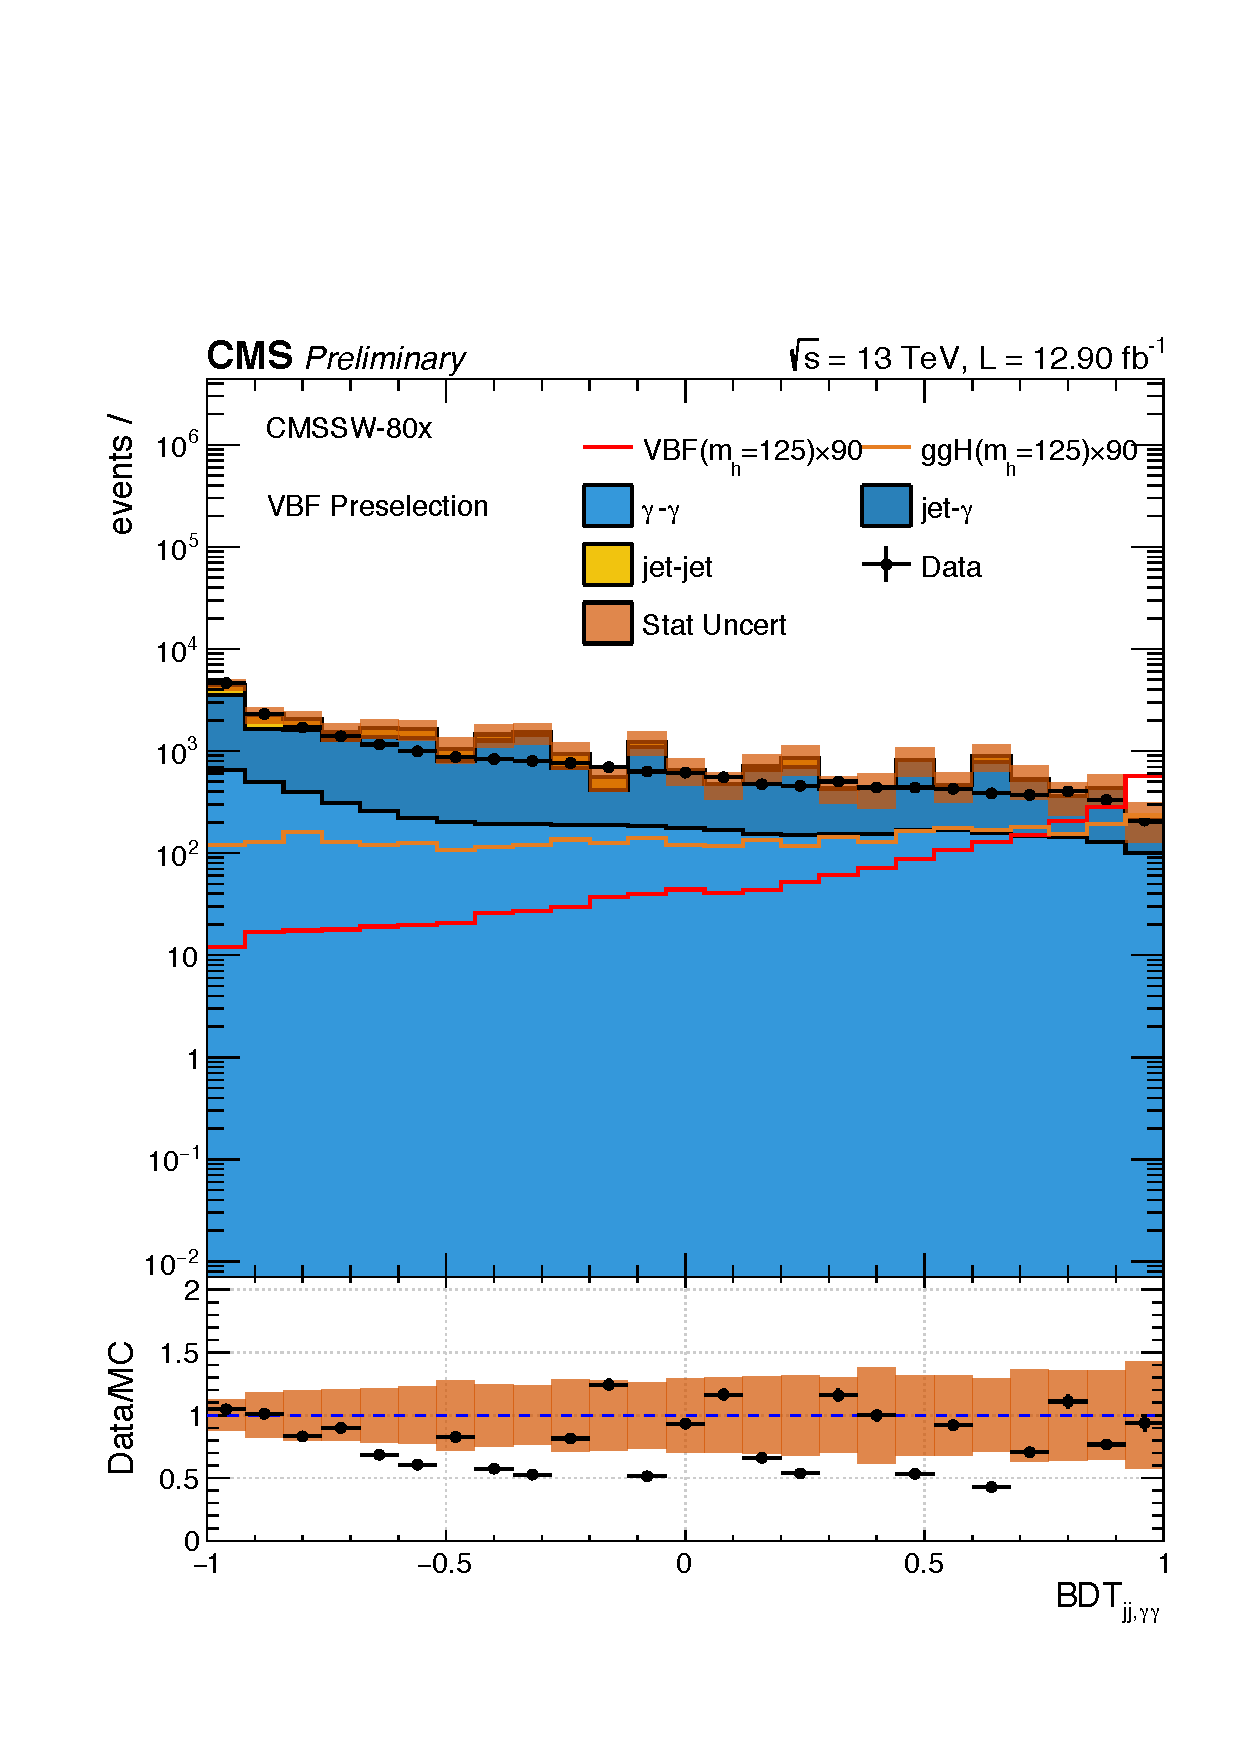
\includegraphics[width=0.5\textwidth]{catFigures/\whichFig/stack_histogram_dipho_dijet_mva.pdf}
\label{fig:cat:diphodijetbdt_all}}
\caption{The output scores of the \DiJetBdt (a) and \DiPhoDiJetBdt (b) split by simulated production mode and comparing data and simulation. The dijet preselection has been applied in both cases. }
\label{fig:cat:dijet_bdt}
\end{figure}

\ifNewAnalysis
Four \VBFTag categories (labelled 0, 1, 2, 3 from tightest to loosest) are defined by selections on the \DiPhoDiJetBdt output score. 
The location of the boundaries is optimised first by maximising the value of the signal-to-background ratio in the \VBFTag 0 category, and then repeating the procedure after fixing the first boundary to maximise the signal-to-background ratio in the \VBFTag 1 category, and so on. Of the simulated signal events in the \VBFTag categories, a non-negligible proportion originate from the \ggH process. The exact composition of the categories is shown in \Table~\ref{tab:model:sig_bkg_yields} in Chapter~\ref{chap:model}. Events for which the \DiPhoDiJetBdt output score is below the lowest boundary fail the \VBFTag categorisation, but may be still included in other analysis categories. Repeating the optimisation procedure for five \VBF-tagged categories did not lead to an improvement in the expected sensitivity of the analysis.
\else
Two \VBFTag categories (labelled 0 and 1) are defined by selections on the \DiPhoDiJetBdt output score. 
The location of the two boundaries is optimised first by maximising the value of the signal-to-background ratio in the \VBFTag 0 category, and then repeating the procedure after fixing the first boundary to maximise the signal-to-background ratio in the \VBFTag 1 category. Of the simulated signal events in the \VBFTag 0 category, approximately 72\% are \VBF events and 27\% are \ggH events. The corresponding values for the \VBFTag 1 category are 55\% for \VBF events and 43\% for \ggH events. Events for which the \DiPhoDiJetBdt output score is below the lowest boundary fail the \VBFTag categorisation, but may be still included in other analysis categories. Repeating the optimisation procedure for three \VBF-tagged categories did not lead to an improvement in the expected sensitivity of the analysis.
\fi

\ifNewAnalysis
\section{\VHTag categories}
\label{cat:sec:vhtag}

Higgs boson events resulting from \VH production can be selected using the decay products of the $\PW$ or $\PZ$. The vector bosons can decay leptonically via $\PW \rightarrow \Plepton \Pneutrino$ or $\PZ \rightarrow \Plepton^{+} \Plepton^{-}$, or they can decay to quarks which hadronize to form jets. Finally, the $\PZ$ can decay to a pair of neutrinos, which are reconstructed as a large amount of missing energy. In this analysis, five categories are defined to exploit these final states, and their selections are defined in this section. %Although the addition of the \VHTag categories does not appreciably improve the overall sensitivity of the analysis, it allows the measurement of the cross-section of the \VH production mode. 
%For all \VHTag categories, events must pass the preselection defined in \Sec~\ref{reco:sec:pho:preselection}. 

The \VHLeptonicTag categories target events with at least one high-\pT charged lepton. Signal events which enter these categories are most often \WH events, which have a larger rate than \ZH when \crosssection and branching fraction to leptons are taken into account. The majority of signal events therefore contain a single high-\pT lepton and large \MET from the neutrino. Such events are targeted by the \WHLeptonicTag category. Conversely, the reconstructible \ZH events contain two leptons, which allows such events to be selected with a good signal-to-background ratio by the \ZHLeptonicTag category. A less sensitive \VHLeptonicLooseTag category is also defined, the purpose of which is to select events from \WH or \ZH where one of the leptons or the magnitude of the \MET was mis-reconstructed. 
%The \pT spectrum of Higgs decay particles is shifted towards higher values for \VH events than for \ggH events (due to recoil against the vector boson), and therefore the leading photon \pT requirement is increased, with the value the selection depending on the category.% to $\pT/\mgg >1/2$ for all \VHTag categories. 

All \VHLeptonicTag categories have some common elements in their selection:
\begin{itemize}
\item the leading photon must satisfy an increased requirement $\pT/\mgg > 3/8$, since the \pT spectrum of Higgs decay particles is shifted towards higher values for \VH events than for \ggH events (due to recoil against the vector boson);
\item the diphoton mass pass a loose requirement on its \DiPhoBdt output score; %, which keeps X\% of the signal while rejecting Y\% of the background events;
\item in \DY events, one or both electrons are sometimes incorrectly reconstructed as photons. Furthermore, prompt photons can be produced from initial or final state radiation. Therefore, an electron-photon system can mimic a diphoton, with the additional electron faking a \VH event. All electron tracks are therefore required to be $\Delta R > 0.4$ away from candidate photons;
\item similarly, \Zg events (where \Zee) can mimic \VH events if one of the electron tracks is not reconstructed. The invariant mass of both possible electron-photon systems must therefore be more than 10\GeV away from the mass of the $\PZ$ boson;
%\item electrons and muons used for the selections must satisfy a set of identification requirements, and must be separated from the photon candidates by at least $\Delta R > 0.5$ for muons and $\Delta R > 1.0$ for electrons.
\item muons used for the selection must be within $|\eta|<2.4$, pass a selection based on the properties of their tracks in the tracker and muon chambers and satisfy requirements on their \PU-corrected isolation. Electrons used for the selection must pass loose identification requirements;
\item there must be two or fewer jets with $\pT>20\GeV$, $|\eta|<2.4$ and within $\Delta R <0.4$ of the photons or leptons in the event, to avoid selecting events from the \ttH process. 
\end{itemize}

In addition to the common selection, events entering the \WHLeptonicTag category must contain at least one reconstructed electron or muon with $\pT > 20\GeV$ and contain at least $45\GeV$ of \MET. The \ZHLeptonicTag category requires two leptons of the same flavour in the event, both with $\pT>20\GeV$. The invariant mass of these two leptons must be in the range of $70$ to $110$\GeV. Finally, the \VHLeptonicLooseTag category has similar requirements to the \WHLeptonicTag category, but the selection on the \MET is inverted.

The \VHMetTag category targets events where: either the lepton from $\PW$ is outside of detector acceptance or otherwise not reconstructed; or the $\PZ$ decays to two neutrinos, and thus leaves no energy in the detector. This results in a large amount of reconstructed \MET in addition to the high-\pT photons from the Higgs boson decay. Events selected by the \VHMetTag category must satisfy the following requirements:
\begin{itemize}
\item the leading photon must satisfy an increased requirement $\pT/\mgg > 3/8$;
\item the diphoton mass pass a loose requirement on its \DiPhoBdt output score; % which keeps X\% of the signal while rejecting Y\% of the background events;
\item the event must contain $\MET > 70\GeV$;
\item the \MET direction and the momentum of the diphoton system must be separated in the $\phi$-direction by at least 2.1 radians, since they are expected to be back-to-back due to momentum conservation.
\end{itemize}

Finally, the \VHHadronicTag category targets events where the vector boson decays to quarks, leading to two jets in the event. 
The following selections are used for this category:
\begin{itemize}
\item the leading photon must satisfy an increased requirement $\pT/\mgg > 1/2$;
\item the event must contain at least two jets with $\pT>40\GeV$ and $|\eta|<2.4$, which must be $\Delta R >0.4$ away from the photons or leptons ;
\item the invariant mass of the dijet system must be in the range $[60,120]\GeV$;
\item the angle $\theta^{*}$ between the diphoton direction in the diphoton-dijet rest frame and the detector frame must satisfy $|\cos{\theta^{*}}| <0.5$ to exploit differences in the angular correlation of the diphoton and the dijet for \VH events.
\end{itemize}

Events which fail the selections for the \VHTag categories may still be selected for other categories.
\fi


\section{\TTHTag categories}
\label{cat:sec:tthtag}

Events where a Higgs boson is produced in association with a pair of top quarks will contain a pair of $\Pbottom$ quarks and $\PW$ bosons from their decay. The $\PW$ bosons will then decay either hadronically or leptonically. The cross-section of \ttH production is low, so the benefit to the analysis in terms of final significance of an observation is small. However, the categorisation of \ttH-like events is important because it allows an estimate of the strength of the interaction of the Higgs boson with top quarks. Various extensions to the \SM predict enhanced values of the strength of the \ttH interaction, and such models can be tested through the experimental measurement of the cross-section of \ttH events decaying to \Hgg.

Two exclusive \TTHTag categories are defined in this analysis. On the one hand, the \TTHLeptonicTag category aims to select \ttH events where at least one of the $\PW$ bosons decayed leptonically. On the other hand, the \TTHHadronicTag category targets events where both $\PW$ bosons decayed to quarks. In addition to the usual preselection applied to candidate events, the requirement on the leading photon \pT is increased to $\pT>\mgg/2$, because the \pT spectrum of Higgs decay particles is shifted towards higher values due to recoil against the $\Ptop \Ptop$ system. %for the same reason as described in \Sec~\ref{cat:sec:vhtag}. %The selections for each of these categories are defined separately and are described below.

The leptons which are used in the selection must pass the same identification requirements as those uised for the \VHLeptonicTag categories. In order to be included in the \TTHLeptonicTag category, events must satisfy the following conditions:
\begin{itemize}
\item the diphoton must satisfy a loose selection on the \DiPhoBdt output which has approximately 70\% signal selection efficiency and 15\% background selection efficiency; 
\item the event must contain at least one selected lepton with $\pT>20\GeV$; %If the lepton is an electron,n;%$Muons are required to be within $|\eta|<2.4$, pass a selection based on the properties of the tracks it leaves in the tracker and muon chambers and satisfy a requirement on its \PU-corrected charged hadron, neutral hadron and photon isolations (with cone size $R=0.4$). Electrons are required to be within the \ECAL
\item the event must contain at least 2 jets with $\pT>25\GeV$, $|\eta|<2.4$ and separated by at least a distance $\Delta R=0.4$ from a photon or lepton candidate;
\item at least one of the jets should be tagged as a $\Pbottom$ jet using the CVSv2 algorithm medium requirement, as described in~\cite{bjets}.
\end{itemize}

For events to be included in the \TTHHadronicTag category, the following selections are made:
\begin{itemize}
\item the diphoton must satisfy a loose selection on the \DiPhoBdt output score which has approximately 95\% signal selection efficiency and 45\% background selection efficiency; 
\item there must be no leptons in the event which meet the requirements for the \TTHLeptonicTag category;
\item there must be at least five jets in the event satisfying $\pT >25\GeV$;
\item at least one of the jets should be tagged as a $\Pbottom$ jet using the CVSv2 algorithm medium requirement, as described in~\cite{bjets}.
\end{itemize}

Events which fail the selections for the \TTHTag\s may still be selected for other categories.

\section{Inclusive categories}
\label{cat:sec:untagged}

The remaining events are split into inclusive categories using the \DiPhoBdt output score. The number of inclusive categories and the locations of the boundaries between them is optimised using simulated samples which are independent from those used to train the \DiPhoBdt. 

For a given number of inclusive categories $N_\text{cat}$, the boundaries are initially spaced evenly throughout the \DiPhoBdt output score distribution. Events falling below the lowest boundary are discarded. Simplified models are used to parametrise the signal and background \mgg distributions in the remaining categories. For the signal, a sum of two Gaussians is used, representing the detector resolution and the uncertainty due to incorrect vertex assignment respectively. The background \mgg spectrum is parametrised using an exponential. The expected significance is then obtained by producing and fitting an Asimov dataset~\cite{Cowan:2010js} in each category. The estimation of the expected significance is iteratively repeated, allowing the boundaries to float. The final set of boundaries is chosen such that the expected significance is maximised for a given $N_\text{cat}$.

The procedure can be repeated for different values of $N_\text{cat}$. In this analysis, $N_\text{cat}=4$ was chosen, as moving to $N_\text{cat}=5$ produced a negligible improvement in the expected significance. The boundaries are represented by the vertical dashed lines in \Fig\s~\ref{fig:cat:diphobdt_a} and~\ref{fig:cat:diphobdt_b}. The resulting categories (labelled \Untagged) are numbered from 0 (highest signal-to-background ratio) to 3 (lowest signal-to-background ratio).

\section{Categorisation hierarchy}
\label{cat:sec:hierarchy}

Each event is tested to see if it can be included in the categories described previously, according to a hierarchy. If it satisfies the requirements of the first category, the event is assigned and the next event is tested. If not, the event is tested for next category in the hierarchy, and so on, until no further categories remain and the event is discarded. Each event is assigned to only one category in the hierarchy, which is ordered as follows: 
\ifNewAnalysis
\TTHLeptonicTag, \WHLeptonicTag, \ZHLeptonicTag, \VHLeptonicLooseTag, \VHMetTag, \TTHHadronicTag, \VHHadronicTag, \VBFTag 0, \VBFTag 1, \VBFTag 2, \VBFTag 3, \Untagged 0, \Untagged 1, \Untagged 2, \Untagged 3.
\else
\TTHLeptonicTag, \TTHHadronicTag, \VHHadronicTag, \VBFTag 0, \VBFTag 1, \Untagged 0, \Untagged 1, \Untagged 2, \Untagged 3.
\fi

  \chapter{Statistical analysis and results}
\label{chap:statandresults}

\ifNewAnalysis
The signal and background models described in \Chapter~\ref{chap:model} are used to perform the statistical interpretation of the \thisanalysislumi\ifb of data. The result is an independent observation of the Higgs boson in the diphoton decay channel and measurements of some of its properties. %The objective is to twofold:
\else
The signal and background models described in \Chapter~\ref{chap:model} are used to perform the statistical interpretation of \thisanalysislumi\ifb of \RunII data collected at $\sqrt{s}=13\TeV$ by \CMS in 2016. The author was responsible for the signal and background modelling, systematics handling and statistical interpretation in the official \CMS preliminary result~\cite{CMS-PAS-HIG-16-020} produced with the same dataset. The results presented in this section differ from those presented in~\cite{CMS-PAS-HIG-16-020} insofar as they use improvements to the signal modelling techniques developed by the author. Namely the \DCBpG functional form was used instead of a sum of Gaussians, and interpolation using \SSF was used instead of linear interpolation. The results from this thesis and~\cite{CMS-PAS-HIG-16-020} are almost identical, as expected, and are compared at various points throughout this chapter.

Due to the scaling of the \SM Higgs boson and background \crosssection\s moving from 7 or 8\TeV to 13\TeV, the dataset used in this thesis has roughly the same statistical sensitivity as the full \RunI dataset, which had an integrated luminosity of $24.8\ifb$. The final analysis of the \RunI dataset~\cite{LegacyHgg} led to an independent observation of the Higgs boson in the diphoton decay channel. The objective of the work presented in this thesis is therefore to make a confirmation of the observation (or ``rediscovery'') of the Higgs boson in the diphoton decay channel, and measurements of some of its properties.
\fi

The statistical analysis proceeds in several stages. The first step is to determine the best signal-plus-background fit of the models to the data. The floating parameters of the signal and background models are varied simultaneously in each analysis category to obtain the closest overall agreement with the observed invariant mass distributions. This procedure is described in \Sec~\ref{sec:statandresults:bestfit}, and leads to a Higgs boson signal being measured in the data. The next step is to quantify the significance of this signal and formally reject the hypothesis that there is no Higgs boson. The procedure for hypothesis testing and calculation of the significance is detailed in \Sec~\ref{sec:statandresults:significance}. Having established the existence of a \SM-like Higgs boson which decays to photons, the final step is to make measurements of some of its properties, in particular those which relate to the rate at which it is produced or interacts with other \SM particles. These measurements are described in \Sec~\ref{sec:statandresults:sigstrength} and \Sec~\ref{sec:statandresults:kappas}. 
 
As with all Higgs boson analyses performed within the \CMS collaboration, the statistical interpretation uses the frequentist approach. The corresponding statistical tools and techniques are briefly explained as they are needed throughout this chapter.

\section{Best fit of models to the data}
\label{sec:statandresults:bestfit}

The observed \mgg distributions obtained from the data (labelled $ \mgg^{obs}$ hereafter) are parametrised with models consisting of signal and background components. The tool which is used determine the model parameters and to assess the agreement with the data in a category $C$ is called the \emph{likelihood function},
\begin{equation}
\label{eq:statandresults:likelihood_function}
\mathcal{L}_C(\mu, \mH; \mathbf{n} | \mgg^{obs,C} ) = \mu \cdot f^C_S(\mgg^{obs,C} |\mH ; \mathbf{n}_S) + f^C_B(\mgg^{obs,C} | \mathbf{n}_B ). 
\end{equation}
In the definition above:
\begin{itemize}
\item $\mu = \sigma^{H} / \sigma^{H}_{SM}$ is a \POI called the signal strength, where in this context $\sigma^H$ is the observed Higgs boson cross section, and $\sigma^H_{SM}$ is the \SM Higgs boson \crosssection. The mass of the Higgs boson \mH is a second \POI. The likelihood function can in fact be generalised for an arbitrary number of \POI\s (as in \Sec\s~\ref{sec:statandresults:sigstrength} and~\ref{sec:statandresults:kappas}); 
\item $\mathbf{n}$ is a set of floating nuisance parameters, composed of those which affect the signal model and those which affect the background model, labelled $\mathbf{n}_S$ and $\mathbf{n}_B$ respectively;
\item $\mgg^{obs,C}$ is the invariant mass distribution for a particular category $C$;
\item $f^C_S$ and $f^C_B$ represent the probability distribution functions of the signal and background components of the model in category $C$, normalised to the expected number of signal and background events in that category respectively. Some of the nuisances parameters can modify the normalisation of $f^C_S$ and $f^C_B$. 
\end{itemize}

The construction of the signal component of the model in each category, $f^C_S$, was described in \Sec~\ref{model:sec:signal_model}, and is comprised of the individual models for each Higgs boson production process, each normalised to their respective expected number of events:
\begin{equation}
\label{eq:statandresults:f_s_breakdown}
\begin{split}
 f^C_S(\mgg^{obs,C} |\mH ; \mathbf{n}_S) ={} & f^C_{S,{\text{ggH}}}(\mgg^{obs,C} |\mH ; \mathbf{n}_S)  + f^C_{S,{\text{VBF}}}(\mgg^{obs,C} |\mH ; \mathbf{n}_S)\\
  & + f^C_{S,{\text{VH}}}(\mgg^{obs,C} |\mH ; \mathbf{n}_S)+ f^C_{S,{\text{ttH}}}(\mgg^{obs,C} |\mH ; \mathbf{n}_S).\\
\end{split}
\end{equation}

When performing the signal-plus-background fit to the data, the values of the individual parameters of the signal model functional form are fixed. Specifically, since the \SSF method was used, this refers to the coefficients of the seventeen polynomial functions which describe the dependence on \mH of the \DCBpG parameters for both the \RV and \WV scenarios and their mixing fraction. The parameters which are allowed to vary are the nuisance parameters $\mathbf{n}_S$ introduced into the signal modelling to account for systematic uncertainties (see \Sec~\ref{model:sec:systematics}), as well as the \POI\s $\mu$ and \mH. The signal strength $\mu$ uniformly scales all the signal models for each process and for each category. This means that the contribution to the overall signal model from each process remains in proportion to what is predicted by the \SM, but the normalisation of the overall signal model can be varied.

The handling of the background component of the model $f^C_B$, for a given category, was described in \Sec~\ref{model:sec:background_model}. The nuisance parameters $\mathbf{n}_B$ affecting the background model are composed of:
\begin{itemize}
\item the discrete nuisance parameter in each category which corresponds to the choice of background function, as prescribed by the discrete profiling method (see \Sec~\ref{model:sec:background_model_envelope}); 
\item the individual parameters of all the candidate functions, in all categories, which are allowed to float in the fit.
\end{itemize}

The overall likelihood function $\mathcal{L}$ for the simultaneous fit of all categories at once is obtained by taking the product of the likelihood functions $\mathcal{L}_C$ in each analysis category, taking care to correlate the corresponding nuisance parameters in each one:
\begin{equation}
\label{eq:statandresults:likelihood_function_product}
\mathcal{L}(\mu, \mH; \mathbf{n} | \mgg^{obs} ) = \prod_{C} \mathcal{L}_C(\mu, \mH; \mathbf{n} | \mgg^{obs,C} ).
\end{equation}

%The fit is obtained by minimising twice the negative log-likelihood ($ -2 \ln \mathcal{L}(\mu, \mH ; \mathbf{n}| \mgg^{obs}$) or \NLL). 
The fit is obtained by minimising twice the negative log-likelihood (\NLL). 
The best-fit values of the \POI\s and nuisance parameters are denoted as $\hat{\mu}$, $\hat{\mH}$ and $\hat{\mathbf{n}}$, such that:
\begin{equation}
%(\hat{\mu}, \hat{\mH} , \hat{\mathbf{n}}) = 
\{ (\mu, \mH, \mathbf{n}) : -2 \ln \mathcal{L}(\hat{\mu}, \hat{\mH} ;\hat{\mathbf{n}}| \mgg^{obs}) = \min _{\mu,\mH , \mathbf{n}}(-2 \ln \mathcal{L}(\mu, \mH; \mathbf{n}| \mgg^{obs})) \},
\end{equation}
where $\displaystyle\min_{ \mu, \mH ,\mathbf{n}}$ represents the global minimum evaluated over all allowed values of $\mu$, \mH and $\mathbf{n}$, taking into account their constraints. The parameters in this analysis are constrainted in one of three possible ways: for the systematic uncertainties described by shape nuisances, a Gaussian constraint is applied ; for the systematic uncertainties described by yield or migration nuisances, a log-normal constrain is applied ; for all other nuisances, the constraint is flat. 

 In general, the \NLL cannot be minimized analytically. Instead, this task is handled numerically with the \Minuit minimizer~\cite{minuit}, as part of the \RooFit software package~\cite{RooFit}. 
The resulting parametrisations of the observed data are shown for each analysis category separately in \Fig\s~\ref{fig:statandresults:s_b_fits} and~\ref{fig:statandresults:s_b_fits_bis}. The combined parametrisation and data resulting from a direct sum of each category is shown in \Fig~\ref{fig:statandresults:s_b_fits_direct_sum}, while the sum weighted by the $S/(S+B)$ in $\pm \effSigma$ around the best-fit $\mH$ in each category is shown in \Fig~\ref{fig:statandresults:s_b_fits_s_sb_sum}. 

\begin{figure}[p]
\centering
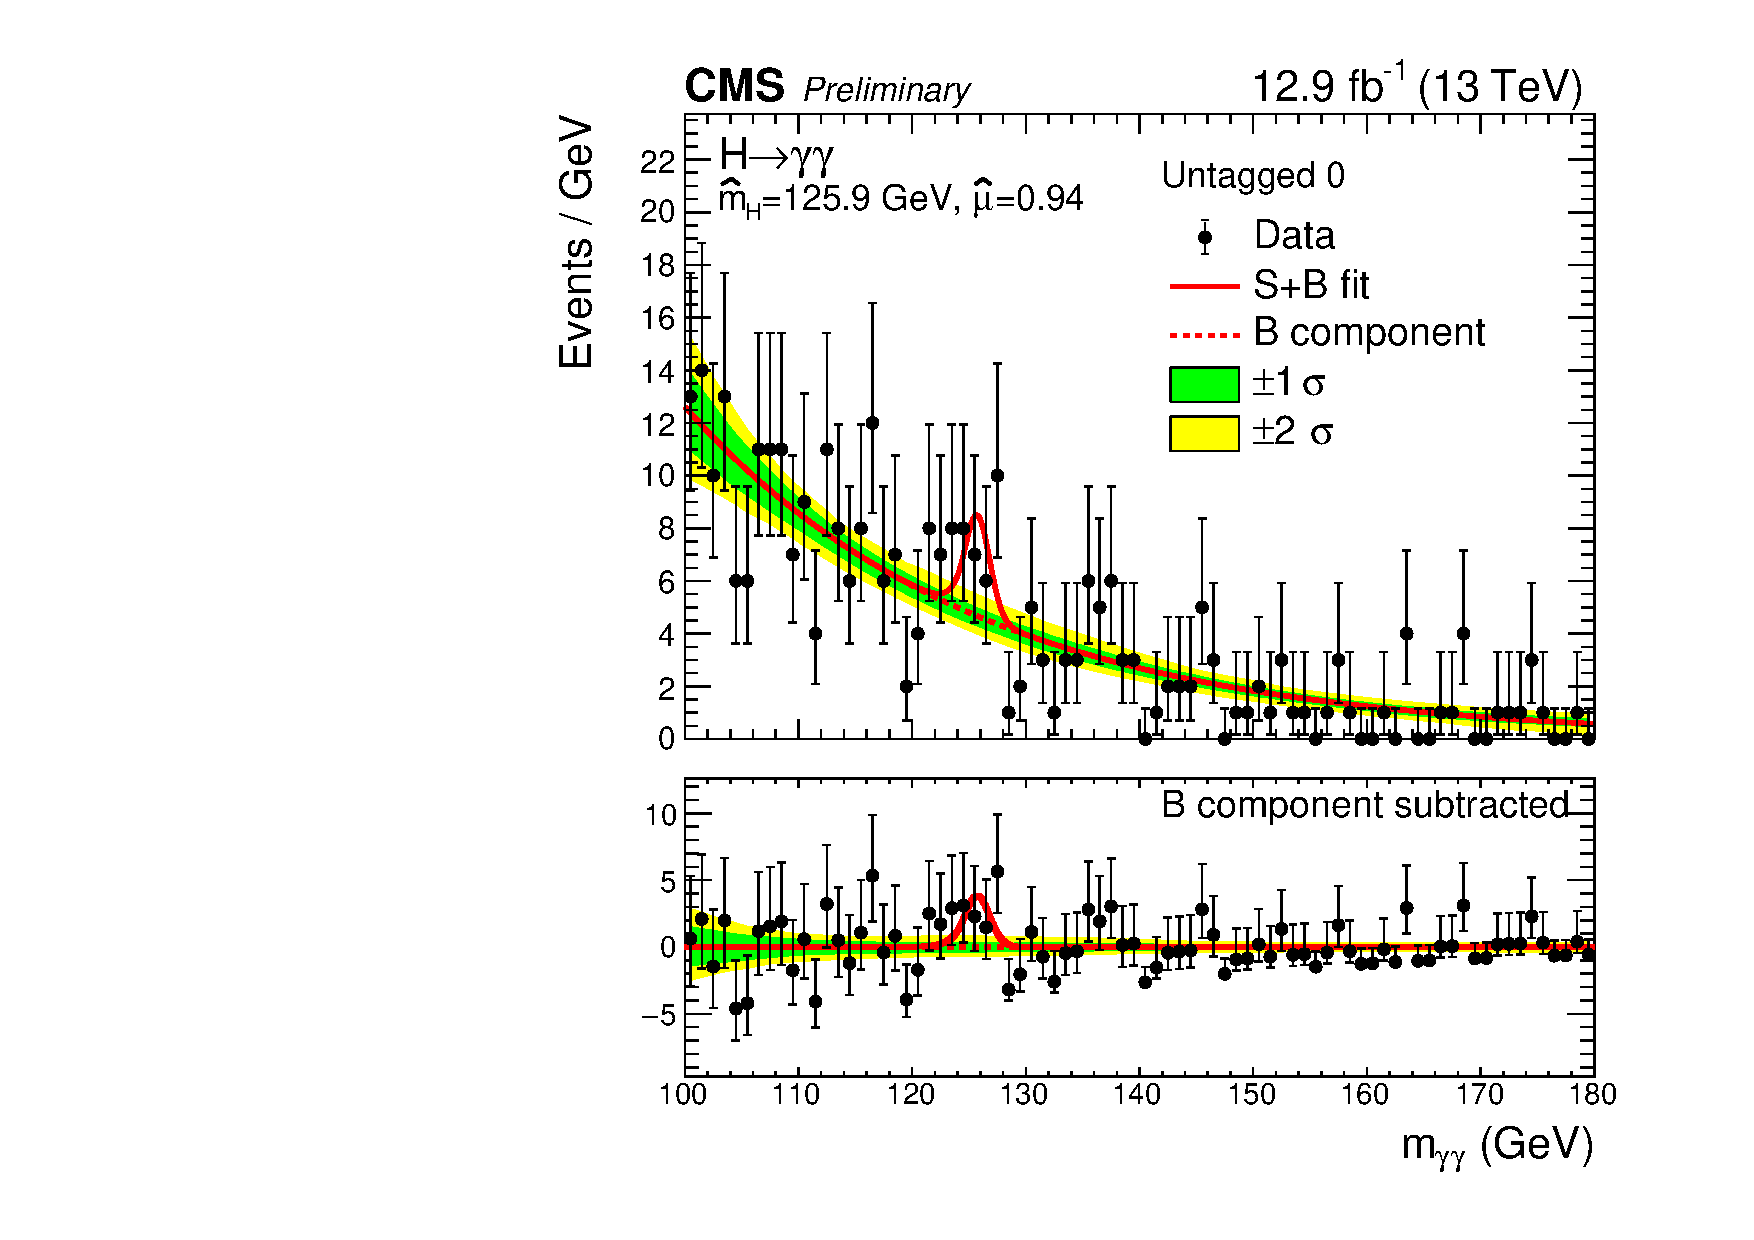
\includegraphics[width=0.49\textwidth]{statandresultsFigures/\whichFig/S_SB_ProfileMH_UntaggedTag_0_13TeV.pdf} 
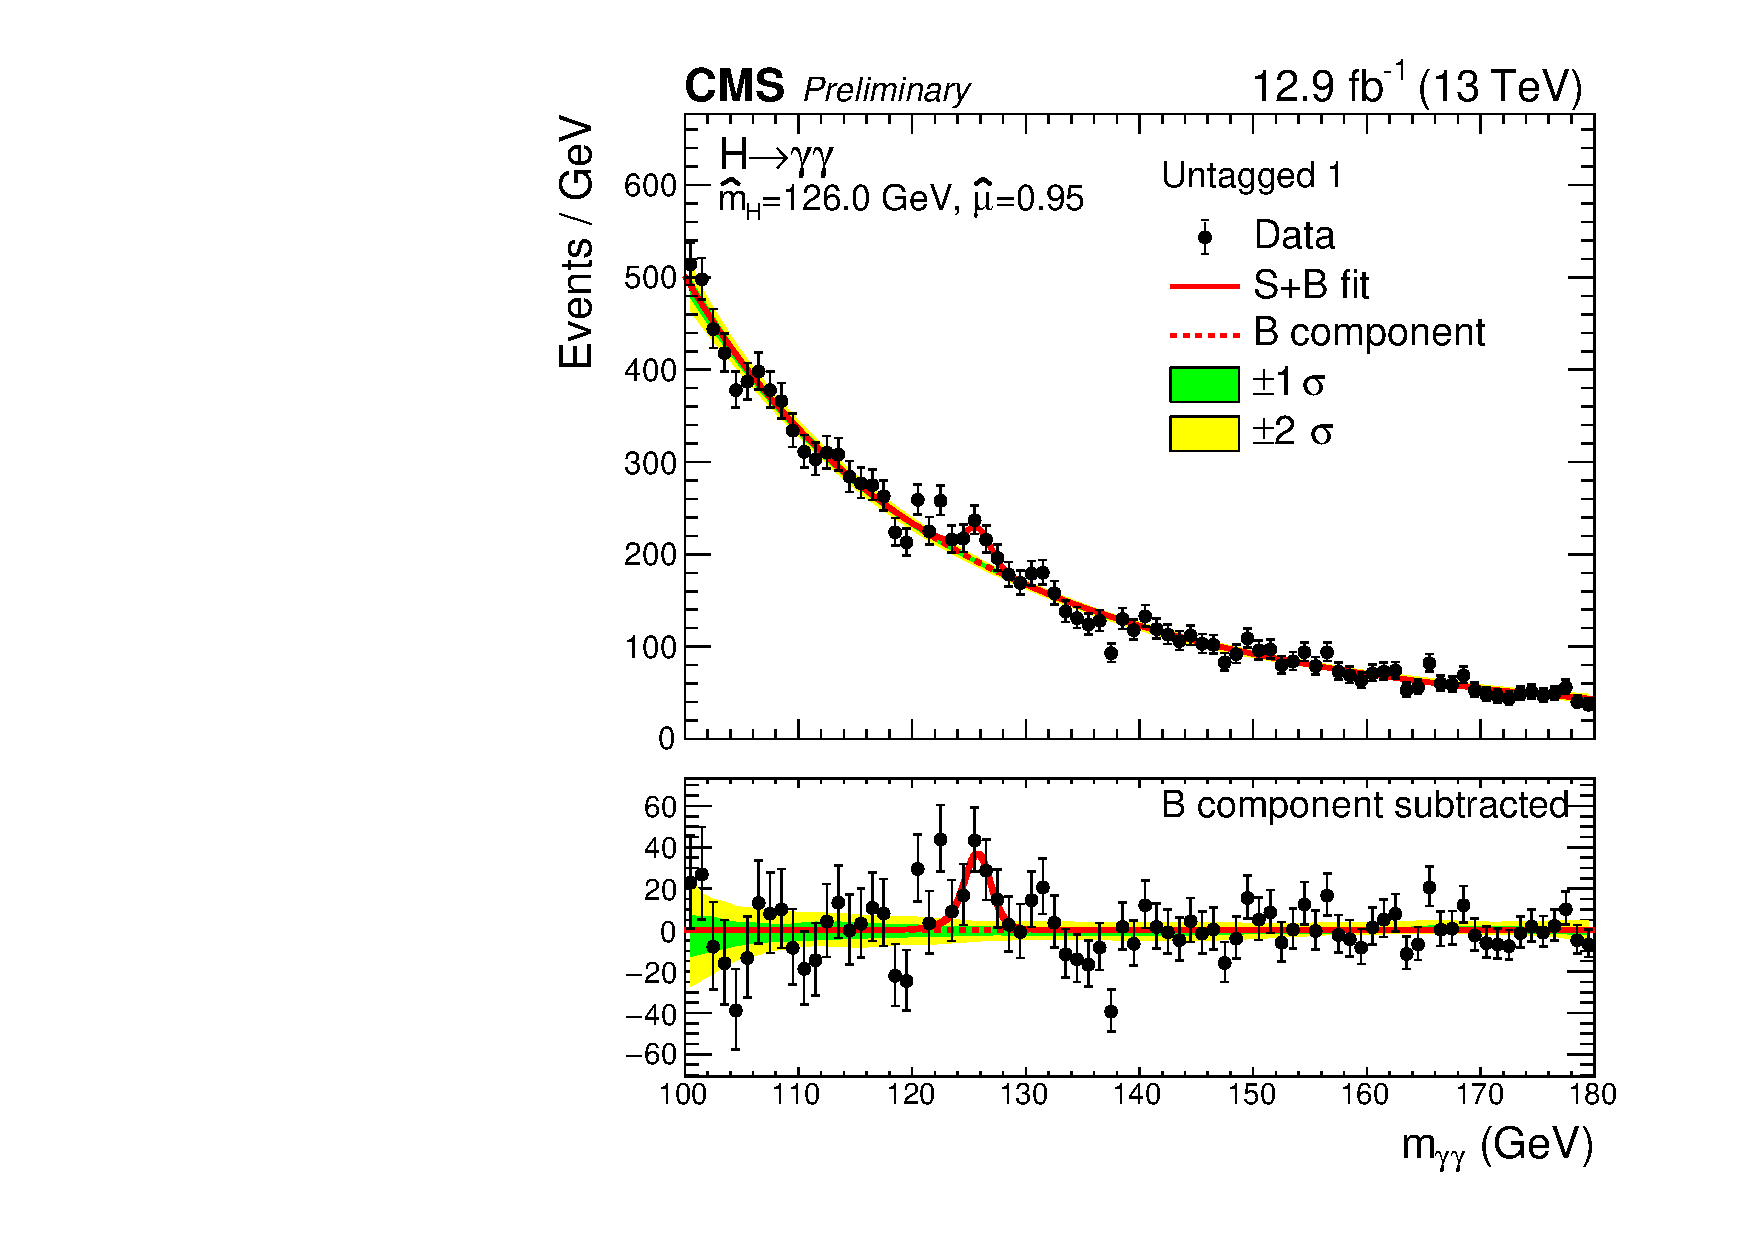
\includegraphics[width=0.49\textwidth]{statandresultsFigures/\whichFig/S_SB_ProfileMH_UntaggedTag_1_13TeV.pdf}\\ 
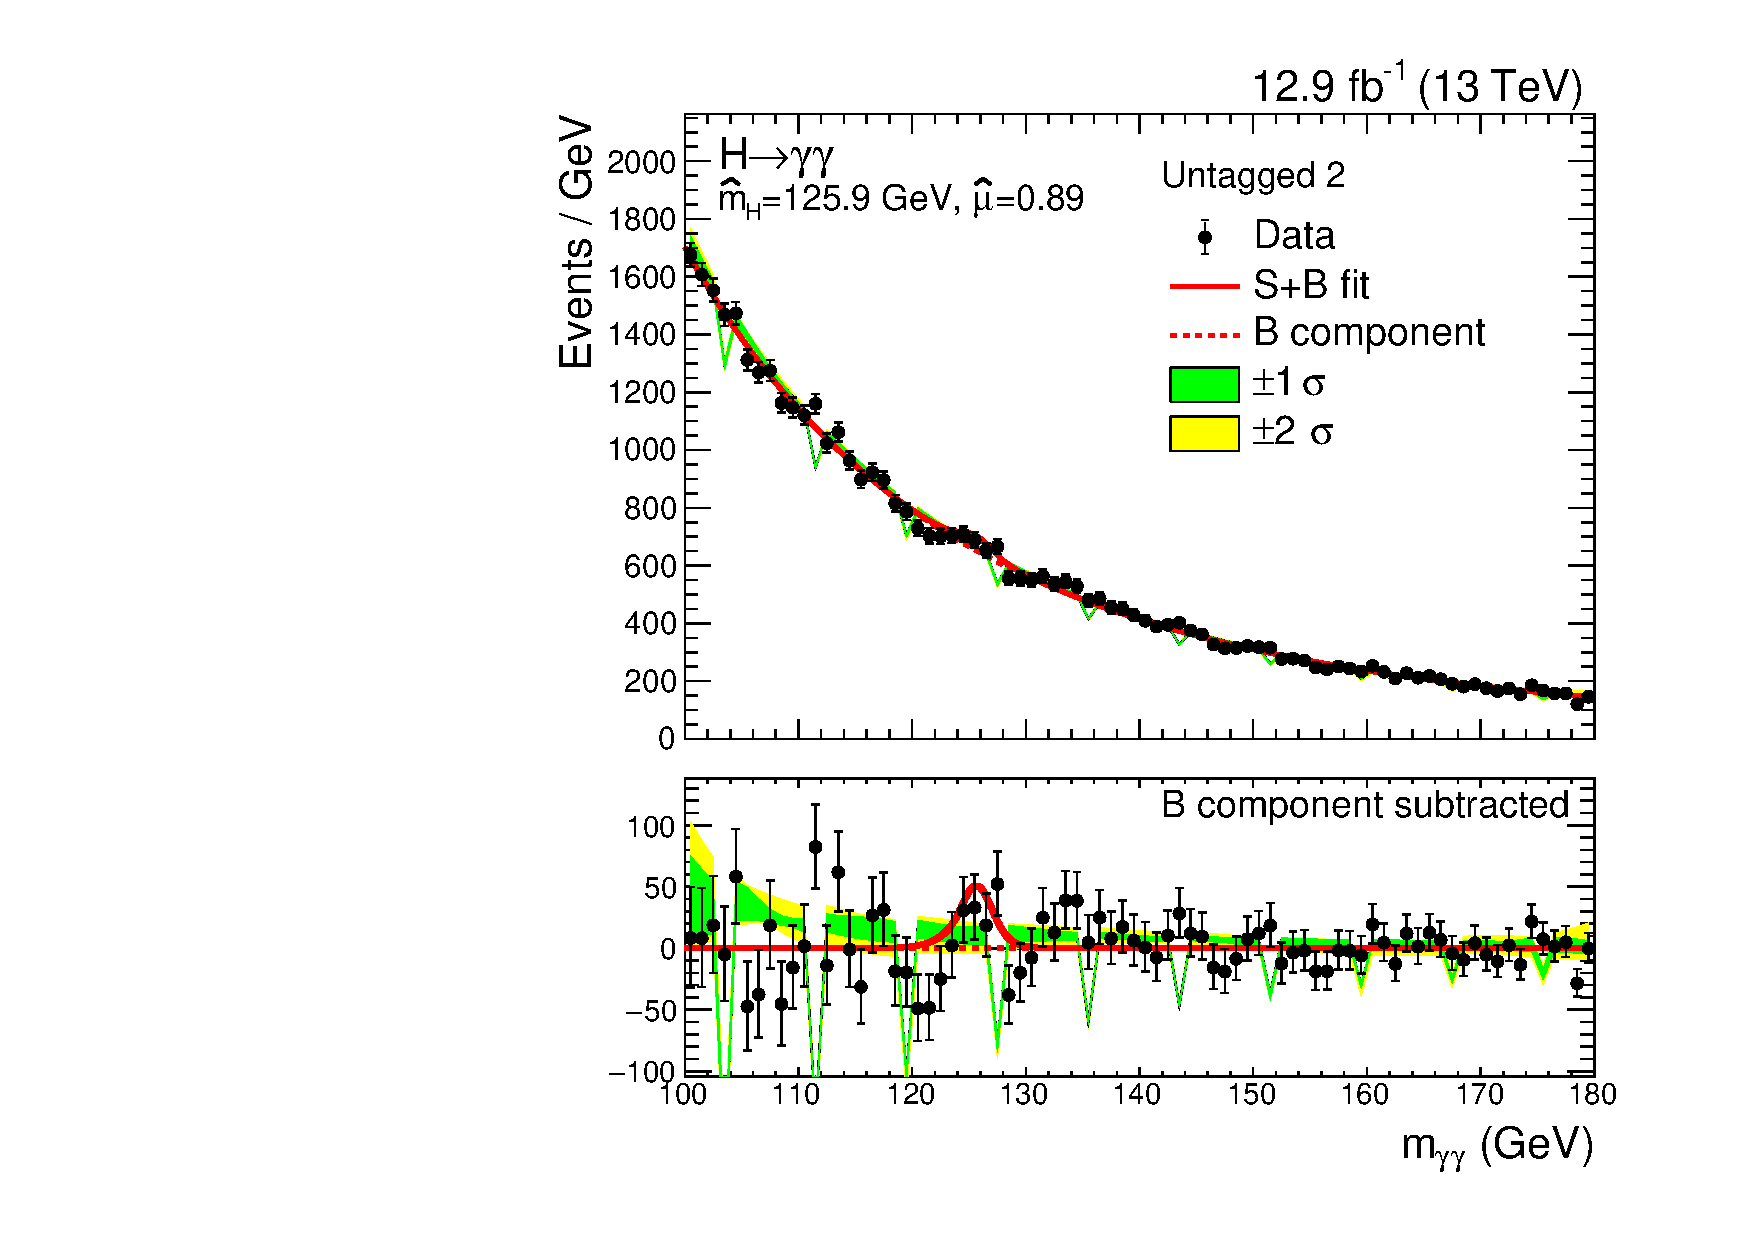
\includegraphics[width=0.49\textwidth]{statandresultsFigures/\whichFig/S_SB_ProfileMH_UntaggedTag_2_13TeV.pdf} 
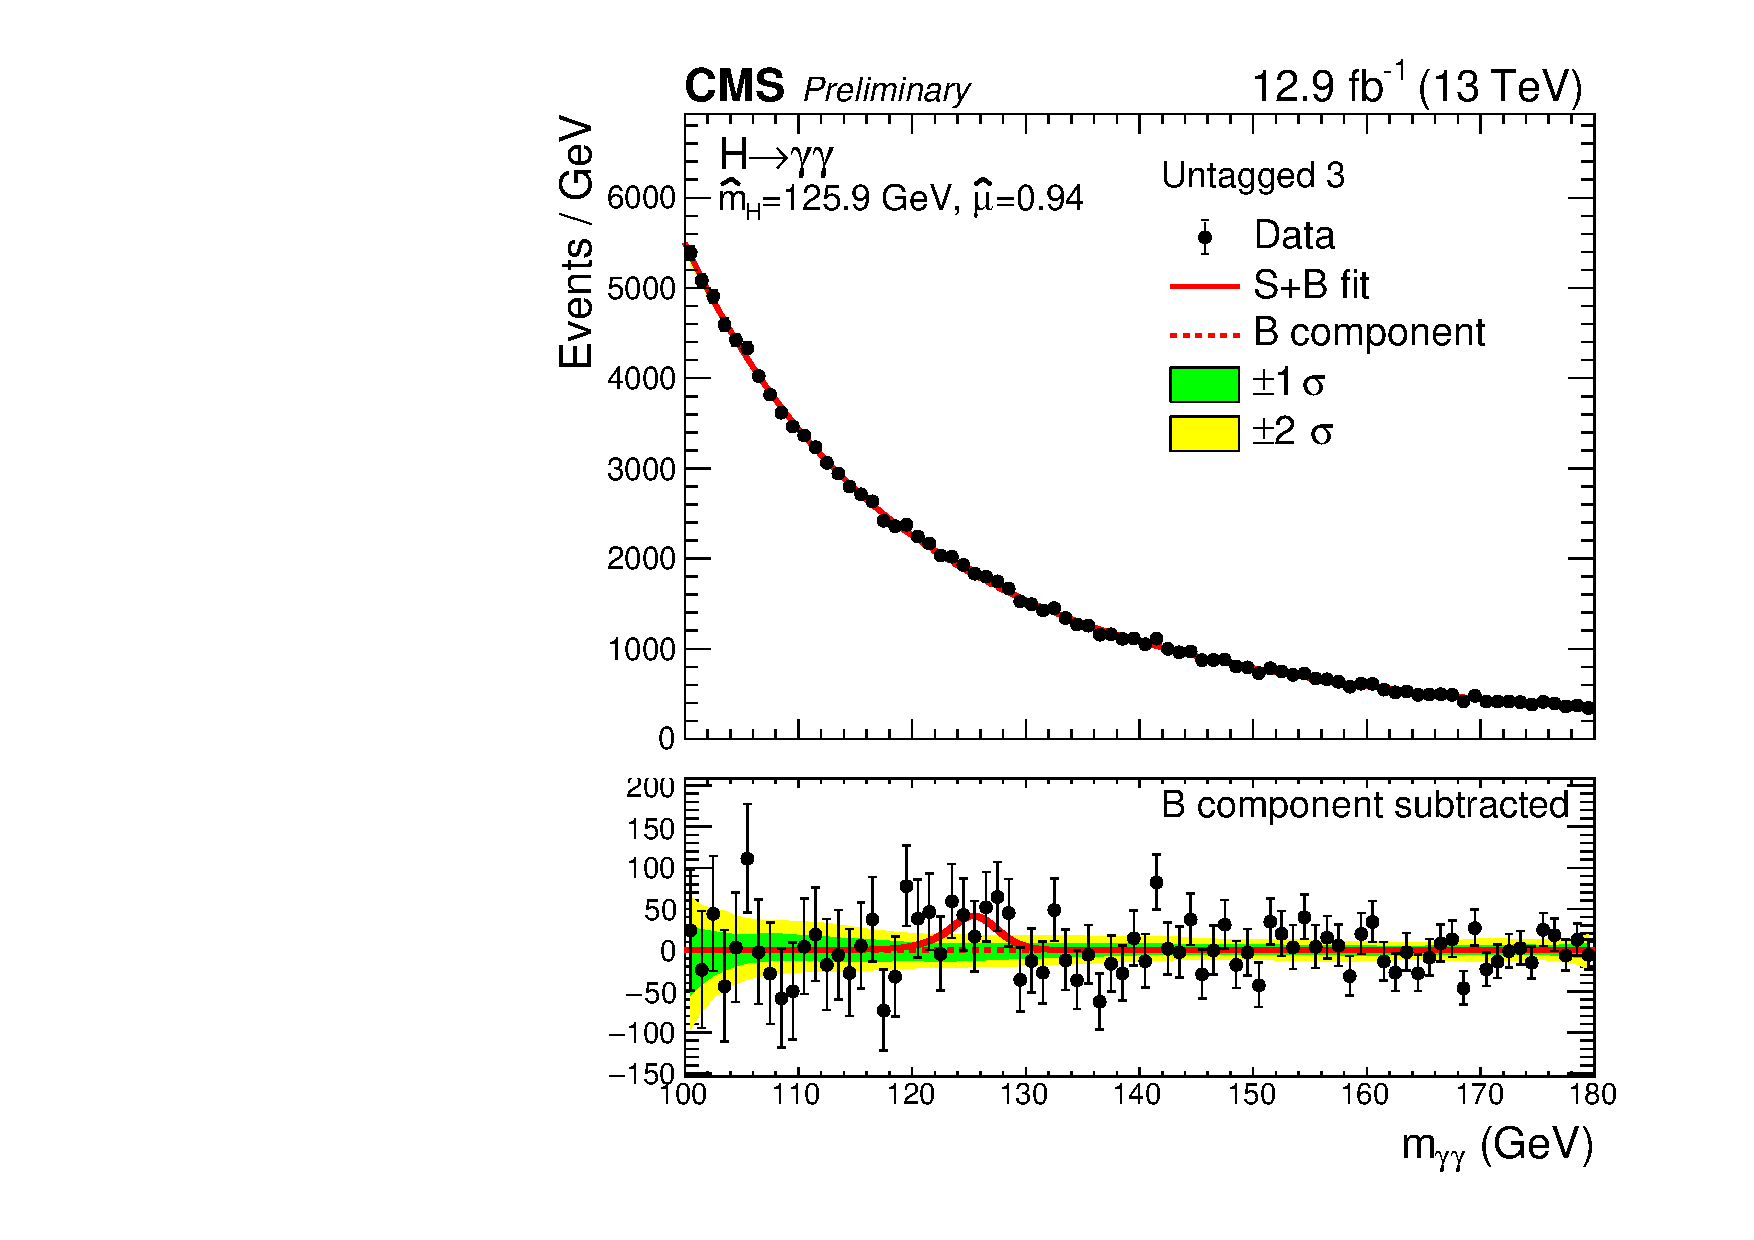
\includegraphics[width=0.49\textwidth]{statandresultsFigures/\whichFig/S_SB_ProfileMH_UntaggedTag_3_13TeV.pdf} \\
\caption{The signal-plus-background fit (solid red line) of the observed \mgg distribution in data (black points) for the \Untagged analysis categories. The background-only fit is shown as a dashed red line, while the green and yellow bands denote the $1\sigma$ and $2\sigma$ uncertainties on the background shape respectively.}

\label{fig:statandresults:s_b_fits}
\end{figure}

\begin{figure}[p]
\centering
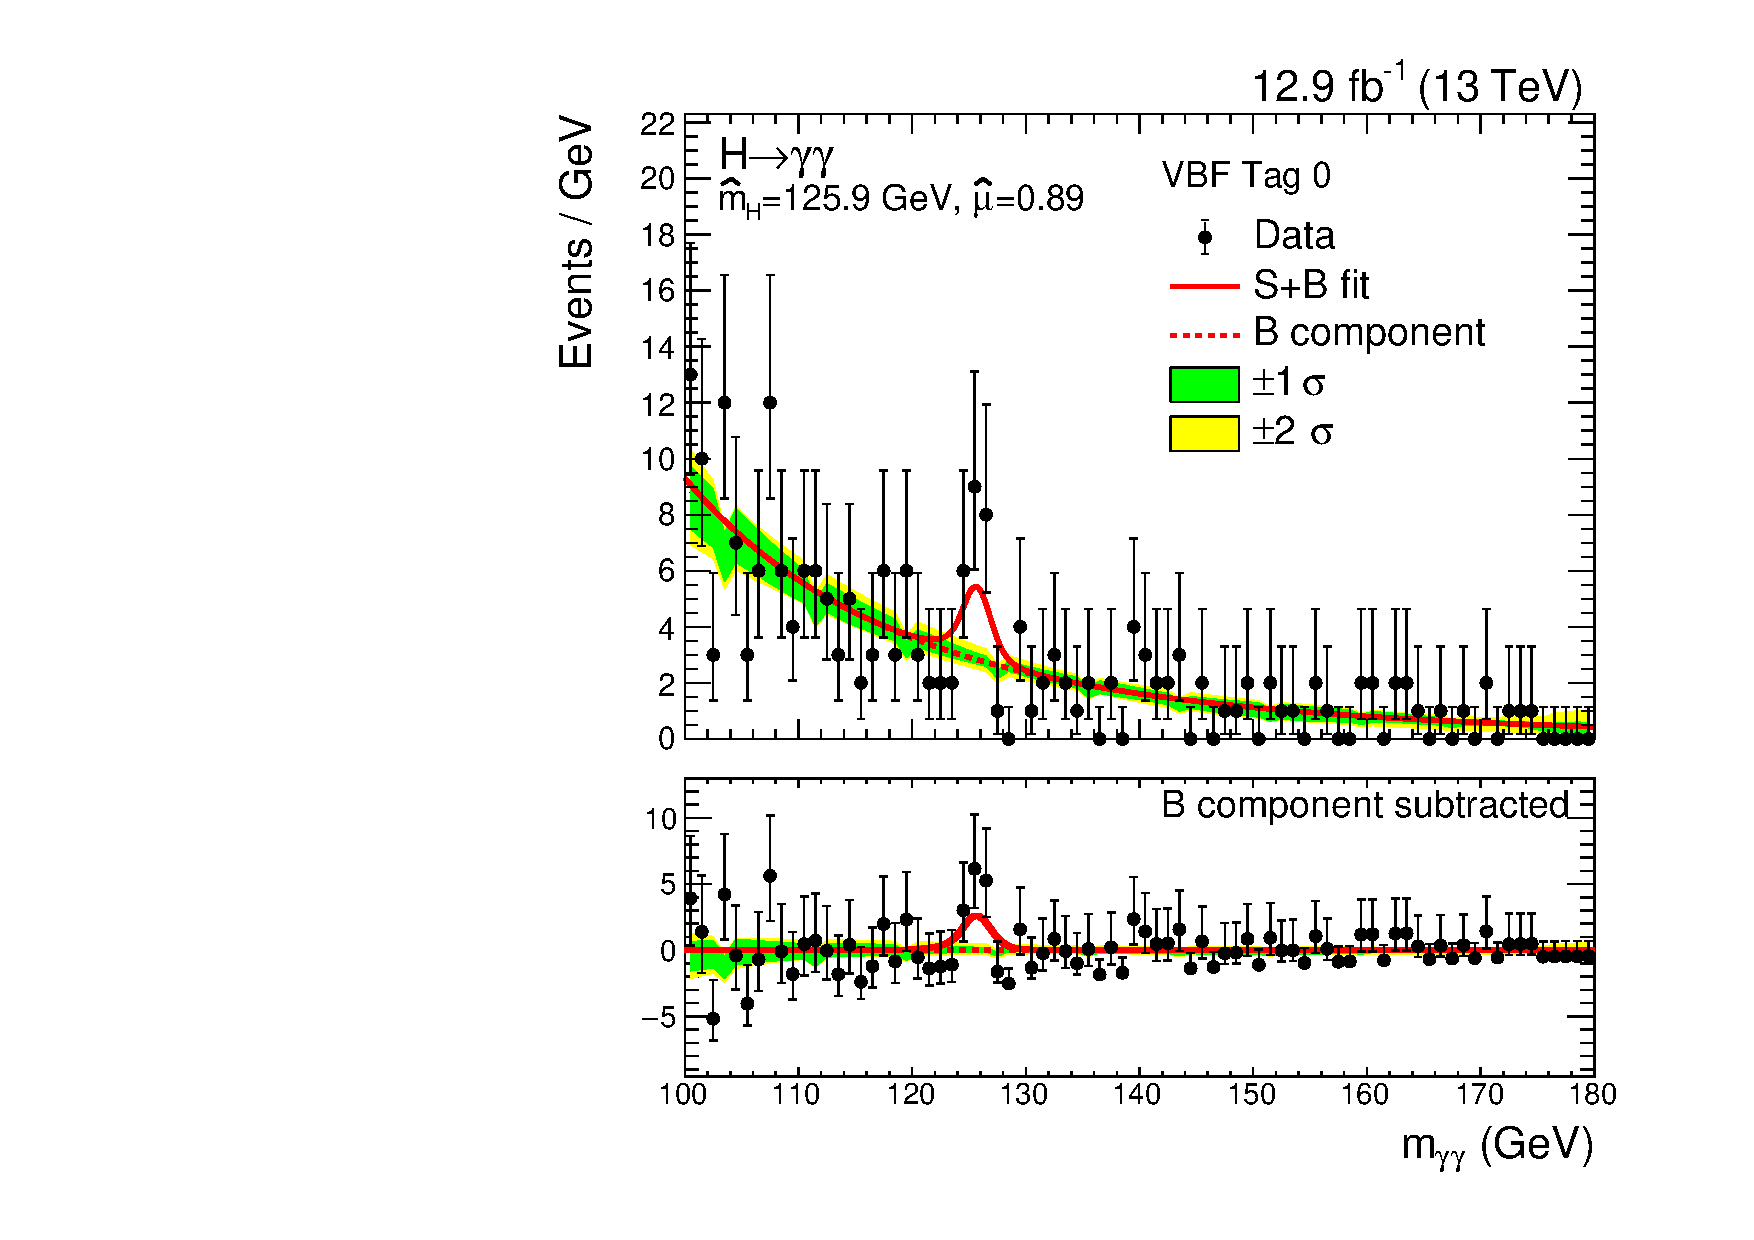
\includegraphics[width=0.49\textwidth]{statandresultsFigures/\whichFig/S_SB_ProfileMH_VBFTag_0_13TeV.pdf} 
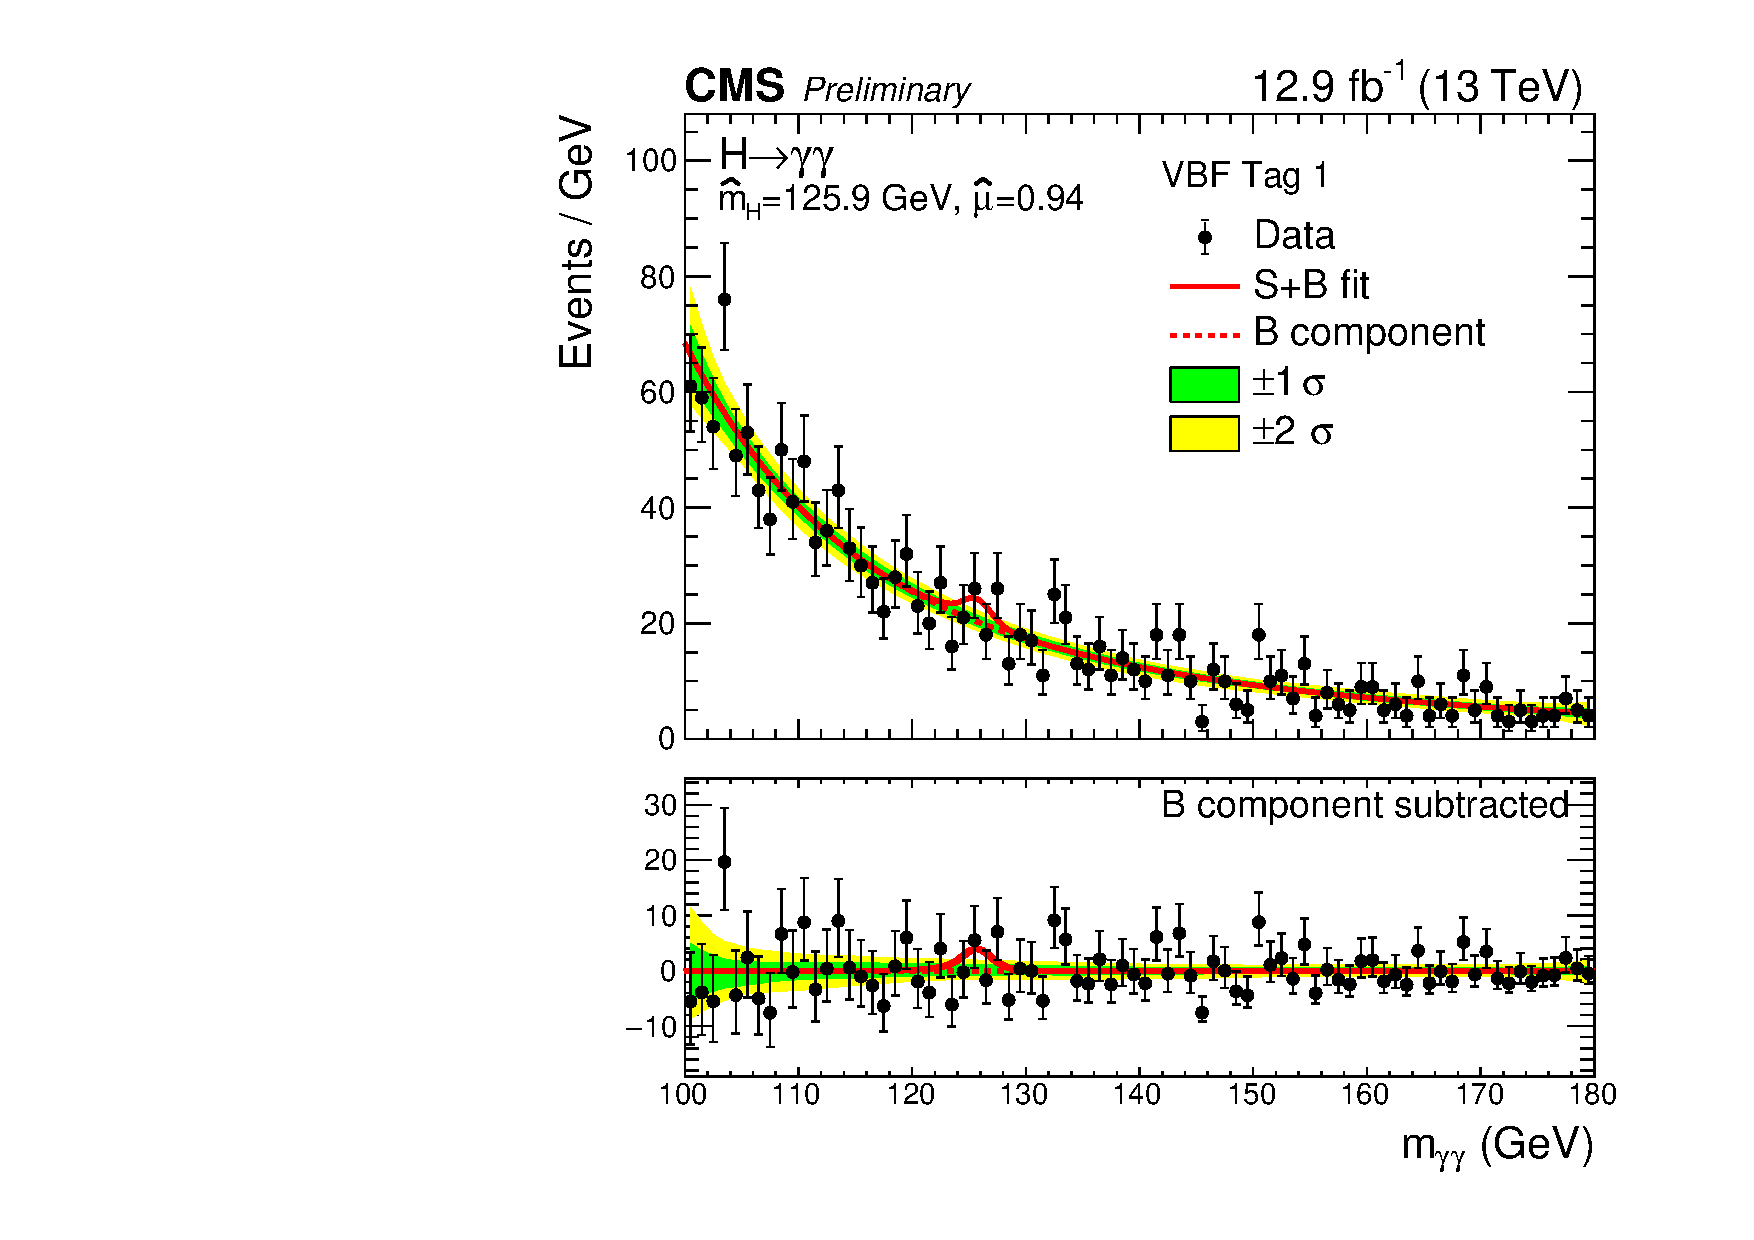
\includegraphics[width=0.49\textwidth]{statandresultsFigures/\whichFig/S_SB_ProfileMH_VBFTag_1_13TeV.pdf} 
%\includegraphics[width=0.3\textwidth]{statandresultsFigures/\whichFig/S_SB_ProfileMH_VBFTag_2_13TeV.pdf} 
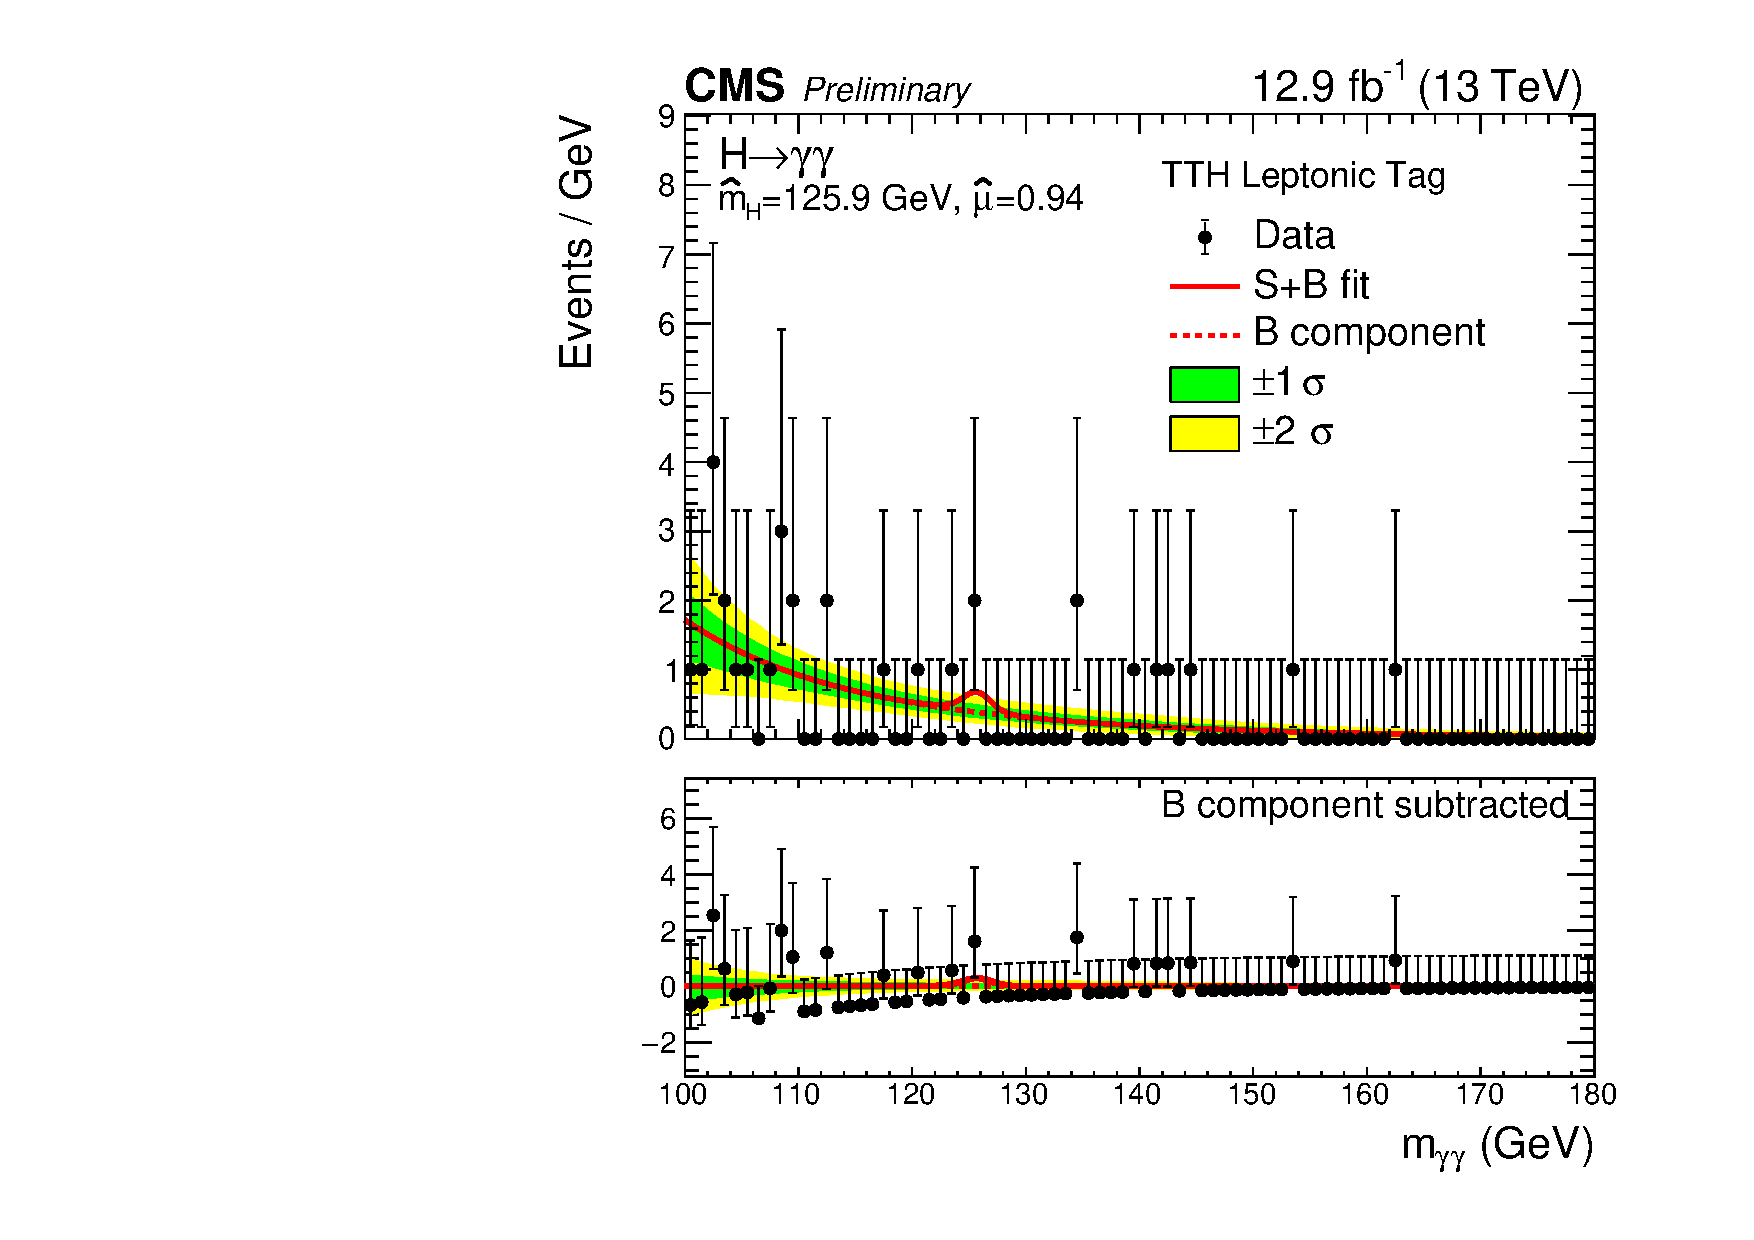
\includegraphics[width=0.49\textwidth]{statandresultsFigures/\whichFig/S_SB_ProfileMH_TTHLeptonicTag_13TeV.pdf} 
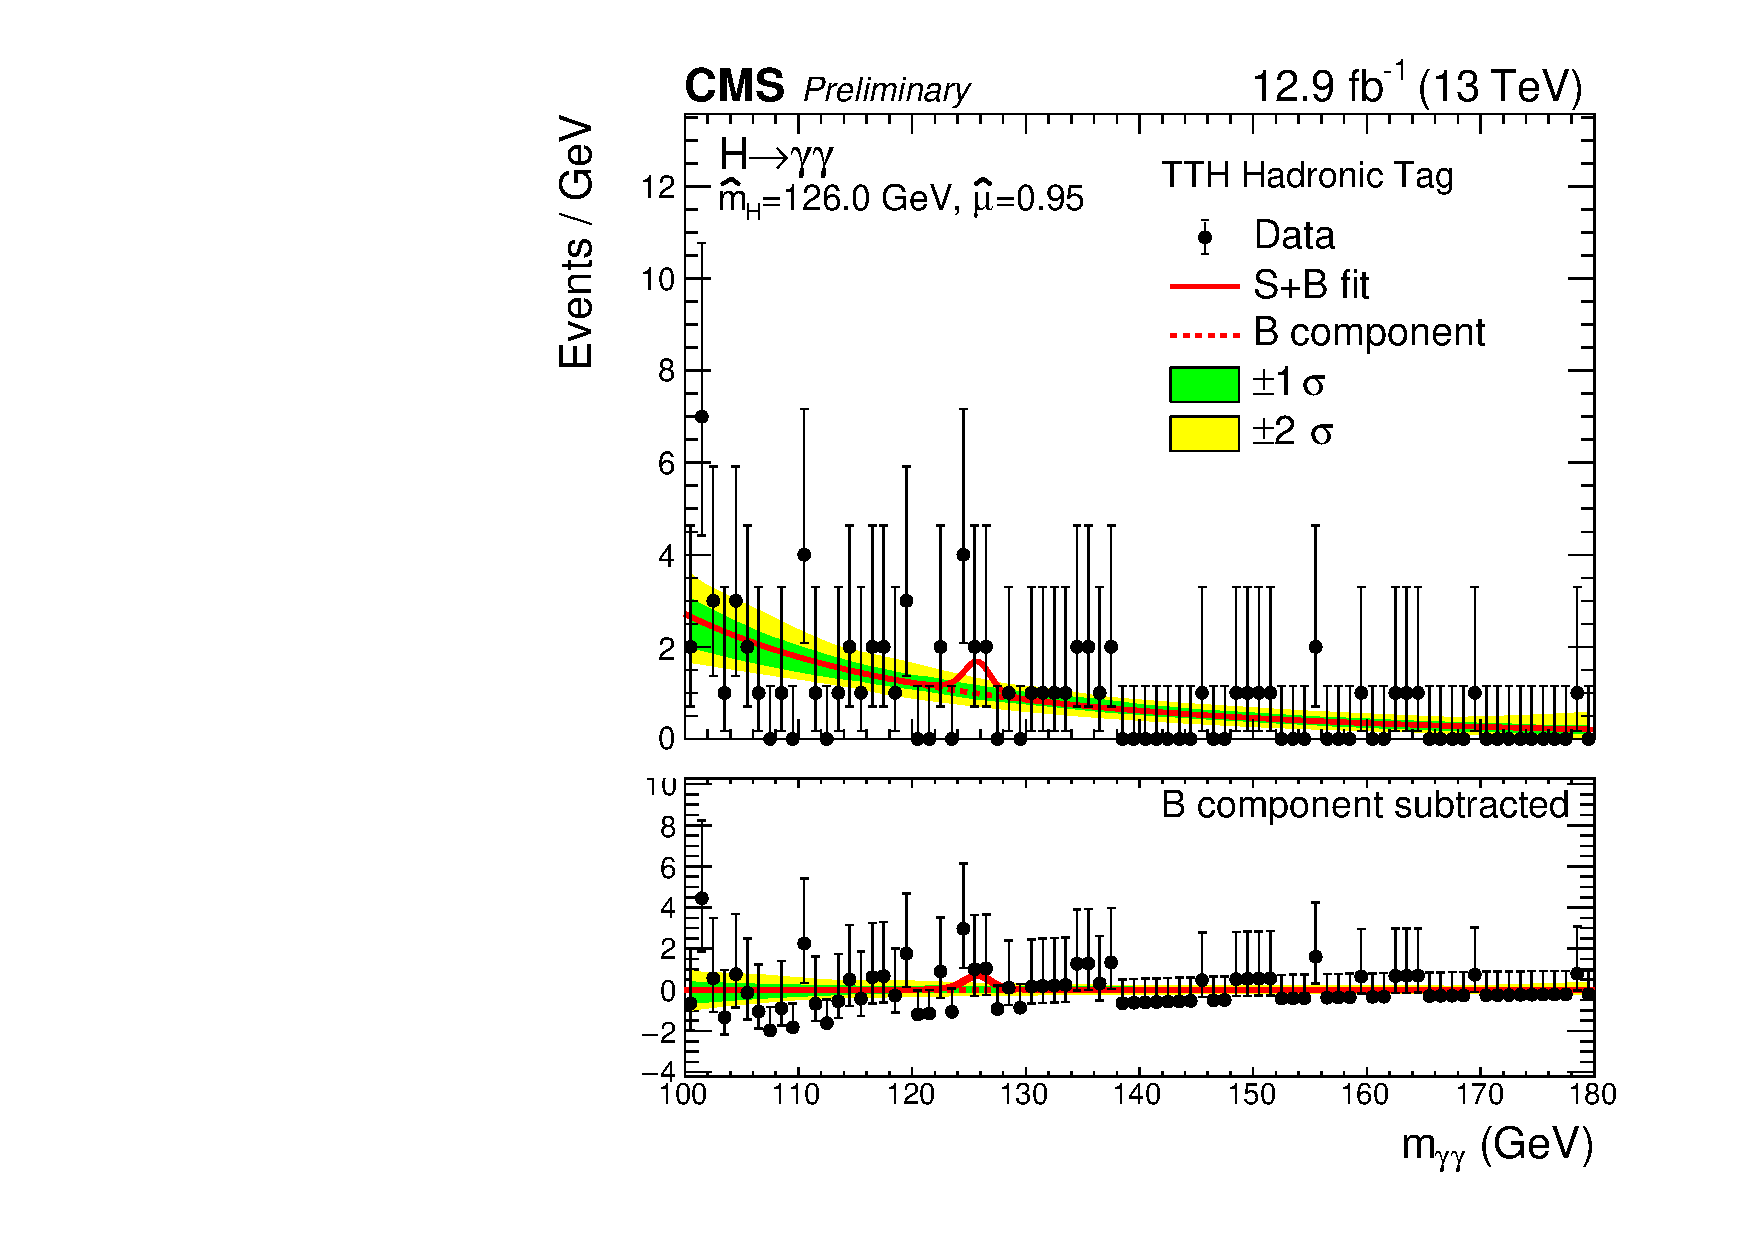
\includegraphics[width=0.49\textwidth]{statandresultsFigures/\whichFig/S_SB_ProfileMH_TTHHadronicTag_13TeV.pdf} \\
%\includegraphics[width=0.3\textwidth]{statandresultsFigures/\whichFig/S_SB_ProfileMH_VHLeptoniclooseTag_13TeV.pdf} 
%\includegraphics[width=0.3\textwidth]{statandresultsFigures/\whichFig/S_SB_ProfileMH_VHMetTag_13TeV.pdf} 
%\includegraphics[width=0.3\textwidth]{statandresultsFigures/\whichFig/S_SB_ProfileMH_VHHadronicTag_13TeV.pdf} \\
%\includegraphics[width=0.3\textwidth]{statandresultsFigures/\whichFig/S_SB_ProfileMH_WHLeptonicTag_13TeV.pdf} 
%\includegraphics[width=0.3\textwidth]{statandresultsFigures/\whichFig/S_SB_ProfileMH_ZHLeptonicTag_13TeV.pdf} 
\caption{The signal-plus-background fit (solid red line) of the observed \mgg distribution in data (black points) for the \VBFTag and \TTHTag analysis categories. The background-only fit is shown as a dashed red line, while the green and yellow bands denote the $1\sigma$ and $2\sigma$ uncertainties on the background shape respectively.}

\label{fig:statandresults:s_b_fits_bis}
\end{figure}

\begin{figure}[hpt!]
\centering
\subfloat[Direct sum]{
 \label{fig:statandresults:s_b_fits_direct_sum}
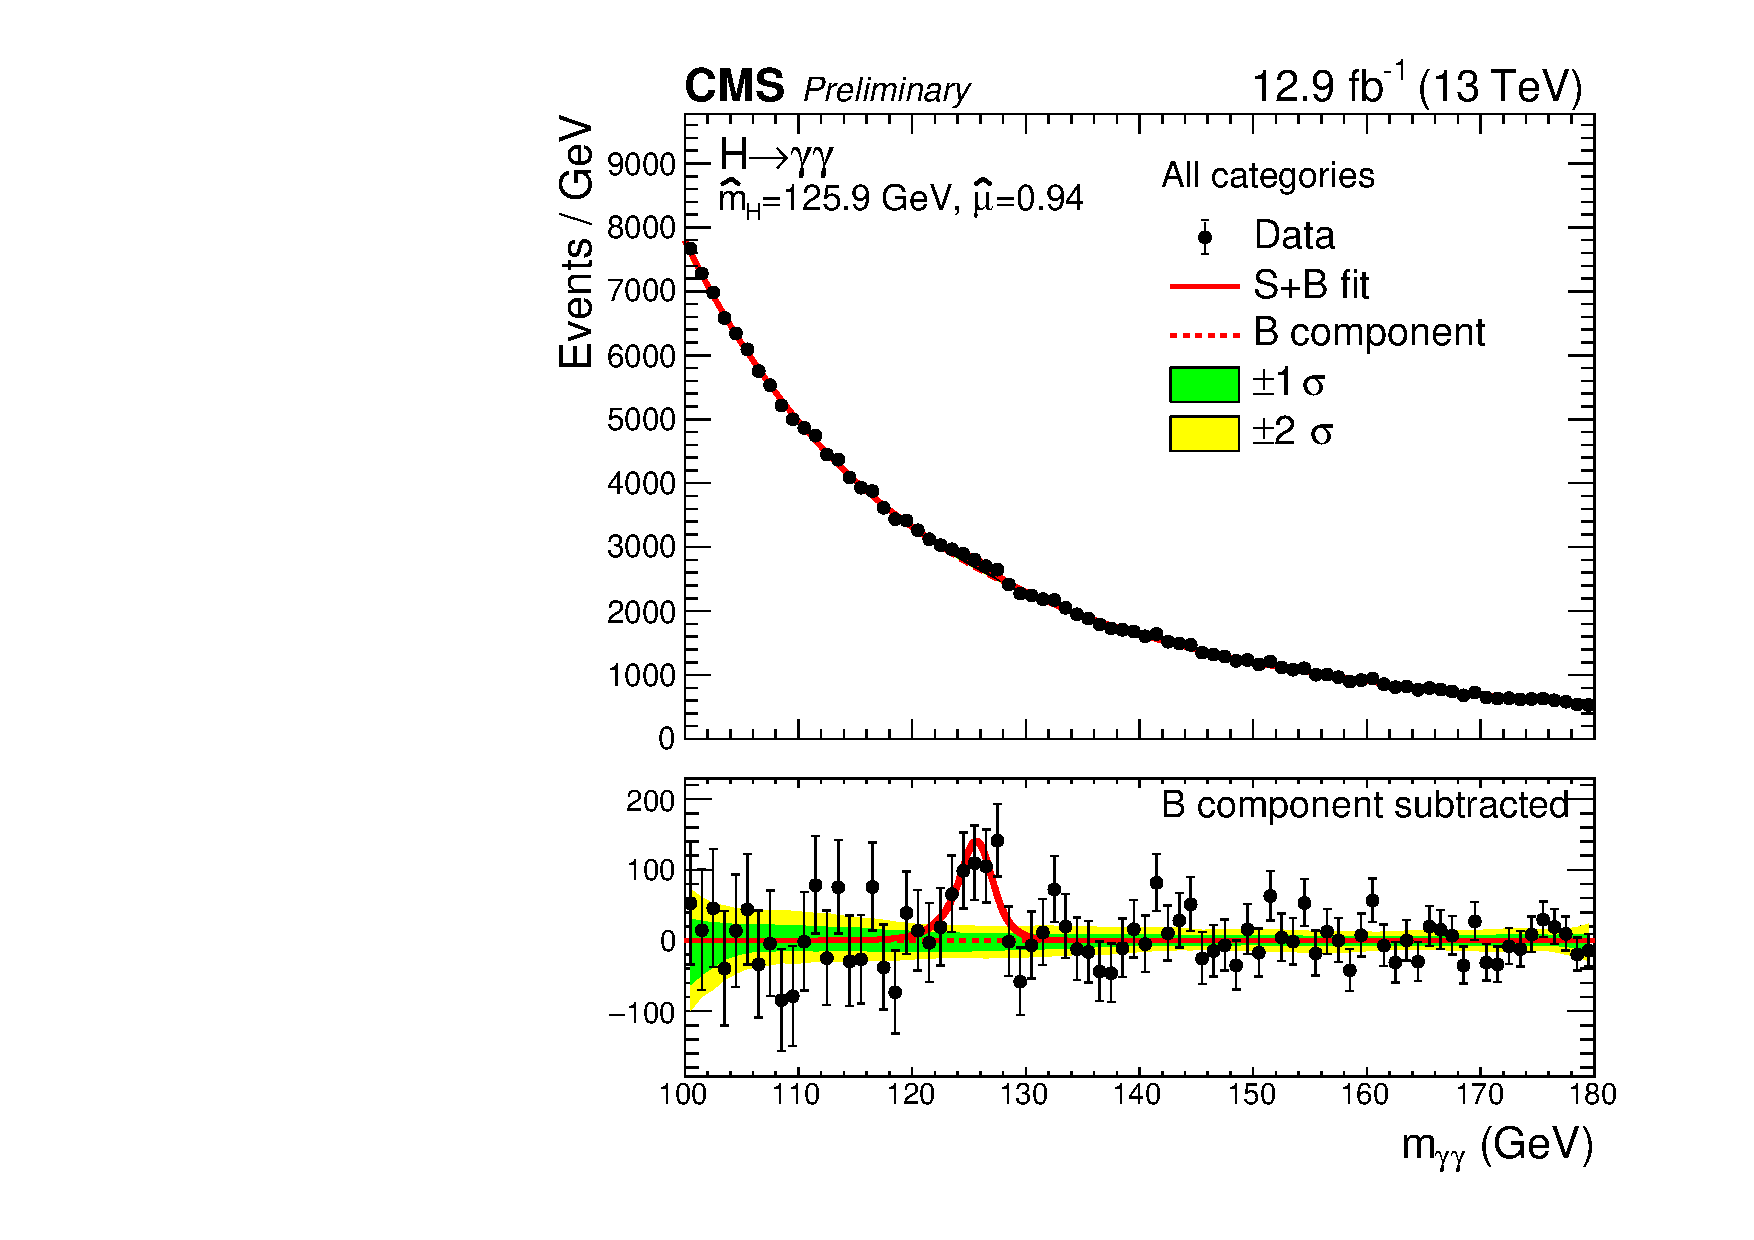
\includegraphics[width=0.59\textwidth]{statandresultsFigures/\whichFig/S_SB_ProfileMH_combcat_unweighted.pdf}}\\
\subfloat[S/(S+B) weighted sum]{
 \label{fig:statandresults:s_b_fits_s_sb_sum}
\includegraphics[width=0.59\textwidth]{statandresultsFigures/\whichFig/S_SB_ProfileMH_combcat_weighted.pdf}}
\caption{The signal-plus-background fit (solid red line) of the observed \mgg distribution in data (black points) for all categories combined, either using a direct sum (a) or a sum weighted by the $S/(S+B)$ in $\pm 1 \effSigma$ around the best-fit value of \mH (b). The background-only fit is shown as a dashed red line, while the green and yellow bands denote the $1\sigma$ and $2\sigma$ uncertainties on the background shape respectively.}

\label{fig:statandresults:s_b_fits_sum}
\end{figure}

The best-fit values of the \POI\s are found to be $\hat{\mu}=\bestFitGlobalMu$ and $\hat{\mH}= \bestFitGlobalMH\GeV$ (the best-fit values in~\cite{CMS-PAS-HIG-16-020} were $0.95$ and $126.0$ respectively). The best-fit parametrisation qualitatively indicates the presence of an excess of data in the same place in the \mgg distributions in all analysis categories. When the categories are summed, particularly when weighted by their $S/(S+B)$, the presence of a narrow resonance above the falling background spectrum is visible by eye. The best-fit of the signal-plus-background model to the observed data therefore suggests a \SM-like Higgs boson signal in the data, although a full statistical assessment needs to be undertaken to quantify the size of the excess, taking into account the sources of systematic uncertainty which enter the analysis. 


\section{Significance of observation}
\label{sec:statandresults:significance}

Given the best-fit value of the signal strength $\hat{\mu}= \bestFitGlobalMu$ determined in \Sec~\ref{sec:statandresults:bestfit}, a frequentist approach is used to determine the degree of certainty with which the null hypothesis (that there is no Higgs boson) can be rejected in favour of an alternative hypothesis (that a \SM-like Higgs boson exists). The hypotheses can be formulated in terms of the signal strength: the null hypothesis $H_{0}$ corresponds to the case where $\mu=0$, while the alternative hypothesis $H_{\mu}$ corresponds to $\mu > 0$. 

A statistical test is constructed by specifying a critical region $w$ of the data space, such that for a given set of observed data $\mgg^{obs}$:
\begin{equation}
P(\mgg^{obs} \in w | H_{0} ) \leq \alpha,
\end{equation}
where $P(\mgg^{obs} \in w | H_{0} ) $ is the probability (assuming that $H_{0}$ is correct), of observing the data inside the critical region $w$, and $\alpha$ is a small predetermined threshold~\cite{Cowan}. 

The statistical power $\beta$ of the test is the probability of accepting $H_{0}$ when it is false and the alternative $H_{\mu} $ is true. This is given by:
\begin{equation}
P(\mgg^{obs} \in w | H_{\mu} ) = 1 - \beta.
\end{equation}
The critical region is be chosen such that the power $\beta$ of the test is maximised for a given $\alpha$, to ensure that if $\mgg^{obs} \in w$, then $H_{0}$ has a low probability of being true while $H_{\mu}$ has a high probability of being true. 

A common choice, which is found to maximise $\beta$~\cite{Cowan}, is to define the critical region in terms of a test statistic $q_{\mu}$, corresponding to the difference between the best-fit \NLL and the \NLL (abbreviated as \DNLL) evaluated for a particular $\mu$. The test statistic is defined explicitly as:
\begin{equation}
\label{eq:statandresults:test_statistic}
q_{\mu} = \begin{cases} 
% -2 \ln \mathcal{L}(\mu,\hat{\mH}^{\mu} ; \hat{\mathbf{n}}^{\mu}| \mgg^{obs})- 2\ln\mathcal{L}(\hat{\mu},\hat{\mH} ;\hat{\mathbf{n}}| \mgg^{obs} ) & \text{when } \hat{\mu} \geq 0, \\
 -2 \ln \mathcal{L}(\mu,\mH; \hat{\mathbf{n}}^{\mu}| \mgg^{obs})- 2\ln\mathcal{L}(\hat{\mu},\mH;\hat{\mathbf{n}}| \mgg^{obs} ) & \text{when } \hat{\mu} \geq 0, \\
 0 & \text{when } \hat{\mu} < 0, 
 \end{cases}
\end{equation}

%where $\hat{\mH}^{\mu}$ and 
where $\hat{\mathbf{n}}^{\mu}$ denotes the best fit $\mathbf{n}$ for a fixed value of $\mu$. 
%In this case, \mH is allowed to float with a flat constraint, and is said to be \emph{profiled}. The test statistic can be modified to evaluate the \DNLL for a given \mH hypothesis by fixing it to a particular value instead. 
When trying to exclude hypothesis $H_{0}$, the test statistic $q_{0}$ in particular is used to define a critical region. In the limit of a large sample of data, the probability distribution function of the test statistic ($f_q$), is Gaussian. The fact that $q_{0} =0$ for $\hat{\mu} < 0$ reflects the fact that only excesses in the data are regarded as significant. This simplifies the definition of the critical region, since increasingly large values of $q_{0}$ indicate increasing incompatibility with $H_{0}$, and therefore only the right-hand tail of $f_q$ is considered when assessing probabilities. Assuming $H_{0}$, the probability of obtaining a value of $q^{{obs}}_{0}$ (corresponding to observed data $ \mgg^{obs}$) or higher is given by the integral of $f_q$ from $q^{{obs}}_{0}$ to infinity. This probability is commonly referred to as the \pvalue. We can therefore define the critical region as: 
\begin{equation}
w = \{ \mgg^{obs} : \int_{q^{{obs}}_{0}}^{+\infty} f_q(q_{0}) dq_0 \leq \alpha \},
\end{equation}

In particle physics experiments, the threshold $\alpha$ to reject the null hypothesis is typically $2.87 \times 10^{-7}$. If expressed as the number of standard deviations that a Gaussian-distributed variable would fluctuate to give the same \pvalue, then this threshold is $5\sigma$.

The test statistic $q_{\mu}$ in \Eq~\ref{eq:statandresults:test_statistic} is implicitly defined for a particular assumption on the value of \mH. This ensures that only excesses compatible with the Higgs boson signal distribution for that particular value of \mH are regarded as significant. In other words, only localised excesses in the \mgg spectrum will lead to a small \pvalue. Thus, in this context we refer to local \pvalue\s, which represent the probability that a statistical fluctuation in the observed background distribution gave rise to a localised excess consistent with the signal model at the assumed \mH. The definition of $H_{\mu}$ thus also depends on the assumed value of \mH. In particular, $H_{\mu}$ is the hypothesis that there exists a Higgs boson with mass \mH and signal strength $\mu$. If the observed data fall in the critical region for a given value of \mH, then the null hypothesis (that there is no Higgs boson, regardless of its mass) is rejected in favour of $H_{\mu}$ for that particular \mH. This is not, however, the same as saying that the Higgs boson has that particular value of \mH. The correct statement is that the alternative hypothesis, assuming \mH, is more likely than $H_{0}$ given the data, and that $H_{\mu}$ assuming a different \mH could be yet more likely.

The local \pvalue is therefore evaluated separately, given the observed data, for different assumptions about the value of \mH in the range 120-130\GeV in 0.1\GeV steps. The result is shown in \Fig~\ref{fig:statandresults:pval}. The black solid line represents the local \pvalue scan for the observed data. The dashed lines represent the expected local \pvalue\s for a \SM Higgs boson. These are obtained by generating an Asimov dataset~\cite{Cowan:2010js} from the best-fit background-only model and a signal of strength $\mu=1$, and then performing a signal-plus-background fit and following the same procedure as for observed data. For the blue dashed line, the signal was injected at $\mH=125.09\GeV$ (the best fit value from the previous combined \RunI measurement by \CMS and \ATLAS~\cite{PhysRevLett.114.191803}), while for the red dashed line the signal was injected at the corresponding \mH for each step. 


\begin{figure}[ht!]
\centering
\includegraphics[width=0.9\textwidth]{statandresultsFigures/\whichFig/pval13TeV-observed.pdf} 
\caption{The local \pvalue for the observation as a function of the Higgs boson mass (black), shown with the expected local \pvalue\s for a SM Higgs boson, across the range 120-130\GeV. The expected local \pvalue\s are obtained using Asimov datasets. The blue dashed line shows the expected local \pvalue when the mass of the injected signal is $\mH=125.09\GeV$, while the red line shows the maximum significance for any injected signal in the range of $120$ to $130\GeV$.}

\label{fig:statandresults:pval}
\end{figure}

The local observed significance at the \RunI best fit ($\mH=125.09\GeV$) is $\obsSigAtRunIBF\sigma$, where $\expSigAtRunIBF\sigma$ was expected for the \SM Higgs boson. The maximum local observed significance is found at $\bestFitGlobalMH\GeV$, corresponding to $\obsSigAtMin\sigma$ where $\expSigAtMin\sigma$ was expected (these results are consistent with~\cite{CMS-PAS-HIG-16-020} to within one unit of the smallest quoted decimal place). % $5.6\sigma$ at $\mH=125.09\GeV$ is where $6.2\sigma$ was expected, and maximum local observed significance at $\mH=126.0\GeV$, corresponding to $6.1\sigma$.
Since the observed data fall in the critical region where at least one \mH assumption yields a local significance above $5\sigma$ (i.e \pvalue is less than $2.87 \times 10^{-7}$), the null hypothesis that there is no Higgs boson is rejected in favour of the alternative hypothesis that there exists a Higgs boson. Therefore, the data correspond to an observation of the Higgs boson decaying to photons.

The maximum significance of the observation in this analysis occurs near $\mH=126.0\GeV$, which is somewhat different from the combined best-fit \mH measured in \RunI. %world average values of $125.09\pm0.24\GeV$ from the combination of \CMS and \ATLAS results from \RunI ~\cite{PhysRevLett.114.191803}. 
However, the results which are presented here do not comprise a measurement of the Higgs boson mass, as the data were not reprocessed with the final set of \ECAL calibrations and tuning of the \PhoEnergyBdt which are required for a precision measurement. %As can be seen from \Table~\ref{tab:model:systematics}, the corresponding shape nuisances have a negligible effect on the measurements of the signal strength and related quantities, and therefore these considerations do not invalidate the results presented in this thesis.

\section{Measurements of the signal strength}
\label{sec:statandresults:sigstrength}
\subsection{Global signal strength}
\label{sec:statandresults:sigstrength_global}

One of the advantages of using \DNLL as a test statistic is that to a very good approximation, the $\pm 1 \sigma$ and $\pm 2 \sigma$ uncertainty on the measured value of a \POI can be obtained by finding the values of the \POI for which $\DNLL=1$ and $\DNLL=4$ respectively~\cite{Cowan}. %$q_{\mu}=q_{\hat{\mu}}+1$~\cite{Cowan}.
This fact is used to produce a measurement of the global signal strength $\mu$. 

Two modifications are made to the definition of the test statistic in \Eq~\ref{eq:statandresults:test_statistic}. First, the \mH parameter is profiled in the minimisation at each step, which means that it is allowed to float with a flat constraint. Second, the requirement that the test-statistic is nonzero only for positive values of $\hat{\mu}$ is relaxed, since this was a enforced to simplify the calculation of \pvalue\s. The new definition of the test statistic is therefore given by: 
\begin{equation}
\label{eq:statandresults:test_statistic_profMH}
q_{\mu} = -2 \ln \mathcal{L}(\mu,\hat{\mH}^{\mu} ; \hat{\mathbf{n}}^{\mu}| \mgg^{obs})- 2\ln\mathcal{L}(\hat{\mu},\hat{\mH} ;\hat{\mathbf{n}}| \mgg^{obs} ), 
\end{equation}
where $\hat{\mathbf{\mH}}^{\mu}$ denotes the best-fit \mH for a fixed value of $\mu$. %Other treatements of the \mH paramater are possible (for instance, fixing it to the central value from the current best measurement, or Gaussian-constraining it within the uncertainties of the best measurement), but these do not signifiancelty change the final measurement of the signal strength.

The measurement is made by evaluating the test statistic for fixed values of $\mu$ in small steps in the range of $0.5$ to $1.5$. The result of the so-called \DNLL \emph{scan} of $\mu$ is shown in \Fig~\ref{fig:statandresults:global_mu}. By definition, the best-fit point $\hat{\mu}$ has a \DNLL value of $0$. This gives the central value for the measurement. The upper and lower uncertainties are obtained by finding the intercepts of the curve with \DNLL$=1$. 
The contribution to the total uncertainty on the signal strength arising from the statistical, experimental systematic and theory systematic components are assessed by repeating the process, but freezing the corresponding nuisance parameters to their post-fit values. Their effect is then calculated by taking the difference in quadrature with respect to the total uncertainty. 
The measured value of the signal strength is:
\begin{equation*}
\obsMuBreakdown,
%\hat{\mu}=0.95 ^{+0.21}_{-0.19} = 0.95 \pm 0.17 \text{ (stat.) }^{+0.09}_{-0.06} \text{ (theo. syst.) }^{+0.10}_{-0.07} \text{ (exp. syst.)}. 
\end{equation*}
which is consistent with the result quoted in~\cite{CMS-PAS-HIG-16-020} to within one decimal place. 

This measurement indicates that the observed global signal strength is compatible with the \SM expectation within one standard deviation. The observed particle therefore appears to behave very closely to the predictions of the \SM in its overall production rate. None, the less, various extensions to the \SM predict variations of the order of a few percent, and therefore the current uncertainties, which are of the order of $20\%$, cannot rule out contributions from physics beyond the \SM. Further accumulation of data during the \LHC programme will help to bring down this uncertainty, which is currently dominated by the statistical component. The full 2016 dataset contains approximately three times as much data, which would already be enough to bring the statistical contribution to the uncertainty to the level of the theory and experimental systematic contributions.

A similar likelihood scan can be repeated for specific values of \mH in the 120-130\GeV range, using the \DNLL definition from \Eq~\ref{eq:statandresults:test_statistic} but removing the requirement that the test-statistic is nonzero only for positive values of $\hat{\mu}$.
The result is shown in \Fig~\ref{fig:statandresults:mu_vs_mh}, where the best-fit signal strength is plotted as a function of the fixed value of \mH in 0.1\GeV steps. The green bands represent the $\pm 1 \sigma$ uncertainty obtained by finding the crossing with \DNLL$=1$ for each step. This figure illustrates that no excesses other than the one at the best-fit exist in the region of interest. %An interesting feature of this plot is that the value of $\hat{\mu}$ at the edges is found to be consistently negative. This is because the effect of the excess measured in data near $\bestFitGlobalMH$\GeV on the background-only fit.

\begin{figure}[ht!]
\centering
\includegraphics[width=0.9\textwidth]{statandresultsFigures/\whichFig/MuScanProfileMH.pdf} 
\caption{The \DNLL scan of the overall signal strength for a Higgs boson decaying to two photons. The mass of the Higgs boson is profiled in the fit. The $1\sigma$ and $2\sigma$ uncertainties correspond to the crossings with \DNLL$=1$ and \DNLL=$4$.}

\label{fig:statandresults:global_mu}
\end{figure}


\begin{figure}[ht!]
\centering
\includegraphics[width=0.9\textwidth]{statandresultsFigures/\whichFig/MuHat_vs_MH.pdf} 
\caption{The best-fit signal strength for fixed values of \mH in the 120-130\GeV range, where the \mH parameter is fixed in the fitting procedure. The green bands show the $\pm 1 \sigma$ uncertainty obtained by finding the crossing with \DNLL$=1$. }

\label{fig:statandresults:mu_vs_mh}
\end{figure}

\subsection{Fermionic and bosonic components of the signal strength}
\label{sec:statandresults:rvrf}

When making the measurement of the global signal strength as in \Sec~\ref{sec:statandresults:sigstrength_global}, a single \POI which uniformly scales all production processes in all categories is defined. However, this measurement makes the assumption that the contribution of each production process to the total Higgs boson \crosssection is in proportion to the \SM prediction. 
In order to test this assumption, the single \POI representing to global signal strength can be split up into components. For example, the contributions from the production modes where the Higgs boson is produced from fermions (\ggH and \ttH) and vector bosons (\VBF and \VH) are separated, to test if they individually agree with the \SM expectation. 

A modified likelihood function is required, which is amended from \Eq~\ref{eq:statandresults:likelihood_function} to include two \POI\s, \muF and \muV in the place of $\mu$:
\begin{equation}
\label{eq:statandresults:likelihood_function_muVmuF}
\begin{split} 
\mathcal{L}(\muF, \muV,{}& \mH; \mathbf{n} | \mgg^{obs} ) = \prod_{C} \big[ f^C_B(\mgg^{obs,C} | \mathbf{n}_B )   \\
& +\muF \cdot ( f^C_{S,{\text{ggH}}}(\mgg^{obs,C} |\mH ; \mathbf{n}_S) + f^C_{S,{\text{ttH}}}(\mgg^{obs,C} |\mH ; \mathbf{n}_S) ) \\ 
& +\muV \cdot ( f^C_{S,{\text{VBF}}}(\mgg^{obs,C} |\mH ; \mathbf{n}_S) + f^C_{S,{\text{VH}}}(\mgg^{obs,C} |\mH ; \mathbf{n}_S) )\big].
 \end{split} 
\end{equation}
%In the definition above, $f^C_{S,{\text{ggH}}}$, $f^C_{S,{\text{ttH}}}$, $f^C_{S,{\text{VBF}}}$ and $f^C_{S,{\text{VH}}}$ represent the probability distribution functions of the signal models resulting from each production process, as defined in \Eq~\ref{eq:statandresults:f_s_breakdown}.
In this new likelihood function, the \muF parameter scales the yield of the signal models for \ggH and \ttH in all categories uniformly, but does not affect the yields of the models for \VBF or \VH, and vice versa for the \muV parameter.
%The full likelihood $\mathcal{L}$ is then obtained by taking the product of the likelihood functions in each category.

The measurement is made by producing a two-dimensional \DNLL scan. The test statistic $q_(\muF,\muV)$ is defined as in \Eq~\ref{eq:statandresults:test_statistic_profMH} (i.e. with \mH profiled), but using the amended definition of the likelihood from \Eq~\ref{eq:statandresults:likelihood_function_muVmuF}. 
The result of the two-dimensional scan can be seen in \Fig~\ref{fig:statandresults:mu_per_rvrf}. 
%The $z$-axis, representing the value of \DNLL, has been omitted for clarity. 
The black cross shows the location of the best-fit point, with the red diamond indicating the \SM expectation. In two-dimensional \DNLL scans, the $1\sigma$ and $2\sigma$ contours are the intersections with $\DNLL=2.30$ and $\DNLL=6.18$ respectively~\cite{Cowan}, and these are shown as solid and dashed lines in the figure. 

The plot shows that the observed best-fit point is consistent with the \SM within $1\sigma$. The elliptical shape of the contours reflects the fact that the \Untagged categories, which are by far the most sensitive due to their high event content and $S/(S+B)$, are populated chiefly by \ggH events. This results in a strong constraint on the \muF parameter, and a somewhat looser one on the \muV parameter. The uncertainty ellipses are also slightly inclined, which can be understood by the fact that the \VBF-targeting categories contain a non-negligible amount of \ggH events, and vice-versa. This leads to slight correlation: an increase in \muF typically must come at the expense of a decrease in \muV to ensure a good fit in all analysis categories.


\begin{figure}[ht!]
\centering
\includegraphics[width=0.8\textwidth]{statandresultsFigures/\whichFig/RVRFScanProfileMH_col.pdf} 
\caption{The result of a two-dimensional \DNLL scan of the \muF and \muV components of the signal strength. The red diamond indicates the SM expectation, while the black cross shows the location of the best-fit point. The measurement is consistent with the SM within the uncertainty contours, which are shown in solid and dashed lines for the $1\sigma$ and $2\sigma$ uncertainties respectively. The value of \mH was profiled in the scan.}

\label{fig:statandresults:mu_per_rvrf}
\end{figure}

To correctly extract the uncertainties on  the \muF and \muV parameters individually, a \DNLL scan of each is performed while profiling the other. This is achieved by modifying the test statistic to treat the profiled \POI analogously to \mH in \Eq~\ref{eq:statandresults:test_statistic_profMH}. 

The resulting scans are available in \App~\ref{app:dnll_scans} in \Fig~\ref{fig:statandresults:mu_per_rv_and_rf}, which give rise to the following measurements:
\begin{equation*}
%\muFhat=0.82^{+0.27}_{-0.24} \text{ and } \muVhat=1.60^{+0.90}_{-0.76}.
\begin{split}
\obsMuV, \\
\obsMuF.
\end{split}
\end{equation*}

The \muF measurement is consistent with~\cite{CMS-PAS-HIG-16-020} to within one unit of the smallest quoted decimal place and \muV differs by less than $5\%$ which is small compared to the size of the uncertainties. The fermionic and bosonic components of the signal strength are therefore each found to be individually compatible with the \SM expectations. %As expected, the component related to the \ggH production mode has by far the smallest uncertainties, since it exerts the most influence on the fit in the sensitive \Untagged categories.

%\newpage

\subsection{Per-process signal strengths}
\label{sec:statandresults:mu_per_proc}

Using a similar procedure to that described in \Sec~\ref{sec:statandresults:rvrf}, measurements of the signal strengths of the individual Higgs boson production modes can be made. In this case, the likelihood function and test statistic are modified to contain one \POI for each production process (\muggH, \muVBF, \muVH, and \muttH). Each per-process signal strength independently scales the yield for the signal models for the corresponding process in all categories, leaving the signal models for the other processes unchanged. The likelihood function for is therefore defined as:
\begin{equation}
\label{eq:statandresults:likelihood_function_muProc}
\begin{split}
\mathcal{L}(\muggH, \muttH,\muVBF,\muVH, \mH; \mathbf{n} | \mgg^{obs} ) = \prod_C \big[{} &f^C_B(\mgg^{obs,C} | \mathbf{n}_B ) \\ 
&+\muggH\cdot f^C_{S,{\text{ggH}}}(\mgg^{obs,C} |\mH ; \mathbf{n}_S) \\ 
&+\muttH\cdot f^C_{S,{\text{ttH}}}(\mgg^{obs,C} |\mH ; \mathbf{n}_S) \\ 
&+\muVBF\cdot f^C_{S,{\text{VBF}}}(\mgg^{obs,C} |\mH ; \mathbf{n}_S) \\
&+\muVH \cdot f^C_{S,{\text{VH}}}(\mgg^{obs,C} |\mH ; \mathbf{n}_S){}\big], \\ 
\end{split}
\end{equation}
The technique described above exploits the categorisation scheme described in \Chapter~\ref{chap:categorisation}: in particular, the fact that the relative contribution from each process to the overall signal model differs from category to category. This means that varying each per-process signal strength has a different effect on the overall likelihood function. However, since no \VHTag categories are included in this analysis, it is not possible to resolve the effect of varying \muVH from other \POI\s, in particular \muggH, since most \VH events are included in the \Untagged categories along with the \ggH events. To break the degeneracy, when making the measurements of the other \POI\s, the parameter \muVH is fixed to a value of 1. 

The measurements of the \muggH, \muVBF, and \muttH are performed by producing a \DNLL scan of each parameter, while profiling the others, where the \DNLL definition has been suitably modified to accommodate the new likelihood function defined in \Eq~\ref{eq:statandresults:likelihood_function_muProc}. The \mH parameter is also profiled. The best-fit values and their uncertainties are shown on \Fig~\ref{fig:statandresults:mu_per_proc}. The measurement of the global signal strength obtained in \Sec~\ref{fig:statandresults:global_mu} is shown as the vertical black line with green bands showing the $1\sigma$ uncertainties. The \SM expectation is shown as the vertical dashed red line. The per-process signal strength measurements are all compatible with the \SM expectation within $1\sigma$. The measurements also agree with those presented in~\cite{CMS-PAS-HIG-16-020} within one unit of the smallest significant figure for \muggH, and within $5\%$ for \muVBF and \muttH, which is small compared to the $1\sigma$ uncertainties. 

This result is of particular interest because certain extension to the \SM predict modified values of the per-process signal strengths. In particular, if a heavy top-like particle exists (as predicted by many theories to resolve the hierarchy problem), then an anomalous value of $\muttH$ could be observed. However, the variations in the value of \muttH predicted by such models are typically smaller than 10\%. There is evidently plenty of room to accommodate such variations in the current measurement. As more data are collected over the course of the \LHC programme, this type of measurement will become increasingly important since it could reveal clues to the nature of physics beyond the \SM, or put strong constraints on proposed extensions. This result also shows that the bulk of the sensitivity of the analysis resides in the \Untagged categories, which are largely composed of \ggH events.

\begin{figure}[h!]
\centering
\includegraphics[width=1\textwidth]{statandresultsFigures/\whichFig/PerProcChannelCompatibilityProfileMH.pdf} 
\caption{The measurements of the per-process signal strengths \muggH, \muVBF, \muttH, obtained by performing \DNLL scans of each one while profiling the others. In each case \mH is also profiled in the fit, and $\muVH=1$ is imposed since this analysis does not include any categories specifically targeting the VH process. The vertical black line and green bands represent the measurement of the overall signal strength $\mu$, and the SM expectation is shown in the vertical red dashed line.}

\label{fig:statandresults:mu_per_proc}

\end{figure}

%\newpage
\subsection{Compatibility of result with SM in each category}

Using an analogous method to the one described in \Sec~\ref{sec:statandresults:mu_per_proc}, it is possible to make a measurement of the signal strength for each category separately. In this case, one \POI per analysis category is defined, which scales the yield of the signal models of all processes uniformly, but independently within each category. The full likelihood function is therefore expressed as:
\begin{equation}
\label{eq:statandresults:likelihood_function}
\mathcal{L}(\{\mu_C\}, \mH; \mathbf{n} | \mgg^{obs} ) = \prod_C \big[\mu_C \cdot f^C_S(\mgg^{obs,C} |\mH ; \mathbf{n}_S) + f^C_B(\mgg^{obs,C} | \mathbf{n}_B )\big], 
\end{equation}
where $\{\mu_C\}$ represents the set of signal strengths for each category.

Although the signal strengths $\{\mu_C\}$ do not have any direct physical meaning, they can be used to check that each category gives a result consistent with the overall measurement, and that no bias is introduced by any particular category. The result of the check is shown in \Fig~\ref{fig:statandresults:mu_per_tag}, which determines that all the per-category signal strengths are compatible with the \SM expectation and the overall result. The results for each per-category signal strength match those from~\cite{CMS-PAS-HIG-16-020} within a few a percent, as for previously quoted results. 

Of the eight categories which are included in this analysis, all but two of them (the \Untagged 2 and \VBFTag 0 categories ) fall within $1\sigma$ of the overall best-fit global signal strength, which roughly matches the expectation that a randomly distributed Gaussian variable falls within 1\sigma of the mean approximately 32\% of the time.

\begin{figure}[ht!]
\centering
\includegraphics[width=1\textwidth]{statandresultsFigures/\whichFig/PerTagChannelCompatibilityProfileMH.pdf} 
\caption{The measurements of the per-category signal strengths, obtained by performing \DNLL scans of each one while profiling the others. In each case \mH is also profiled in the fit, The vertical black line and green bands represent the measurement of the overall signal strength $\mu$, and the SM expectation is shown in the vertical red dashed line. The per-category signal strengths do not have a direct physical interpretation, and this result is a check that no particular category is introducing a large bias into the overall measurement.}

\label{fig:statandresults:mu_per_tag}

\end{figure}

This result shows once again that the \Untagged categories are the ones which provide bulk of the sensitivity of the overall result. Another point of interest is that the $S/(S+B)$ of a given category does not necessarily correlate with the size of the uncertainty for that category. In particular, the category whose signal strength has the lowest uncertainty is the \Untagged 2 category, while \Fig~\ref{fig:model:sig_table_visualisation} shows that the \Untagged 0 category has the best $S/(S+B)$. This can be explained by the fact that the statistical component is still the dominating uncertainty in each measurement, and the lower $S/(S+B)$ of the \Untagged 2 category is compensated by the larger number of events which enter it. 

\section{Measurements of Higgs boson coupling modifiers}
\label{sec:statandresults:kappas}
\subsection{Motivation and theory}

The measurements presented so far have all dealt with Higgs boson signal strengths. Such observables are sensitive to variations in the rate at which the Higgs boson is produced, but do not take into account the possible variations in the partial width of the subsequent decay. An alternative set of measurements addresses this shortcoming by being sensitive to variations in the coupling strength of the Higgs boson with individual particles, relative to the \SM expectation. 

The so-called \emph{kappa} framework assigns a modifier to the coupling strength of the Higgs boson to a particle or group of particles $X$ directly in the amplitude of the process. The corresponding modifier is labelled as $\kappa_{X}$. A detailed description of the scheme is available in~\cite{Khachatryan:2016vau}. 
The assumptions which underly this framework are as follows: 
\begin{itemize}
\item any calculated deviations from the \SM prediction are due to only one Higgs-boson-like state with mass around 125\GeV;
\item the natural width of this state is sufficiently small that it can be neglected, allowing the \crosssection and branching fraction for a process $ii\rightarrow H \rightarrow ff$ to be decomposed as $(\sigma_{ii}^{H} \cdot \Gamma_{ff}^{H}) / (\Gamma_H)$, where $\sigma_{ii}^{H}$ is the \crosssection for a Higgs boson to be produced from the initial state $ii$, $\Gamma^{H}_{ff}$ is the partial decay width of the Higgs boson into the state $ff$ and $\Gamma_{H}$ is the total width of the Higgs boson.
\end{itemize}

The \emph{coupling modifier} $\kappa_{X}$ for a particle $X$ interacting with the Higgs boson is applied directly as a factor to the corresponding \crosssection $\sigma_{XX}^{H}$ or partial decay width $\Gamma^{H}_{XX}$. For processes which only occur via loops of particles, an \emph{effective coupling modifier} is defined as a function of the coupling modifiers for particles in which play a large role in the loop, e.g.~$\kappa_{\gamma} = \kappa_{\gamma}(\kappa_b, \kappa_t) $ (for the decay \Hgg) and $\kappa_{g} = \kappa_{g}(\kappa_b, \kappa_t) $ (for \ggH production).
Bosonic and fermionic coupling modifiers $\kf$ and $\kV$ are defined which uniformly scale the Higgs boson's interactions with all fermions and vector bosons respectively. The coupling modifiers applied to each of the main Higgs boson production processes and the \Hgg decay are shown in \Table~\ref{tab:statandresults:kappas}, adapted from~\cite{Khachatryan:2016vau}.

 \begin{table}[h]
 \resizebox{\textwidth}{!}{


 \begin{tabular} { |l | c | c | c | c | }
 \hline
 \hline
 Process & Type & Loop & Coupling modifier & Effective\\
 & & (interference)& (in terms of \kf and \kV)& coupling modifier\\
 \hline
 %\ggH & \crosssection & yes ($\Ptop$ - $\Pbottom$) & $1.06\cdot \kappa_t^2 + 0.01 \cdot \kappa_b^2 -0.07 \cdot \kappa_t\kappa_b (= \kf^2) $ & $\kappa_g^2$ \\
 \ggH & \crosssection & yes ($\Ptop$ - $\Pbottom$) & $\kf^2 $ & $\kappa_g^2$ \\
 \VBF & \crosssection & no & $ \kV^2$ & - \\
 \VH & \crosssection & no & $\kV^2$ & - \\
 \ttH & \crosssection & no & $\kf^2$ & - \\
 \hline
 \Hgg & partial width & yes ($\Ptop$ - $\PW$) & $1.59 \cdot \kV^2 + 0.07 \cdot \kf^2 - 0.66\cdot \kV \cdot \kf$ & $\kPho^2$ \\
 \hline
 \hline
 \end{tabular}

}
 \caption{Coupling strength modifiers attributed to each of the main Higgs boson production mechanism \crosssection\s and the partial width of the \Hgg decay, including QCD and EW corrections\quad\cite{Khachatryan:2016vau}.}
 \label{tab:statandresults:kappas}
\end{table}

\subsection{Bosonic and fermionic coupling modifiers}
To make a measurement of fermionic and bosonic Higgs boson coupling modifiers, the likelihood function is re-written such that \kf and \kV are the \POI\s: 
\begin{equation}
\label{eq:statandresults:likelihood_function_kvkf}
\begin{split}
\mathcal{L}(\kf,\kV, \mH; \mathbf{n} | \mgg^{obs} ) ={}&\prod_C \big[  f^C_B(\mgg^{obs,C} | \mathbf{n}_B )  \\ 
& + \kf^2\cdot(1.59\cdot\kV^2 + 0.07\kf^2 - 0.66\kV\kf) \cdot f^C_{S,{\text{ggH}}}(\mgg^{obs,C} |\mH ; \mathbf{n}_S) \\ 
& + \kf^2\cdot(1.59\cdot\kV^2 + 0.07\kf^2 - 0.66\kV\kf) \cdot f^C_{S,{\text{ttH}}}(\mgg^{obs,C} |\mH ; \mathbf{n}_S)  \\ 
& + \kV^2\cdot(1.59\cdot\kV^2 + 0.07\kf^2 - 0.66\kV\kf) \cdot f^C_{S,{\text{VBF}}}(\mgg^{obs,C} |\mH ; \mathbf{n}_S)  \\
& + \kV^2\cdot(1.59\cdot\kV^2 + 0.07\kf^2 - 0.66\kV\kf) \cdot f^C_{S,{\text{VH}}}(\mgg^{obs,C} |\mH ; \mathbf{n}_S)   \big]. 
\end{split}
\end{equation}
The definition of the test statistic is also modified to take the new \POI\s into account:
\begin{equation}
\label{eq:statandresults:test_statistic_kvkf}
 q(\kV,\kf)= -2 \ln \mathcal{L}(\kV,\kf,\hat{\mH}^{\mu}; \hat{\mathbf{n}}^{\mu}| \mgg^{obs})- 2\ln\mathcal{L}(\hat{\kV},\hat{\kf},\mH;\hat{\mathbf{n}}| \mgg^{obs} ).
\end{equation}
%where unlike \Eq~\ref{eq:statandresults:test_statistic_kvkf} there is no need to specify that the test statistic be null when the \POI\s are negative. The \mH parameter is profiled in this treatment.

The result of a two-dimensional \DNLL scan of \kf and \kV is shown in \Fig~\ref{fig:statandresults:kappa_plots_kvkf}. The black cross indicates the best-fit while the red diamond indicates the \SM expectation. The $1\sigma$ and $2\sigma$ contours are indicated by solid and dashed lines. The best-fit indicates compatibility with the \SM.The location of the best-fit point agrees within a few percent with the equivalent result in the \App of~\cite{CMS-PAS-HIG-16-020}. Measurements of \kf and \kV can be made individually following the same method as described in~\Sec{sec:statandresults:rvrf}. The \DNLL of each \POI while profiling the others can be found in \App~\ref{app:dnll_scans} in \Fig~\ref{fig:statandresults:kappa_per_v_and_f}, which yield the measurements:
\begin{equation*}
%\muFhat=0.82^{+0.27}_{-0.24} \text{ and } \muVhat=1.60^{+0.90}_{-0.76}.
\begin{split}
\obskV, \\
\obskF.
\end{split}
\end{equation*}

\begin{figure}[ht!]
\centering
\subfloat[\DNLL scan of \kf versus \kV]{
\includegraphics[width=0.75\textwidth]{statandresultsFigures/\whichFig/CVCFScanProfileMH_granular_col.pdf}}\\
%\subfloat[\DNLL scan of \kPho versus \kGlu]{
%\label{fig:statandresults:kappa_plots_kgkp}
%\includegraphics[width=0.65\textwidth]{statandresultsFigures/\whichFig/KGluKGamScanProfileMH_granular_col.pdf}}
%\caption{The result of a two-dimensional \DNLL scan of the effective coupling strength modifiers for: fermions and bosons (a), and gluons and photons (b). The best-fit values are denoted with black crosses and the SM expected values with red diamonds. The best-fit points agree with the SM within the $1\sigma$ and $2\sigma$ uncertainty contours denoted by the solid and dashed lines respectively.}
\caption{The result of a two-dimensional \DNLL scan of the effective coupling strength modifiers for fermions and bosons (a). The best-fit values are denoted with black crosses and the SM expected values with red diamonds. The best-fit points agree with the SM within the $1\sigma$ and $2\sigma$ uncertainty contours denoted by the solid and dashed lines respectively.}
%\label{fig:statandresults:kappa_plots}
\label{fig:statandresults:kappa_plots_kvkf}
\end{figure}

An interesting feature of \Fig~\ref{fig:statandresults:kappa_plots_kvkf} is that a second local minimum exists where \kf takes negative values. In general, the coupling strength modifiers always occur squared in the amplitude. However, as noted in \Table~\ref{tab:statandresults:kappas}, the \Hgg amplitude contains destructive interference between the contributions of the $\Ptop$ and $\PW$ result in a term proportional to $(\kV\cdot\kf)$. This means that the measurement has a small amount of sensitivity to the sign of the coupling strength modifier $\kf$. In this measurement, the positive value is preferred, as expected by the \SM.


%\begin{figure}[ht!]
%\centering
%\includegraphics[width=0.6\textwidth]{statandresultsFigures/\whichFig/CVCFScanProfileMH_granular_col.pdf} 
%\caption{The result of a two-dimensional \DNLL scan of the coupling strength modified for fermions (\kf ) and vector bosons (\kV ). The best fit value is denoted with a black cross and the SM expected value with a red diamond. The best-fit agrees with the SM within the $1\sigma$ and $2\sigma$ uncertainty contours denoted by the solid and dashed lines respectively.}
%
%\label{fig:statandresults:kappa_plots_kvkf}
%\end{figure}

\subsection{Effective coupling modifiers to gluons and photons}
Alternatively, the measurement can be made in terms of the Higgs boson's effective coupling to gluons and photons using a two-dimensional \DNLL scan of \kGlu and \kPho. In this case, the likelihood function is modified as follows:
\begin{equation}
\label{eq:statandresults:likelihood_function_kgkg}
\begin{split}
 \mathcal{L}(\kf,\kV, \mH; \mathbf{n} | \mgg^{obs} ) = \prod_C \big[{}&f^C_B(\mgg^{obs,C} | \mathbf{n}_B ) \\ 
&+ \kGlu^2\cdot \kPho^2 \cdot f^C_{S,{\text{ggH}}}(\mgg^{obs,C} |\mH ; \mathbf{n}_S) \\ 
&+ \kPho^2\cdot f^C_{S,{\text{ttH}}}(\mgg^{obs,C} |\mH ; \mathbf{n}_S) \\ 
&+ \kPho^2\cdot f^C_{S,{\text{VBF}}}(\mgg^{obs,C} |\mH ; \mathbf{n}_S) \\
&+ \kPho^2\cdot f^C_{S,{\text{VH}}}(\mgg^{obs,C} |\mH ; \mathbf{n}_S)\quad\big].
\end{split}
\end{equation}
The test statistic $q(\kPho,\kGlu)$ is then defined analogously to \Eq~\ref{eq:statandresults:test_statistic_kvkf}.
In this case the \mH parameter is profiled. The results of the \DNLL scan are presented in \Fig~\ref{fig:statandresults:kappa_plots_kgkp}.

\begin{figure}[ht!]
\centering
%\subfloat[\DNLL scan of \kf versus \kV]{
%\label{fig:statandresults:kappa_plots_kvkf}
%\includegraphics[width=0.65\textwidth]{statandresultsFigures/\whichFig/CVCFScanProfileMH_granular_col.pdf}}\\
\subfloat[\DNLL scan of \kPho versus \kGlu]{
\includegraphics[width=0.75\textwidth]{statandresultsFigures/\whichFig/KGluKGamScanProfileMH_granular_col.pdf}}
\caption{The result of a two-dimensional \DNLL scan of the effective coupling strength modifiers for gluons and photons. The best-fit values are denoted with black crosses and the SM expected values with red diamonds. The best-fit points agree with the SM within the $1\sigma$ and $2\sigma$ uncertainty contours denoted by the solid and dashed lines respectively.}
\label{fig:statandresults:kappa_plots_kgkp}
%\label{fig:statandresults:kappa_plots}
\end{figure}
Measurements of \kGlu and \kPho are performed by producing a \DNLL of each \POI while profiling the other.
The scans are available in \App~\ref{app:dnll_scans} in \Fig~\ref{fig:statandresults:kappa_per_g_and_g}, which yield the measurements:
\begin{equation*}
%\muFhat=0.82^{+0.27}_{-0.24} \text{ and } \muVhat=1.60^{+0.90}_{-0.76}.
\begin{split}
\obskGlu, \\
\obskPho.
\end{split}
\end{equation*}

The best-fit point agrees with the \SM within the uncertainties. In this case, there is no sensitivity to negative values of the modifiers, since the \Hgg loop which contains a term proportional to $(\kV\cdot\kf)$ is contained in the effective coupling \kPho. 




  \chapter{Summary and conclusions}
\label{chap:conclusions}

A study of the \Hgg decay using \thisanalysislumi\ifb of $13\TeV$ data was presented, where signal-like diphoton events were sorted into orthogonal analysis categories.
Signal and background models were built from the categorised data and simulation, before undergoing statistical interpretation. The analysis differed from the official \CMS preliminary result for the same dataset~\cite{CMS-PAS-HIG-16-020} insofar as it used improvements to the parametric signal modelling. %relating to the functional form and interpolation.

The result of the analysis is a new observation of the Higgs boson with $13\TeV$ data. The significance of the excess assuming $\mH=125.09\GeV$ is observed to be $\obsSigAtRunIBF\sigma$ ($\expSigAtRunIBF\sigma$ expected). The maximum significance is observed to be $\obsSigAtMin\sigma$ ($\expSigAtMin\sigma$ expected) for $\mH=\bestFitGlobalMH\GeV$.
Measurements of some of the properties of the observed particle were made. The best-fit global signal strength was determined to be $\obsMuBreakdown$. The best-fit fermionic and bosonic components of the signal strength were found to be $\obsMuF$ and $\obsMuV$. Furthermore, the signal strength was measured for the main Higgs boson production processes (apart from \VH), giving $\obsMuggH$, $\obsMuttH$, $\obsMuVBF$. Finally, measurements of some of the Higgs boson coupling strength modifiers were made, yielding $\obskF$ and $\obskV$ for the fermionic and bosonic modifiers and $\obskGlu$ and $\obskPho$ for the effective coupling modifiers.
All the measurements are found to be consistent with the \SM prediction within the uncertainties, which are dominated by the statistical component. 
This result is a confirmation of the Higgs boson discovery in the diphoton decay channel, using in the \RunII dataset. 
%These results show that the new particle first discovered in 2012 with the \RunI data 
The new particle behaves as predicted by the \SM for a Higgs boson at $13\TeV$. The \SM therefore continues to provide excellent agreement with data, as it has done for all measurements from collider experiments made thus far.
 
Despite its successes, however, the \SM is not a satisfactory theory to describe our universe: it is ostensibly incomplete or approximate. It does not leave room for neutrino masses which are necessary to explain the observed neutrino flavour oscillations, e.g. in~\cite{DayaBay}. The existence of dark matter cannot be explained by the \SM, and yet this is evident from, for example, the behaviour of the Bullet cluster~\cite{1538-4357-648-2-L109}. The \SM also does not account for the gravitational force or the matter-antimatter asymmetry in the universe. Furthermore, the observed mass of the Higgs boson raises the fine-tuning problem: if we assume the existence of physics beyond the \SM, radiative corrections to the Higgs boson mass should push it to the scale of new physics unless a fine-tuned cancellation occurs. Yet \mH is observed near the electroweak scale. Various extensions of the \SM seek to address these concerns. In some models the Higgs boson is a composite particle~\cite{Agashe:2004rs} or part of a wider family of Higgs bosons~\cite{Craig:2013hca}. Other theories suggest that it could be a 'portal' to new physics~\cite{Patt:2006fw}, as it could interact with unknown particles with which regular matter cannot. All such theories would have measurable effects on the Higgs boson's production rate, interactions with other particles or multiplicity. 

In order to test some of these proposed models, refinements of the measurements presented above will become increasingly important. 
For example, the $\muttH$ parameter is sensitive to additional top-like particles, which have been proposed to resolve the fine-tuning problem. Such additional particles are also predicted by many theories which address neutrino oscillations, dark matter, and matter-antimatter asymmetry, for example supersymmetry~\cite{Martin:1997ns}.  
As presented above, the rate of $ttH (\gamma \gamma)$ is consistent with the \SM, but with $\sim$150\% uncertainty. Evidently, there is plenty of room for discrepancies to hide within the current measurements. Recent extrapolations of the \CMS results shown in \Fig~\ref{fig:conc:extrapolations}, which the author was responsible for producing, showed that reducing these uncertainties to the $\sim$30\% level could be achievable in the next five years, and down to the $\sim$15\% by the end of the LHC programme~\cite{CMS-DP-2016-064}. Such improvements will put stringent constraints on the nature of physics beyond the \SM, particularly when combined with results from other decay channels. 
\begin{figure}[ht!]
\centering
\subfloat[]{
\includegraphics[width=0.6\textwidth]{conclusionFigures/new_mu_plot_300.pdf}}\\
\subfloat[]{
\includegraphics[width=0.6\textwidth]{conclusionFigures/new_mu_plot.pdf}}
\caption[Projections for the uncertainties on signal strength measurements using the \Hgg decay, assuming (a) 300\ifb and (b) 3000\ifb have been collected. In scenario S1, all systematic uncertainties are kept constant and only statistical uncertainties are reduced. In scenario S2, the experimental systematic uncertainties are reduced with the square root of the integrated luminosity (until a lower threshold based on achievable detector accuracy is reached), while the theoretical systematic uncertainties are reduced by a factor of 2. The "+" indicates that the effects of increased \PU and planned detector upgrades are accounted for\quad\cite{CMS-DP-2016-064}.]{Projections for the uncertainties on signal strength measurements using the \Hgg decay, assuming (a) 300\ifb and (b) 3000\ifb have been collected. In scenario S1, all systematic uncertainties are kept constant and only statistical uncertainties are reduced. In scenario S2, the experimental systematic uncertainties are reduced with the square root of the integrated luminosity (until a lower threshold based on achievable detector accuracy is reached), while the theoretical systematic uncertainties are reduced by a factor of 2. The "+" indicates that the effects of increased \PU and planned detector upgrades are accounted for~\cite{CMS-DP-2016-064}.}
\label{fig:conc:extrapolations}
\end{figure}

The field of Higgs physics therefore finds itself in a new and exciting situation. The discovery of the Higgs boson has opened a new avenue with which to study fundamental questions about our universe. This avenue will be exploited for the very first time in the coming decade, as the field pivots from the discovery era into the precision measurement era. Precision studies of the Higgs boson's properties will either set strong limits on proposed theories or reveal clues to new physics beyond the \SM. 


  %\import{}{run2} %relegated to declaration

  %% To ignore a specific chapter while working on another,
  %% making the build faster, comment it out like this:
\end{mainmatter}

%% Produce the appendices
\begin{appendices}
  %\input{appparkedtrigeff}
\end{appendices}


%% Produce the un-numbered back matter (e.g. colophon,
%% bibliography, tables of figures etc., index...)
\begin{backmatter}
%\begin{colophon}
%  This thesis was made in \LaTeXe{} using the ``hepthesis'' class~\cite{hepthesis}.
%\end{colophon}

%UPDATE THIS
%% You're recommended to use the eprint-aware biblio styles which
%% can be obtained from e.g. www.arxiv.org. The file thesis.bib
%% is derived from the source using the SPIRES Bibtex service.
\bibliographystyle{lucas_unsrt}
\bibliography{thesis}
\newpage

%%%%% \renewcommand{\listfigurename}{List of figures}
%%%%% \renewcommand{\listtablename}{List of tables}

%%%%% \listoffigures
%%%%% \listoftables

\chapter*{List of Acronyms}
\addcontentsline{toc}{chapter}{Acronyms}
\markboth{ACRONYMS}{}

\begin{acronym}
\vspace{0.5cm}

%%% Louie Corpe User defined
%\acro{pp}{(proton-proton)}

\acro{2DNLL}{twice the log-likelihood profile ratio difference}
\acro{2NLL}{twice the negative log-likelihood}
\acro{4FS}{four-flavour scheme}
\acro{5FS}{five-flavour scheme}
\acro{ADC}{analogue to digital converters}
\acro{ALICE}{A Large Ion Collider Experiment}
\acro{APDs}{avalanche photon-diodes}
\acro{ATLAS}{A Toroidal LHC Apparatus}
\acro{BDT}{boosted decision tree}
\acro{BSM}{beyond the SM}
\acro{CB}{Crystal Ball function}
\acro{CERN}{the European Organization for Nuclear Research}
\acro{CJV}{central jet veto}
\acro{CL}{confidence level}
\acro{CMS}{Compact Muon Solenoid}
\acro{CSCs}{cathode strip chambers}
\acro{CSV}{combined secondary vertex}
\acro{CTF}{combinatorial track finder}
\acro{CoM}{centre-of-mass}
\acro{DAQ}{data acquisition}
\acro{DA}{``deterministic annealing''}
\acro{DCB}{double Crystal Ball function}
\acro{DM}{dark matter}
\acro{DTs}{drift tubes}
\acro{DT}{decision tree}
\acro{DY}{Drell-Yann}
\acro{EB}{ECAL barrel}
\acro{ECAL}{electromagnetic calorimeter}
\acro{EE}{ECAL endcaps}
\acro{EFT}{effective field theory}
\acro{ELE}{Euler-Lagrange equation(s)}
\acro{EM}{electromagnetic}
\acro{ES}{preshower}
\acro{EWT}{electroweak theory}
\acro{ggH}{gluon-gluon fusion}
\acro{GSF}{Gaussian sum filter}
\acro{HB}{hadron calorimeter barrel}
\acro{HCAL}{hadron calorimeter}
\acro{HEP}{high energy physics}
\acro{HE}{hadron calorimeter endcaps}
\acro{HF}{forward hadron calorimeter}
\acro{HLT}{high-level trigger}
\acro{HO}{outer hadron calorimeter}
\acro{HPS}{hadron plus strips}
\acro{ISR}{initial state radiation}
\acro{JER}{jet energy resolution}
\acro{JES}{jet energy scale}
\acro{L1T}{level-1 trigger}
\acro{LEP}{the Large Electron-Positron Collider}
\acro{LHCHXSWG}{LHC Higgs Cross Section Working Group}
\acro{LHCb}{Large Hadron Collider beauty}
\acro{LHC}{the Large Hadron Collider}
\acro{LINAC2}{Linear Accelerator 2}
\acro{LO}{leading order}
\acro{MC}{Monte Carlo}
\acro{MET}{Missing Transverse Energy}
\acro{MPF}{missing transverse energy projection fraction}
\acro{MPI}{multi-parton interaction}
\acro{MSSM}{minimal supersymmetric standard model}
\acro{MVA}{multi-variate analysis}
\acro{MVA}{multi-variate analysis}
\acro{NLO}{next-to-leading order}
\acro{NNLL}{next-to-next-to-leading logarithmic}
\acro{NNLO}{next-to-next-to-leading order}
\acro{PDF}{parton distribution functions}
\acro{PFCHS}{PF charged hadron subtraction}
\acro{PF}{the particle-flow algorithm}
\acro{POI}{parameter of interest}
\acro{PSB}{Proton Synchrotron Booster}
\acro{PS}{Proton Synchrotron}
\acro{PUJID}{Pile-up Jet Identification}
\acro{PU}{pile-up}
\acro{PV}{primary vertex}
\acro{QCD}{quantum chromodynamics}
\acro{QED}{quantum electrodynamics}
\acro{QFD}{quantum flavourdynamics}
\acro{QFT}{quantum field theory}
\acro{RF}{radio frequency}
\acro{RPCs}{resistive plate chambers}
\acro{RV}{right vertex}
\acro{SC}{supercluster}
\acro{SM}{standard model}
\acro{SPS}{Super Proton Synchrotron}
\acro{SSF}{simultaneous signal fitting}
\acro{SSV}{simple secondary vertex}
\acro{TEC}{tracker endcaps}
\acro{TIB}{tracker inner barrel}
\acro{TID}{tracker inner disks}
\acro{TOB}{tracker outer barrel}
\acro{ttH}{top quark fusion and associated production}
\acro{UES}{unclustered energy scale}
\acro{UE}{underlying event}
\acro{VBF}{vector boson fusion}
\acro{VEV}{vacuum expectation value}
\acro{VH}{vector boson associated production}
\acro{VPTs}{vacuum photon-triodes}
\acro{WH}{\PW boson associated production}
\acro{WLCG}{Worldwide LHC Computing Grid}
\acro{WV}{wrong vertex}
\acro{ZH}{\PZ boson associated production}
\end{acronym}

%% I prefer to put these tables here rather than making the
%% front matter seemingly interminable. No-one cares, anyway!

%% If you have time and interest to generate a (decent) index,
%% then you've clearly spent more time on the write-up than the 
%% research ;-)
%\printindex

\end{backmatter}

%% Close
\end{fmffile}
\end{document}
